% documento de exemplo modificado a partir do modelo original para teses e dissertações do 
% Programa de Pós-Graduaçãoe em Ciência da Comptuação da UFMG - PPGCC-UFMG, onde as teses 
% foram substituídas por TCCs
\documentclass[tcc, nomainmatter]{ppgccufmg} % utilizem TCC para a monografia final ou PROPOSAL para projeto de TCC

\usepackage[brazil]{babel}      % se o documento for em português, OU
%\usepackage[latin1]{inputenc}
\usepackage[utf8]{inputenc}
\usepackage[T1]{fontenc} 
\usepackage{graphicx}
\usepackage{amssymb}
\usepackage{amsmath}
\usepackage{mathrsfs}
\usepackage[inkscapelatex=false]{svg}
\usepackage{caption}
\usepackage{multirow}
\usepackage[
% a4paper,
  portuguese,
  bookmarks=true,
  bookmarksnumbered=true,
  linktocpage,
  colorlinks,
  citecolor=black,
  urlcolor=blue,
  linkcolor=blue,
  filecolor=black,
  ]{hyperref}
\usepackage[square]{natbib}
\usepackage{algorithm}
\usepackage{algpseudocode}
\usepackage{algorithmicx}
\usepackage{subcaption}
\usepackage[printonlyused, withpage]{acronym}

\makeatletter
\newcommand{\fcspace}{\@ifundefined{ppgcc@fc@realcolsep}{}{\hspace*{4ex}}}
\makeatother

\begin{document}

% O comando a seguir, \ppgccufmg, provê todas as informações relevantes para a
% classe ppgccufmg. Por favor, consulte a documentação para a descrição de
% cada chave.

% Um exemplo para documentos em português é apresentado a seguir:
\ppgccufmg{
  title={Configuração e projeto automáticos de algoritmos aplicados ao problema \textit{Just-In-Time Job Shop Scheduling}},
  authorrev={Leles, Maicon Pedro Macedo},
  cutter={xxxx},   % dados que futuramente serão utilizados pela biblioteca
  cdu={xxxxxxx}, % dados que futuramente serão utilizados pela biblioteca
  university={Instituto Federal do Norte de Minas Gerais},
  campus={Montes Claros},
  coursetype = {Bacharelado},
  course={Ciência da Computação},
  address={Montes Claros},
  date={2026-06},
  keywords={Projeto Automático de Algoritmos, Configuração Automática de
Algoritmos, Problemas de Agendamento, Heurísticas},
  advisor={Prof. Dr. Tadeu Knewitz Zubaran \newline \fcspace Coorientador: Dr. Artur Ferreira Brum \newline},
 % approval={img/approvalsheet.eps},
  abstract={Resumo}{resumo},
  abstract=[english]{Abstract}{abstract},
  dedication={dedicatoria},
  ack={agradecimentos},
  epigraphtext={If more of us valued food and cheer and song above hoarded gold, it would be a merrier world.}{J. R. R. Tolkien},
}

% \begingroup
%   \hypersetup{hidelinks}
%   \chapter*{Lista de Siglas}
%   \begin{acronym}[JITJSS]
%       \acro{AAC}{Configuração Automática de Algoritmos}
%       \acro{AAD}{Projeto Automático de Algoritmos}
%       \acro{JITJSS}{\textit{Just-In-Time Job Shop Scheduling}}
%   \end{acronym}
% \endgroup
% \clearpage
\begingroup
    \cleardoublepage
    \hypersetup{hidelinks}
    \chapter*{Lista de Siglas}
    \addcontentsline{toc}{chapter}{Lista de Siglas} % <--- Garante o texto preto e número romano azul no Sumário
    \markboth{Lista de Siglas}{Lista de Siglas}
    
        \begin{acronym}[JITJSS] % O termo no colchete define a largura do alinhamento das siglas
            \acro{AAC}{Configuração Automática de Algoritmos (do inglês, \textit{Automatic Algorithm Configuration})}
            \acro{AAD}{Projeto Automático de Algoritmos (do inglês, \textit{Automatic Algorithm Design})}
            \acro{ACO}{Otimização por Colônia de Formigas (do inglês, \textit{Ant Colony Optimazation})}
            \acro{EDD}{Data de Entrega mais Próxima (do inglês, \textit{Earliest Due Date})}
            \acro{FSP}{\textit{Flow Shop Problem}}
            \acro{GT}{Giffler-Thompson}
            \acro{HFS}{\textit{Hybrid Flow Shop}}
            \acro{ILS}{Busca Local Iterada (do inglês, \textit{Iterated Local Search})}
            \acro{JITJSS}{\textit{Just-In-Time Job Shop Scheduling}}
            \acro{JSS}{\textit{Job Shop Scheduling}}
            \acro{LNS}{Busca em Grandes Vizinhanças (do inglês, \textit{Large Neighrborhood Search})}
            \acro{LS}{Busca Local (do inglês, \textit{Local Search})}
            \acro{NPFSP}{\textit{Non Permutation Flow Shop Problem}}
            \acro{PFSP}{\textit{Permutation Flow Shop Problem}}
            \acro{PFSP-WT}{\textit{Permutation Flow Shop Problem} com atraso ponderado}
            \acro{SA}{Recozimento Simulado (do inglês, \textit{Simulated Annealing})}
            \acro{SAT}{Problema da Satisfabilidade Proposicional (do inglês, \textit{Boolean Satisfiability Problem}}
            \acro{TFT}{\textit{Total Flow Time}}
            \acro{TS}{Busca Tabu (do inglês, \textit{Tabu Search})}
            \acro{TWET}{Atraso e Adiantamento Totais Ponderados (do inglês, \textit{Total Weighted Earliness and Tardiness})}
            \acro{UBQP}{\textit{Unconstrained Binary Quadratic Programming}}
            \acro{VNS}{Busca em Vizinhança Variável (do inglês, \textit{Variable Neighborhood Search})}
        \end{acronym}
    \endgroup
\clearpage

\mainmatter

% caso tenha a necessidade de incluir algumas configurações adicionais...
\makeatletter
\renewcommand{\ALG@name}{Algoritmo}
\renewcommand{\algorithmicrequire}{\textbf{Entrada:}}
\renewcommand{\algorithmicensure}{\textbf{Saída:}}
\renewcommand{\algorithmicend}{\textbf{fim}}
\renewcommand{\algorithmicfunction}{\textbf{Função}}
\renewcommand{\algorithmicif}{\textbf{se}}
\renewcommand{\algorithmicfor}{\textbf{para}}
\renewcommand{\algorithmicwhile}{\textbf{enquanto}}
\renewcommand{\algorithmicloop}{\textbf{loop}}
\renewcommand{\algorithmicrepeat}{\textbf{repita}}
\renewcommand{\algorithmicuntil}{\textbf{até}}
\renewcommand{\algorithmicreturn}{\textbf{retorna}}
\renewcommand{\algorithmicdo}{\textbf{faça}}
\makeatother

% Inclua cada capítulo em um arquivo separado para melhorar a organização
\chapter{Introdução} \label{cap:intro}

 O agendamento eficiente de recursos para a execução de tarefas cumpre um papel fundamental em ambientes de produção e manufatura, bem como em indústrias de transporte e distribuição. Nesse sentido, diferentes cenários podem exigir a otimização de diferentes objetivos. A partir disso, podemos modelar tais cenários de agendamento de tarefas como problemas de otimização combinatória. A flexibilidade desses problemas nos permite acoplar diversas características à modelagem, de forma que ela represente fielmente um cenário real \citep{pinedo2008}. A partir dessa abordagem, podemos representar uma infinidade de processos de gerenciamento de recursos.

% A formalização de eficiência e a criação de ferramentas para classificar problemas pela sua dificuldade inerente estão entre os avanços mais importantes da computação. \cite{eva2005} definem como eficientes, algoritmos que executam em um tempo limitado por um polinômio no tamanho da entrada recebida. A partir dessa ideia, podemos caracterizar o conjunto de problemas para os quais conhecemos algoritmos exatos eficientes $P$. Dentro do universo de problemas fora da classe $P$, uma classe que se destaca pela sua importância são os problemas NP-Difíceis. A comunidade científica acredita que não há maneira eficiente de resolver os problemas dessa classe, pois, pela sua definição, se encontrássemos uma solução exata eficiente para algum deles, todos os outros problemas da classe poderiam ser resolvidos eficientemente.

 Um caso específico de problema de agendamento é o problema \ac{JITJSS}. Além da alocação de máquinas para executar tarefas, esse problema define prazos para cada etapa de uma tarefa e caso alguma dessas etapas seja finalizada fora do seu prazo de entrega, ela gera uma penalidade de adiantamento ou de atraso. O objetivo ao resolver esse problema é encontrar uma alocação que minimize essas penalidades. Esse problema foi proposto pela primeira vez por \cite{baptiste2008lagrangian}, que também propuseram as instâncias do problema, juntamente com os primeiros limites superiores e inferiores para essas instâncias.

A relevância do \ac{JITJSS} reside na sua capacidade de modelar cenários nos quais a finalização de processos dentro de um prazo é essencial. Por exemplo, em uma malha ferroviária, alocar os tempos em que cada locomotiva ocupa cada estação é essencial para o fluxo eficiente dos trens. Podemos modelar as paradas como tarefas que precisam de recursos (estações) para serem executadas e que duram um determinado tempo. Além disso, cada parada de trem possui um prazo desejável para encerrar e liberar a estação. Dessa maneira, queremos alocar as estações minimizando ao máximo os desvios desses prazos de liberação. Para mais detalhes sobre o problema de alocação de trens, veja \cite{liu2011scheduling} e \cite{flamini2008real}.

Considere, como outro exemplo de aplicação, os procedimentos cirúrgicos de um hospital. Para a execução desses procedimentos, há recursos limitados disponíveis que serão alocados por um determinado tempo para suas diferentes fases. Os processos de cada paciente possuem tempos de duração diferentes e uma ordem de execução predefinida. Também existem prazos desejáveis para que cada processo seja finalizado. Dessa forma, uma maneira de alocar tais processos hospitalares aos recursos disponíveis, minimizando as execuções fora do prazo, otimiza os processos hospitalares descritos. Veja \cite{pham2008surgical} para mais detalhes sobre esse problema. Embora essas aplicações do mundo real possuam suas próprias complexidades, elas ilustram a estrutura e a importância dos problemas de agendamento com restrições de tempo, como o \ac{JITJSS}.

Além de representar características de cenários do mundo real, o problema \ac{JITJSS} é fortemente NP-Difícil \citep{du1990minimizing}. Para problemas dessa classe, não existem soluções exatas eficientes, a menos que P$=$NP \citep{cormen2022introduction}. Em vista disso, uma opção é tentar encontrar soluções exatas, embora ineficientes. O problema nessa abordagem é que encontrar soluções exatas se torna computacionalmente inviável para instâncias grandes. Uma outra opção é trocar a otimalidade das soluções por um algoritmo mais eficiente. Nesse sentido, existem algoritmos aproximados que encontram soluções garantidamente próximas do ótimo. Por exemplo, um algoritmo 1,2-aproximado para um problema de minimização sempre encontra soluções até 20\% piores do que a solução ótima. O problema nessa abordagem é que desenvolver tais estratégias exige um entendimento pleno das características do problema e demonstrações robustas da aproximação construída. Por esses motivos, uma opção recorrente para resolver problemas difíceis é utilizar heurísticas \citep{eva2005}.

Heurísticas são soluções que não garantem a otimalidade da solução em troca de obter soluções em tempo viável. Por não terem o compromisso com a otimalidade, desenvolver estratégias heurísticas livra o projetista dos problemas no desenvolvimento de métodos exatos e aproximados \citep{eva2005}.

Podemos encontrar na literatura diversas aplicações de heurísticas ao problema \ac{JITJSS}. A título de exemplo, temos algoritmos evolucionários \citep{araujo2009genetic,dos2010combination, yang2012improved}, a busca em grandes vizinhanças \citep{laborie2007self, abderrazzak2022adaptive} e a busca em vizinhança variável \citep{wang2014variable, ahmadian2021meta}.

A eficácia de uma heurística, no entanto, depende de uma série de decisões de projeto que os projetistas precisam realizar. Essas decisões são baseadas em ciclos de desenvolvimento e validação das estratégias desenvolvidas. Porém, mesmo com o processo de desenvolvimento finalizado, algumas escolhas de implementação permanecem em aberto, e o projetista pode expor essas decisões aos usuários através de parâmetros do algoritmo. Dessa forma, o usuário pode definir a combinação de parâmetros que obtém os melhores resultados para o seu objetivo. O problema é que encontrar tal combinação de parâmetros pode se tornar uma tarefa extremamente custosa à medida que o número de parâmetros cresce \citep{birattari2009tuning}.

Nesse sentido, definimos uma configuração de um algoritmo como uma atribuição de valores a cada parâmetro. A partir disso, temos que o processo de realizar a busca da configuração ideal manualmente possui alguns problemas. Além de ser um processo custoso e tedioso para o indivíduo responsável, é um processo muito propenso a erros, dificilmente reproduzível e, mesmo com muito esforço do configurador, ainda é um processo inconclusivo pois não nos dá argumentos suficientes de que a configuração encontrada é realmente boa. Para resolver esse problema, a comunidade científica formalizou a configuração de algoritmos e desenvolveu diversos métodos de Configuração Automática de Algoritmos (do inglês, \textit{Automatic Algorithm Configuration} -- \acs{AAC}) \citep{birattari2009tuning}. Esses métodos nos permitem explorar o espaço de configurações sistematicamente e, com isso, encontrar configurações comprovadamente boas.

Utilizando as técnicas de \ac{AAC}, fica mais fácil encontrar boas configurações para um algoritmo. Ainda assim, primeiro precisamos construir um algoritmo para conseguirmos configurá-lo. Para isso, precisamos testar diversas combinações de componentes algorítmicos para encontrarmos bons algoritmos que resolvam um certo problema. Esse processo, se realizado de forma manual, sofre dos mesmos problemas da configuração manual de algoritmos. Levando a ideia do \ac{AAC} um passo adiante e com o objetivo de otimizar esse processo, a comunidade científica propôs expor totalmente as decisões de projeto de algoritmos às técnicas de \ac{AAC}. Dessa maneira, seria possível explorar sistematicamente o espaço de algoritmos para um problema. A partir dessa ideia, a comunidade científica desenvolveu diversos métodos e conceitos de Projeto Automático de Algoritmos (do inglês, \textit{Automatic Algorithm Design} -- \acs{AAD}) \citep{stutzle2018automated}.

Com o avanço das técnicas de \ac{AAD}, esses métodos vêm sendo utilizados para gerar, automaticamente, novos algoritmos estado da arte para diferentes problemas de otimização combinatória, como o Problema da Satisfabilidade Proposicional (do inglês, \textit{Boolean Satisfiability Problem -- \acs{SAT}}) \citep{khudabukhsh2016satenstein}, \ac{UBQP} \citep{de2018automatic, de2018automatically}, \ac{FSP} \citep{brum2018automatic}, \ac{PFSP} \citep{marmion2013automatic, pagnozzi2019automatic}, \ac{HFS} \citep{alfaro2020automatic} e \ac{NPFSP} \citep{brum2022automatic}.

A partir de todas essas ideias, percebemos o sucesso na aplicação do \ac{AAD} em diversos problemas de otimização, incluindo vários problemas de agendamento. Contudo, ainda não há na literatura um trabalho que aplique as técnicas de \ac{AAD} para resolver o problema \ac{JITJSS}. Por isso, considerando a relevância do \ac{JITJSS} e a lacuna na literatura, o presente trabalho parte da hipótese de que a aplicação das técnicas de projeto automático tenha a capacidade de gerar novos algoritmos que superem o estado da arte atual. 

\section{Objetivos}

\subsection{Objetivo Geral}

O presente trabalho tem como objetivo aplicar as técnicas de \ac{AAC} e \ac{AAD} na resolução do problema \ac{JITJSS} e, com isso, contribuir para um melhor entendimento sobre o problema e sobre a aplicação das técnicas de \ac{AAC} e \ac{AAD} em problemas de agendamento.

\subsection{Objetivos Específicos}

Para atingir o nosso objetivo geral, estabelecemos os seguintes objetivos específicos:

\begin{enumerate}
  \item Definir o espaço de projeto de algoritmos.
  \item Propor pelo menos um componente heurístico específico para o \ac{JITJSS}, a fim de incrementar o espaço de projeto de algoritmos.
  \item Aplicar as técnicas de \ac{AAC} e \ac{AAD} sobre o espaço de projeto definido anteriormente, adotando as boas práticas metodológicas da literatura para garantir a robustez e a validade do processo de configuração.
  \item Avaliar a qualidade das estratégias obtidas pela aplicação das técnicas de \ac{AAC} e \ac{AAD}.
  % \item Fornecer uma comparação entre os algoritmos gerados automaticamente e os algoritmos estado da arte para o \ac{JITJSS}.
  % \item Validar a efetividade dos componentes da literatura em resolver o problema por meio dos resultados da aplicação dos métodos de \ac{AAC} e \ac{AAD}.
\end{enumerate}

\section{Organização do Trabalho}

Além deste capítulo introdutório, o presente trabalho está organizado da seguinte forma: O Capítulo \ref{chapt:ref_teorico} detalha os conceitos que embasam o presente trabalho; O Capítulo \ref{chapt:trabalhos} realiza uma análise da literatura relacionada ao presente trabalho; O Capítulo \ref{chapt:metodologia} explica os métodos e materiais que serão utilizados na realização deste trabalho; O Capítulo \ref{chapt:resultados} expõe o trabalho realizado e os resultados obtidos; E, por fim, o Capítulo \ref{chapt:conclusao} consolida os resultados obtidos e apresenta os possíveis trabalhos futuros.




\chapter{Referencial Teórico} \label{chapt:ref_teorico}

\section{Complexidade de Problemas}

Uma das motivações do presente trabalho é a existência de problemas muito difíceis de resolver em tempo viável. Nesse sentido, precisamos desenvolver e propor abordagens capazes de encontrar soluções para tais problemas. Mas, primeiramente, precisamos entender como classificar problemas em relação a sua dificuldade.

\cite{eva2005} definem como eficientes algoritmos que possuem tempo de execução polinomial. A partir dessa ideia, podemos definir a classe de problemas $P$. Essa classe contém todos os problemas para os quais existe algum algoritmo polinomial, isto é, um algoritmo com tempo de execução $O(p(n))$, sendo $p$ uma função polinomial, e $n$ o tamanho da instância dada ao algoritmo \citep{sipser2013introduction}.
 
Pela definição de $P$, os problemas fora dessa classe são aqueles para os quais não conhecemos um algoritmo polinomial. Uma parte desses problemas pertence à classe NP. Essa classe contém todos os problemas verificáveis em tempo polinomial. Um problema é verificável em tempo polinomial se, ao recebermos uma solução para o problema, conseguimos verificar sua validade em tempo polinomial. Para a definição completa da classe NP, veja \cite{eva2005}.

Além da classe NP, a caracterização da classe de problemas NP-difíceis representa um dos avanços mais importantes do estudo da complexidade. Um problema $X$ é NP-difícil se existir uma redução polinomial de qualquer problema $Y$ da classe NP para $X$. Essa definição implica que, se encontrarmos um algoritmo polinomial para qualquer problema NP-difícil, seremos capazes de resolver todos os problemas em NP em tempo polinomial. Por fim, se um problema pertence à classe NP e também é NP-difícil, ele pertence à classe de problemas NP-completos. Para mais detalhes sobre as definições de redução polinomial, NP-difícil e NP-completo, veja \cite{eva2005} e \cite{garey1990computers}.

\section{Problemas de Agendamento}

Problemas de agendamento envolvem a alocação de recursos para a execução de tarefas, buscando otimizar uma ou mais variáveis. Em problemas de \textit{Shop Scheduling}, os recursos são máquinas destinadas à execução de tarefas (do inglês, \textit{Jobs}) \citep{pinedo2008}. Diferentes problemas de \textit{Shop} possuem características diversas que servem à modelagem de vários problemas do mundo real. Algumas dessas características são comuns à maioria dos problemas de \textit{Shop}.

Uma dessas características comuns é que cada tarefa consiste em um conjunto de operações, cada uma relacionada à máquina que deve processá-la. A ordem em que as operações devem passar pelas máquinas pode ser mais ou menos flexível de acordo com o problema analisado. Além disso, cada tarefa possui tempos de processamento associados a cada máquina que faz parte de sua sequência de processamento \citep{pinedo2008}.

Outra característica mais específica é a existência de pesos associados a cada tarefa que determinam a importância do processamento de uma tarefa em relação às demais. Alguns problemas também incorporam prazos de entrega para cada tarefa, gerando penalidades caso uma tarefa finalize seu processamento fora desse prazo. Outros exemplos de características incluem a recirculação que, em um problema de agendamento, indica que as tarefas podem precisar passar pela mesma máquina mais de uma vez durante seu processamento. Além disso, temos também as restrições de precedência que agem sobre a ordem e determinam se alguma fase de processamento precisa esperar outra fase terminar para iniciar \citep{pinedo2008}.

Para formalizar essas características e considerando que os problemas de \textit{shop} trabalham com um número finito de tarefas e máquinas, definimos $J = \{J_1, J_2, ..., J_n\}$ e $M = \{1, 2, ..., m\}$ como sendo, respectivamente, os conjuntos de tarefas e máquinas. Cada tarefa $J_i$ possui um conjunto com $n_i$ operações $O_i = \{o_{i1}, o_{i2}, ..., o_{in_i}\}$. Cada uma dessas operações $o_{ik}$ possui um tempo de processamento associado $p_{ik}$ e uma máquina associada $M(o_{ik})$.

Precisamos, neste ponto, introduzir uma maneira de quantificar a qualidade das soluções de um problema chamada de função objetivo. Essa função mapeia todo o conjunto de soluções $S$ de um problema para valores reais, $f : S \to \mathbb{R}$. Essa ferramenta nos permite comparar soluções pela sua qualidade \citep{talbi}. Além disso, o presente trabalho foca apenas em problemas de minimização, isto é, quanto menor o custo de uma solução, melhor é a solução. Por isso, estabelecemos que, por conveniência, sendo $s_1$ e $s_2$ soluções para um dado problema, $f(s_1) < f(s_2)$ significará que a solução $s_1$ é melhor do que a solução $s_2$.

Em um problema de otimização, dada uma instância, temos como objetivo encontrar a solução que possua o melhor valor de $f$ para essa instância. Em um mesmo problema de agendamento, essa função objetivo pode quantificar diferentes características das soluções. Uma das funções objetivo mais comuns é o \textit{makespan} ($C_{max}$). Definimos o \textit{makespan} como o tempo de término da última tarefa a finalizar seu processamento \citep{pinedo2008}.

Outros exemplos de função objetivo em problemas de agendamento com prazos de entrega incluem o atraso máximo ($L_{max}$), que consiste no maior tempo de atraso entre as operações. Ademais, temos também o atraso total ponderado ($\sum w_iT_i$) que consiste no somatório de todos os tempos de atraso de forma que cada atraso possui um peso associado.

A seguir, definiremos brevemente \textit{Job Shops} e \textit{Flow Shops}. Em seguida, definiremos em mais detalhes o problema \ac{JITJSS} focando em suas particularidades como um problema de agendamento e, por fim, explicaremos uma forma de organizar a resolução de problemas de \textit{Job Shop} em duas etapas.

\subsection{\textit{Job Shops} e \textit{Flow Shops}}

Em diversas linhas de produção, as tarefas passam pelas mesmas máquinas na mesma ordem. Essa característica define o problema de agendamento \ac{FSP}. Nesse problema, dado um conjunto de $n$ tarefas e $m$ máquinas, temos que cada tarefa possui $m$ operações. Dessa forma, a sequência de operações de cada tarefa segue a ordem das máquinas, ou seja, a $k$-ésima operação da tarefa $i$, $o_{ik}$, é processada na máquina $k$ para todo $1 \leq i \leq n$ e $1 \leq k \leq m$.

Uma variação comum do \ac{FSP} é o \ac{PFSP}, que surge ao adicionarmos a restrição de que a sequência de processamento das tarefas deve ser a mesma em todas as máquinas. Nesse caso, uma solução para o problema é representada por uma única permutação dos índices das tarefas $\pi = \{\pi(1), \pi(2), \ldots, \pi(n)\}$.

Quando cada tarefa segue uma ordem definida de processamento nas máquinas, mas não necessariamente a mesma, temos um problema de \ac{JSS}. Nesse tipo de problema, um dos objetivos mais comuns é otimizar o \textit{makespan}. Definimos o problema de forma que cada tarefa $J_i$ possui um número $n_i$ de operações. Cada operação $o_{ik}$ de uma tarefa requer uma máquina $M\left(o_{ik}\right) \in M$ para seu processamento. Diante disso, para cada $M_u\in M$, denotamos por $\mathcal{O}\left(M_u\right)$ o conjunto de operações que requerem a máquina $M_u$. Além disso, cada tarefa possui uma ordem fixa de passagem pelas máquinas e uma máquina não pode executar mais de uma operação simultaneamente.

Em relação à complexidade desses problemas, temos que eles são naturalmente difíceis. Por exemplo, \cite{garey1976complexity} provaram que o \ac{FSP}, mesmo reduzido a três máquinas, é NP-difícil. Ademais, minimizar o \textit{makespan} no \ac{JSS} também é NP-difícil, mesmo restrito a 3 máquinas com até 2 operações por tarefa \citep{lawler1993sequencing}.

\subsection{\textit{Just-In-Time Job Shop Scheduling}}

\cite{baptiste2008lagrangian} propuseram o problema \ac{JITJSS} com o objetivo de analisar um modelo mais complexo de \textit{Job Shop} com penalidades de adiantamento e atraso com múltiplas máquinas. O problema surge como uma opção para modelar um ambiente em que finalizar processos precocemente gera, por exemplo, um custo de armazenamento do resultado, enquanto finalizar processos tardiamente gera penalidades de atraso.

Assim, podemos definir o problema de forma que, dado um conjunto de tarefas $J=\{J_1,\ldots,J_n\}$ e um conjunto de máquinas $M=\{M_1,\ldots M_m\}$. Cada tarefa $J_i$ possui um conjunto de $m$ operações $O_i=\{o_{i1},\ldots,o_{im}\}$, sendo $o_{ik}$ a k-ésima operação da tarefa $i$. Cada operação $o_{ik}$ de uma tarefa requer uma máquina $M\left(o_{ik}\right) \in M$ onde será executada. Desta forma, para cada $M_u\in M$, denotamos por $\mathcal{O}\left(M_u\right)$ o conjunto de operações que requerem a máquina $M_u$ \citep{baptiste2008lagrangian}.

Além do mais, cada operação $o_{ik}$ possui uma data de entrega $d_{ik}$ e um tempo de processamento $p_{ik}$. Seja $C_{ik}$ o tempo de término da operação $o_{ik}$. Caso $C_{ik}<d_{ik}$, a operação $o_{ik}$ incorre em uma penalidade na forma $\alpha_{ik}E_{ik}$, onde $\alpha_{ik}$ é o coeficiente de adiantamento da operação e $E_{ik}$ é o tempo de adiantamento dado por $max\left(d_{ik}-C_{ik},0\right)$. Por outro lado, caso $C_{ik}>d_{ik}$, a operação $o_{ik}$ terá uma penalidade $\beta_{ik}T_{ik}$, onde $\beta_{ik}$ é o coeficiente de atraso e $T_{ik}$ é o tempo de atraso definido como $max\left(C_{ik}-d_{ik},0\right)$. \citep{baptiste2008lagrangian}.

Podemos modelar o problema matematicamente da seguinte forma \citep{baptiste2008lagrangian}:
\begin{align} \label{eq:2.1}
&z= min \sum^{n}_{i=1}\sum^{m}_{k=1} \alpha_{ik} E_{ik} + \beta_{ik} T_{ik}
\end{align}
sujeito a
\begin{align}
&C_{i1} - p_{i1} \geq 0, &&J_i \in J \label{eq:2.2} \\
&C_{ik} \leq C_{i,k+1} - p_{i,k+1}, &&J_i \in J, o_{ik} \in O_i - \{o_{im}\} \label{eq:2.3} \\
&C_{ik} \geq C_{jh} + p_{ik}  \ \lor \   C_{jh} \geq C_{ik} + p_{jh}, &&M_u \in M, o_{ik},o_{jh} \in \mathscr{O}(M_u) \label{eq:2.4} \\
&E_{ik} \geq d_{ik} - C_{ik}, && J_i \in J, o_{ik} \in O_i \label{eq:2.5} \\
&T_{ik} \geq C_{ik} - d_{ik}, && J_i \in J, o_{ik} \in O_i \label{eq:2.6} \\
&E_{ik} \geq 0, && J_i \in J, o_{ik} \in O_i \label{eq:2.7} \\
&T_{ik} \geq 0, && J_i \in J, o_{ik} \in O_i \label{eq:2.8}
\end{align}

Primeiramente, a Equação \ref{eq:2.1} define como função objetivo minimizar o somatório das penalidades de adiantamento e de atraso. A partir disso, a Equação \ref{eq:2.2} define a restrição que impede o tempo de início de processamento de ser negativo. Além disso, a Equação \ref{eq:2.3} refere a restrição que define uma ordem de precedência fixa para a execução das operações de cada tarefa, de forma que o início do processamento de uma operação depende do término de sua predecessora. Do mesmo modo, a Equação \ref{eq:2.4} restringe que uma máquina não pode executar duas operações ao mesmo tempo. Ademais, as equações \ref{eq:2.5} e \ref{eq:2.6} modelam os tempos de adiantamento e atraso, respectivamente. Por fim, as equações \ref{eq:2.7} e \ref{eq:2.8} asseguram que os tempos de adiantamento e de atraso não sejam negativos.

Para exemplificar, considere a instância do \ac{JITJSS} detalhada na Tabela \ref{tab:exemplo_agendamento}. Cada linha da tabela representa uma tarefa e cada coluna $k$ representa a $k$-ésima operação de uma tarefa. Cada célula contém uma tupla $(m; p; d; \alpha; \beta)$, sendo $m$ o índice da máquina requerida pela operação, $p$ o tempo de processamento da operação, $d$ a data de entrega da operação e $\alpha$ e $\beta$, respectivamente, os coeficientes de adiantamento e atraso de cada operação. A partir desta instância, podemos gerar o agendamento da Figura \ref{img:exemplo_sol_jitjsp}. Nessa figura, as barras da mesma cor representam operações da mesma tarefa.

\begin{table}[h!]
\centering
\caption{Instância de um problema de agendamento com 3 tarefas com 3 operações cada}
\label{tab:exemplo_agendamento}
\begin{tabular}{cccc}
\hline
\textbf{Tarefa} & \textbf{Operação 1} & \textbf{Operação 2} & \textbf{Operação 3} \\ 
\hline
$J_1$           & $(1; 6; 6; 0,2; 0,15)$         & $(2; 4; 12; 0,4; 0,7)$          & $(3; 2; 15; 0,3; 0,4)$          \\ 
$J_2$           & $(2; 3; 7; 0,1; 0,15)$          & $(1; 5; 16; 0,3; 0,2)$         & $(3; 4; 20; 0,5; 0,1)$          \\
$J_3$           & $(2; 3; 4; 0,7; 0,35)$          & $(3; 3; 11; 0,9; 0,1)$          & $(1; 4; 16; 0,3; 0,6)$         \\
\hline
\end{tabular}
    \caption*{\small \textbf{Fonte:} Os Autores.}

\end{table}

Ao observarmos os prazos de entrega de cada operação, podemos calcular as penalidades resultantes desse agendamento. Dessa forma, temos as operações $o_{21}$ e $o_{22}$ adiantadas, a operação $o_{31}$ atrasada e o restante das operações entregues no prazo. Com isso, calculamos a função objetivo com os coeficientes e os tempos de atraso e adiantamento, obtendo $z = 4 \times0,1 + 4 \times 0,3  + 2 \times 0,35 = 2,3$.

\begin{figure}[h!] 
    \centering 
    \caption{Agendamento de uma instância do JITJSS}
    \label{img:exemplo_sol_jitjsp}
    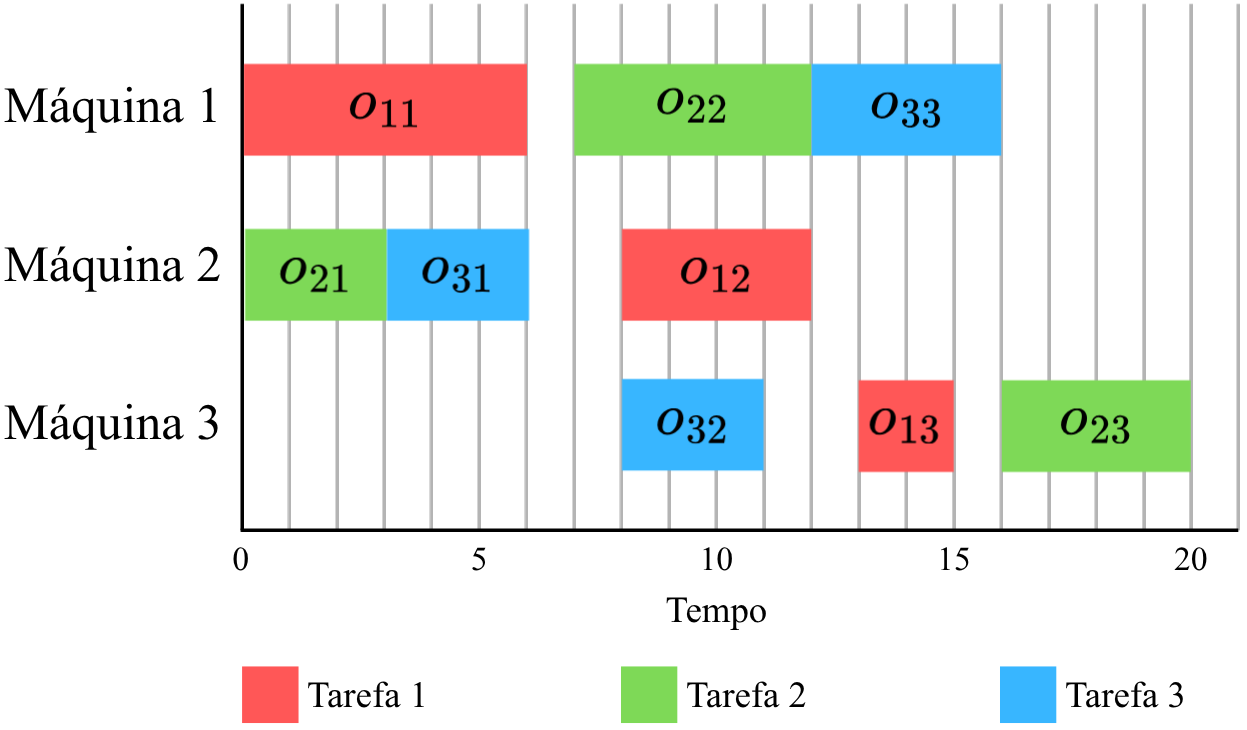
\includegraphics[width=0.75\linewidth]{img/exemplo_sol_jitjsp.png}
    \caption*{\small \textbf{Fonte:} Os Autores.}
\end{figure}

Dada a descrição e a modelagem do problema, podemos observar com mais detalhes o processo de encontrar uma solução para ele. Primeiramente, precisamos gerar uma sequência válida a partir da instância. Perceba que a instância do problema define uma ordem fixa para as operações de uma mesma tarefa, mas a ordem em que as operações utilizarão uma mesma máquina fica em aberto. Dessa forma, gerar uma sequência válida significa determinar a ordem de execução das operações em cada máquina. Para entender o processo de forma detalhada, precisamos introduzir o conceito de grafo disjuntivo na modelagem de problemas de agendamento.

\subsection{Grafo disjuntivo} \label{sect:grafo_disj}

Considere o grafo $G = (V, X, Y)$. Nesse grafo, para cada operação $o_{ik}$ de uma tarefa $J_i$, existe um vértice $u \in V$ representado por um par ordenado $(i,j)$, sendo $i$ o índice da tarefa e $j = M(o_{ik})$ o índice da máquina que processa essa operação. Além disso, o grafo possui dois conjuntos de arestas. As arestas conjuntivas $X$ e as arestas disjuntivas $Y$. As arestas conjuntivas são direcionadas e representam a ordem de processamento das operações de uma tarefa. Elas são dadas pela instância e existem apenas entre operações da mesma tarefa e, se a aresta $(u,v)$, $u,v \in V$, existe, a operação $u$ deve preceder a operação $v$. Enquanto isso, as arestas disjuntivas não são direcionadas e ligam operações que competem pela mesma máquina, isto é, se a aresta $\{u,v\}$, $u,v \in V$, existe, as operações $u$ e $v$ utilizam a mesma máquina. Adicionamos também dois vértices $s$ e $t$. O vértice $s$ possui $n$ arestas de saída na forma $(s,u)$ para cada vértice $u$ que representa a primeira operação de uma tarefa. Por outro lado, o vértice $t$ possui $n$ arestas de entrada na forma $(u,t)$ para cada vértice $u$ que representa a última operação de alguma tarefa. Definimos também uma função de pesos $w : V \to \mathbb{N}$ que mapeia cada vértice para um valor inteiro não negativo. Nesse âmbito, $w(s) = w(t) = 0$ \citep{pinedo2008}.

Considere novamente a instância do \ac{JITJSS} detalhada na Tabela \ref{tab:exemplo_agendamento}. A partir dessa instância, podemos gerar o grafo disjuntivo da Figura \ref{img:exemplo_grafo_disj}. Nessa figura, as arestas sólidas representam as arestas conjuntivas, enquanto as arestas tracejadas representam as arestas disjuntivas. De acordo com a definição do grafo disjuntivo para um problema de agendamento, podemos identificar as operações que utilizam uma mesma máquina. Na Figura em questão, os vértices em roxo representam as operações da máquina 1, os vértices em laranja representam a máquina 2 e os vértices em azul representam a máquina 3.

\begin{figure}[h!]
    \centering
    \caption{Grafo disjuntivo gerado a partir da instância de exemplo}
    \label{img:exemplo_grafo_disj}
    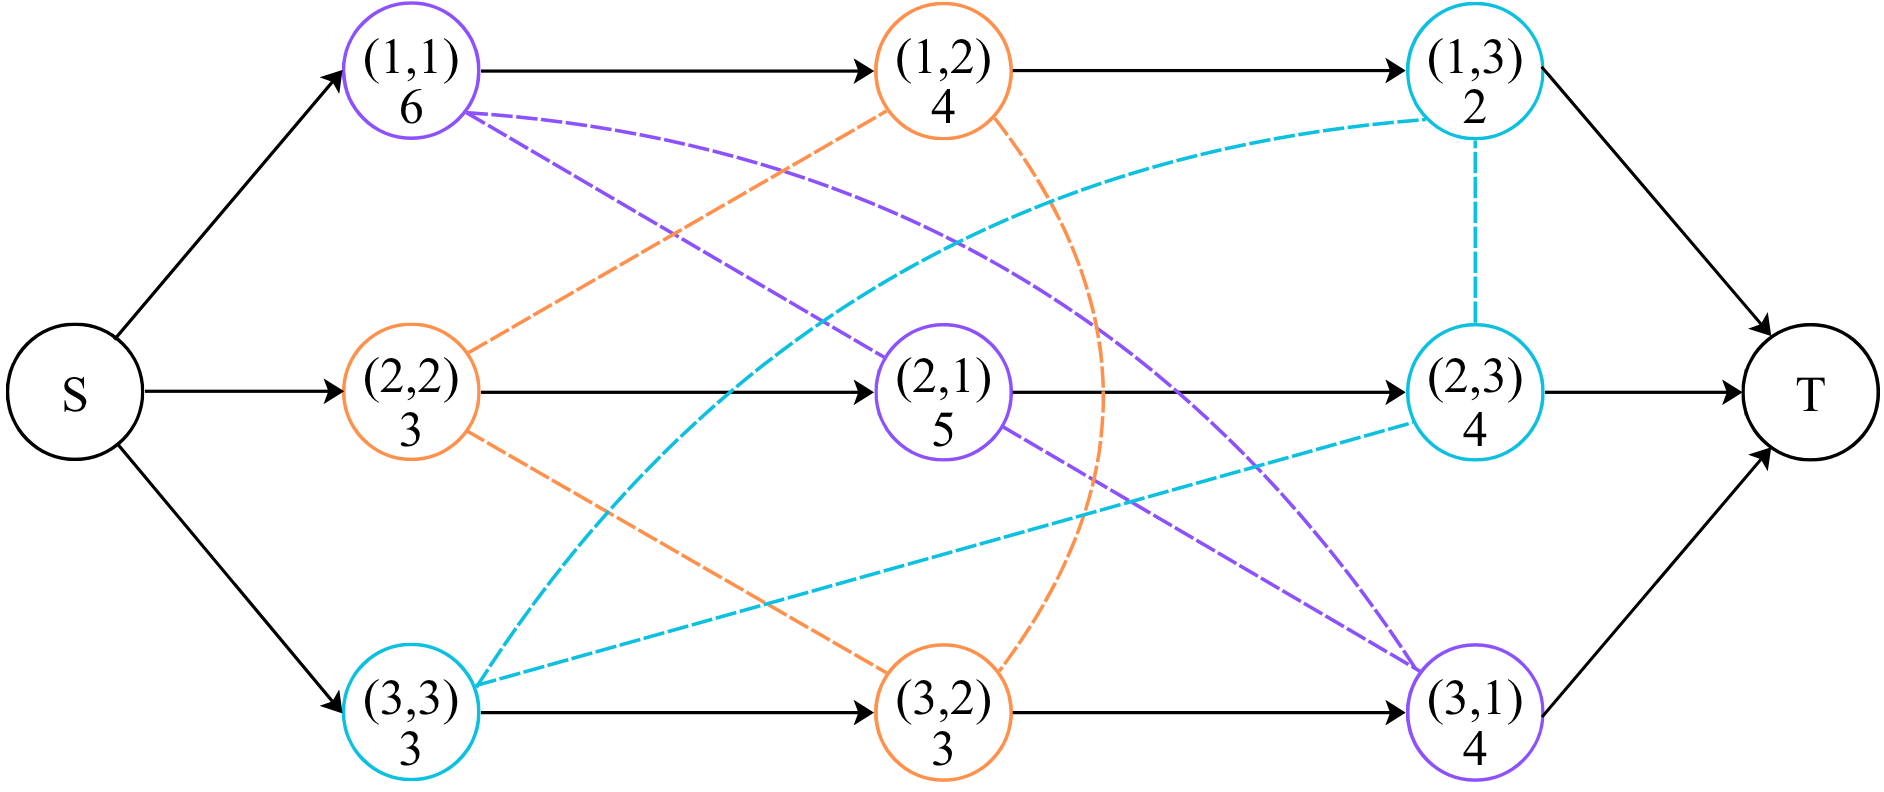
\includegraphics[width=0.75\linewidth]{img/grafo_disjuntivo.png}
    \caption*{\small \textbf{Fonte:} Os Autores.}
\end{figure}

Dessa forma, temos que, dada uma instância do problema, podemos gerar o grafo disjuntivo correspondente. Como mencionamos anteriormente, as arestas direcionadas do grafo disjuntivo implicam uma ordem de processamento das operações conectadas. Além disso, gerar uma sequência significa determinar a ordem de execução das operações em cada máquina. Por conseguinte, podemos definir que gerar uma sequência a partir de um grafo disjuntivo é o processo de selecionar direções para todas as arestas disjuntivas. Ao definir direções para todas as arestas disjuntivas, fazemos uma seleção completa e obtemos um grafo direcionado. Entretanto, para que a sequência seja viável, além da seleção completa, o grafo resultante precisa ser acíclico, pois um ciclo no grafo implicaria uma ordem de processamento impossível, na qual uma operação precederia a si mesma. Para a demonstração formal, veja \cite{pinedo2008}.


Podemos ver na Figura \ref{img:exemplo_dag} o mesmo grafo do exemplo anterior, mas com a seleção completa já aplicada. Dessa forma, observando o grafo, sabemos que a máquina 3 executará as operações $(3,3)$, $(1,3)$ e $(2,3)$ nessa ordem.

\begin{figure}[h!] 
    \centering
    \caption{Grafo direcionado acíclico que representa uma sequência viável}
    \label{img:exemplo_dag}
    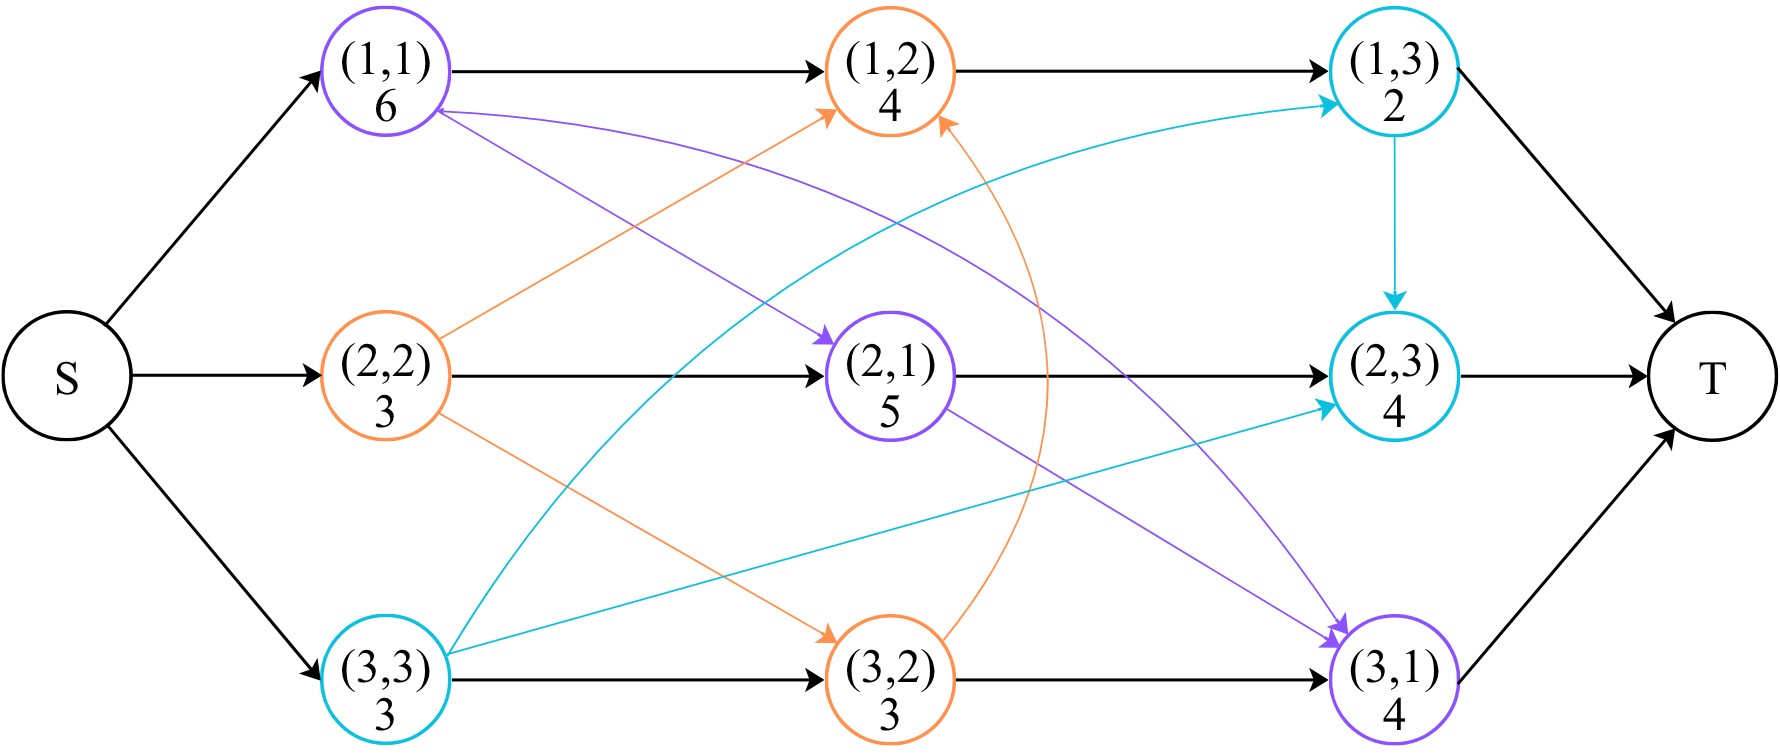
\includegraphics[width=0.75\linewidth]{img/grafo_selecao_completa.png}
    \caption*{\small \textbf{Fonte:} Os Autores.}
\end{figure}

Após encontrar uma sequência viável, precisamos avaliar a qualidade dessa sequência. Nesse sentido, uma das propriedades do grafo disjuntivo é que, após realizar a seleção das arestas disjuntivas, o caminho máximo do vértice $S$ ao $T$ é igual ao \textit{makespan} mínimo para essa seleção \citep{pinedo2008}. Por esse motivo, se nosso objetivo for minimizar o \textit{makespan}, dada uma sequência, podemos avaliar sua qualidade de forma ótima em tempo linear.

Por exemplo, o caminho máximo do grafo da Figura \ref{img:exemplo_dag} é composto pelos vértices $(1,1)$, $(1,2)$, $(1,3)$ e $(2,3)$, com peso total de 16. Podemos observar o agendamento que gera esse \textit{makespan} na Figura \ref{img:agendamento_makes}. O termo caminho crítico define esse percurso máximo, visto que as operações que o compõem impedem qualquer movimentação sem impacto no \textit{makespan}. Nesse sentido, nenhuma operação pertencente ao caminho crítico pode iniciar mais cedo sem que a sequência seja alterada.

Outra vantagem que temos ao minimizar o \textit{makespan}, sabendo o caminho crítico, é saber exatamente quais operações geram o \textit{makespan} de uma solução e, consequentemente, onde o agendamento exige modificações para alterar o \textit{makespan}. Essa informação auxilia o processo de minimização do \textit{makespan}, reduzindo o espaço de busca por melhorias.

\begin{figure}[h!] 
    \centering
    \caption{Agendamento ativo que minimiza o \textit{makespan}}
    \label{img:agendamento_makes}
    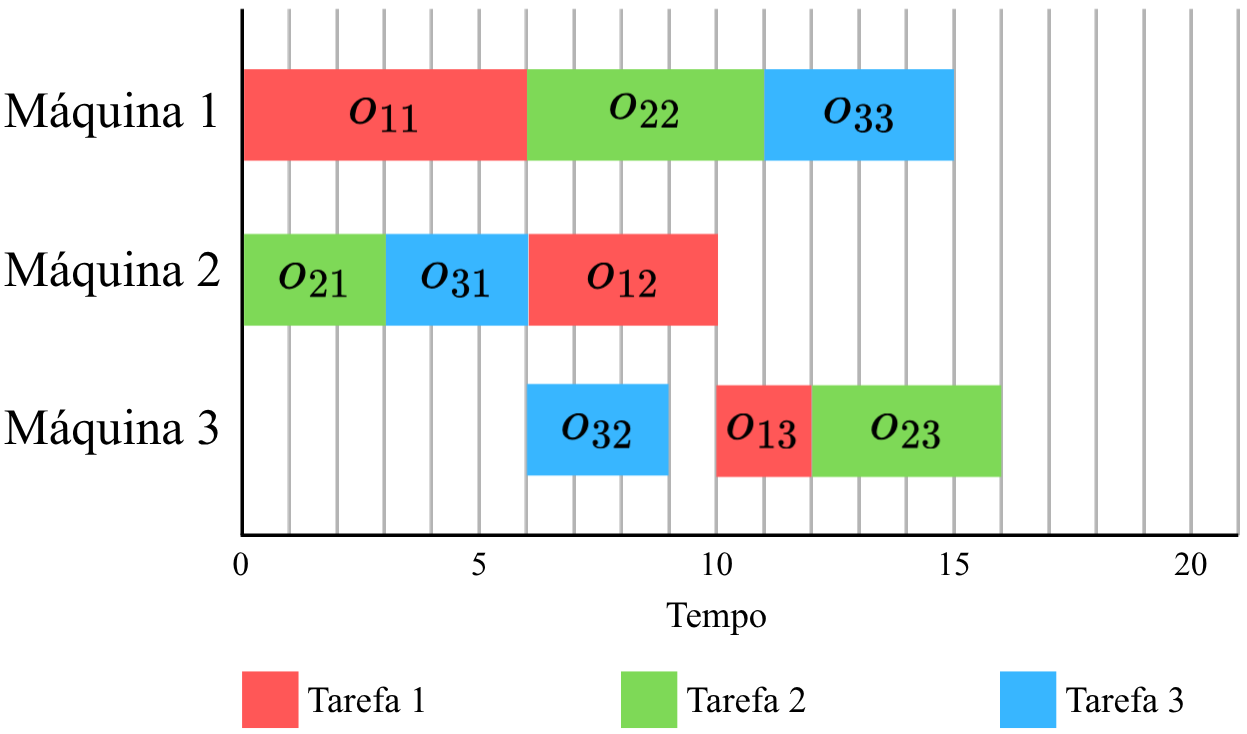
\includegraphics[width=0.75\linewidth]{img/agendamento_min_makes.png}
    \caption*{\small \textbf{Fonte:} Os Autores.}
\end{figure}

No entanto, se o nosso objetivo for minimizar as penalidades de adiantamento e atraso, não temos uma forma tão simples e rápida de gerar um agendamento ótimo a partir de uma sequência. O agendamento representado na Figura \ref{img:agendamento_makes} demonstra que agendar as operações o mais cedo possível não significa minimizar as penalidades, pois esse processo tende a gerar penalidades de adiantamento. Esse agendamento, por exemplo, gera uma penalidade total de 8,4, das quais 7,7 correspondem a penalidades por adiantamento. Ademais, poderíamos atrasar o início de algumas operações para que as penalidades fossem menores, o que nos levaria ao agendamento da Figura \ref{img:exemplo_sol_jitjsp}, que é ótimo para essa sequência específica. Veja a seção \ref{sect:bibjitjsp} para uma revisão bibliográfica que inclui as formas de gerar agendamentos utilizadas na literatura do \ac{JITJSS}.

\subsection{Algoritmos para geração de agendamentos} \label{sect:algs_constrs}

Nesta seção, apresentamos formas de gerar uma sequência viável por meio de exemplos de algoritmos. Nesse sentido, a literatura classifica procedimentos que constroem um agendamento do zero como construtivos. Estes algoritmos, de forma geral, precisam selecionar operação por operação a ser agendada até que todas sejam agendadas. Chamamos de regras de despacho as diferentes formas de selecionar qual operação agendar entre um conjunto de operações \citep{pinedo2008}. Tais algoritmos construtivos são capazes de utilizar qualquer regra de despacho internamente. Dessa forma, podemos definir um algoritmo que gera um agendamento baseado apenas em uma regra de despacho arbitrária.

Sejam, respectivamente, $J$, $M$ e $O$ os conjuntos de tarefas, máquinas e operações de um problema de agendamento. Dados esses conjuntos, definimos $o_{ik}$ como sendo a $k$-ésima operação da tarefa $i$. O algoritmo mantém uma lista $L$ de todas as operações para as quais todas as suas antecessoras já foram agendadas, isto é, se $o_{ik} \in L$, então as operações $o_{ix}$, nas quais $x < k$, já foram agendadas. O procedimento inicializa a lista $L$ com a primeira operação de cada tarefa e, a cada iteração, o algoritmo seleciona uma operação $o_{ik} \in L$ para ser agendada de acordo com uma regra de despacho e adiciona em $L$ a operação $o_{ik+1}$. Ao final de $|O|$ iterações, o algoritmo conclui o agendamento de todas as operações em $O$ \citep{pinedo2008}.

Outro algoritmo um pouco mais sofisticado é o \ac{GT} \citep{giffler1960algorithms} para geração de agendamentos ativos. Um agendamento é ativo quando não é possível alterar a posição de uma operação no agendamento para que ela inicie mais cedo sem que um atraso em outra operação seja causado, em outras palavras, o agendamento não possui tempo ocioso entre duas operações no qual fosse possível agendar outra operação. Por exemplo, o agendamento da Figura \ref{img:agendamento_makes} é um agendamento ativo. O algoritmo \ac{GT} utiliza as mesmas estruturas que o algoritmo descrito anteriormente, mas, antes de utilizar uma regra de despacho para selecionar uma operação, ele realiza filtros na lista $L$ para que apenas operações que mantém o agendamento ativo sejam escolhidas.

Seja $P(o_{ik}) \in \mathbb{N}$ o tempo de processamento da operação $o_{ik}$ e $A(o_{ik}) \in O$ a operação que antecede $o_{ik}$ na mesma máquina. Definimos o tempo de término de uma operação $C(o_{ik}) = max(C(o_{ik-1}), C(A(o_{ik})) + P(o_{ik})$. O algoritmo \ac{GT} seleciona em $L$ a operação $o'$ com menor tempo de término $C'$. A partir dessa operação, o algoritmo cria a lista $L_1 \subseteq L$ que contém as operações $o''$ as quais $M(o'') = M(o')$ e $C(o'') \le C'$. O algoritmo, então, aplica uma regra de despacho na lista $L_1$ para selecionar a operação $o_{ik}$ que será agendada, remove $o_{ik}$ de $L$ e adiciona $o_{ik+1}$ em $L$ se $o_{ik+1} \in O$. Após $|O|$ iterações, o algoritmo produz um agendamento viável e ativo.

\section{Configuração Automática de Algoritmos}

No processo de desenvolver estratégias de resolução para problemas inerentemente difíceis como o \ac{JITJSS}, uma das alternativas que possuímos é utilizar heurísticas. Uma heurística resolve o problema em tempo viável, mas não garante a qualidade das soluções que encontra, no sentido de que não é possível demonstrarmos que as soluções são ótimas ou que possuem algum limite de aproximação da solução ótima \citep{talbi}.

Durante o desenvolvimento dessas estratégias, os pesquisadores perceberam que grupos de diferentes heurísticas para problemas diferentes possuem diversas características em comum. Por exemplo, toda heurística de busca possui algum tipo de construção, recombinação ou modificação de soluções dentro do seu processo de exploração do espaço de busca. Esses conceitos são independentes de características específicas de cada problema. Por outro lado, ao observarmos a aplicação desses conceitos na literatura, percebemos estratégias específicas que os autores implementam para servir às peculiaridades do problema-alvo \citep{zbb}.

A partir dessas ideias, abstraímos os conceitos comuns entre diferentes estratégias e definimos métodos que podemos aplicar em qualquer problema, mas que possuem lacunas que devemos preencher com os componentes específicos ao problema que estamos resolvendo. A comunidade científica chama esses métodos genéricos de meta-heurísticas \citep{zbb}.

O desenvolvimento de meta-heurísticas eficientes em resolver um problema leva tempo e exige do projetista um conhecimento profundo das características do problema. As meta-heurísticas tendem a facilitar esse processo por meio da generalização de métodos em comum que funcionaram para diferentes problemas. Ainda assim, desenvolver uma meta-heurística eficiente é um processo custoso. Nessa perspectiva, os projetistas de meta-heurísticas precisam tomar diversas decisões de projeto, tanto de alto quanto de baixo nível. Esses projetistas podem basear essas decisões em testes exaustivos, buscando encontrar uma configuração que retorne os melhores resultados. Porém, essa abordagem é tediosa, propensa a erros e dificilmente reproduzível \citep{birattari2009tuning}.

Com o avanço e maior disponibilidade do poder computacional e visando mitigar o problema de configurar heurísticas, a comunidade científica propôs diversos métodos de \ac{AAC}. Dessa forma, os pesquisadores podem executar o trabalho repetitivo e tedioso automaticamente, ganhando tempo para, por exemplo, desenvolver novas estratégias para a resolução de problemas \citep{birattari2009tuning}.

Esta seção aborda a \ac{AAC} como um problema de otimização e as principais ferramentas para resolvê-lo, detalhando inicialmente os conceitos fundamentais de vizinhanças e meta-heurísticas. No entanto, considerando o objetivo do presente trabalho, não realizaremos uma revisão abrangente de todos os tipos de meta-heurísticas, mas detalharemos apenas aquelas relacionadas ao domínio do projeto. Dessa forma, para detalhes e definições sobre meta-heurísticas, nos referimos aos trabalhos de \cite{talbi} e \cite{zbb}.

% Esta seção aborda conceitos de configuração automática. Primeiro, ela define conceitos fundamentais de meta-heurísticas e explica as meta-heurísticas mais importantes para o presente trabalho. Em seguida, explica a configuração automática enquanto um problema de otimização e apresenta as principais ferramentas utilizadas no processo de configuração automática. Muitas estratégias heurísticas citadas ao longo do trabalho não serão completamente detalhadas. Dessa forma, para detalhes e definições de cada meta-heurística citada no restante deste trabalho, veja .

\subsection{Vizinhanças}

Dado o conjunto de todas as soluções $S$ de um problema, \cite{talbi} define uma vizinhança como um mapeamento de cada solução $s \in S$ para um subconjunto de soluções $N(s) \subseteq S$. Chamamos de vizinha de $s$ uma solução $s' \in N(s)$. O mapeamento da vizinhança modifica soluções sistematicamente para gerar novas soluções. Por isso, a vizinhança é uma componente específica do problema-alvo, isto é, sua forma e eficiência dependem exclusivamente das características do problema. Isso é verdade, pois modificar uma solução inclui manipular a representação da solução, que varia entre problemas e até mesmo entre diferentes abordagens sobre o mesmo problema \citep{talbi}.

O projetista de uma vizinhança deve considerar algumas características durante o desenvolvimento. Uma delas é a localidade da vizinhança; essa propriedade consiste no impacto que alterações na representação de uma solução têm sobre a qualidade da solução. Se pequenas alterações na representação causam pequenas mudanças na solução, a vizinhança possui alta localidade. Por outro lado, se pequenas alterações na representação causam grandes mudanças na solução, a vizinhança possui baixa localidade. Diante disso, uma exploração do espaço de busca por meio de uma vizinhança com alta localidade é mais refinada e sistemática \citep{talbi}.

Outro ponto importante é o tamanho da vizinhança. Gerar e explorar uma vizinhança muito grande pode ter um custo alto e, consequentemente, atrapalhar o processo de busca. Por outro lado, vizinhanças muito restritas e, consequentemente, pequenas, podem ignorar soluções promissoras no espaço de soluções. \citep{talbi}.

Com o conceito de vizinhança estabelecido, podemos introduzir o conceito de ótimo local. Esse conceito é importante pois diversas meta-heurísticas mais sofisticadas implementam múltiplas técnicas para evitar ótimos locais. \cite{talbi} define um ótimo local como uma solução $s'$ tal que, para toda solução vizinha $s'' \in N(s')$, temos que $f(s') \leq f(s'')$. Um ótimo global, por sua vez, é uma solução $s'$ que, para qualquer solução $s''$ do espaço de busca, $f(s') \leq f(s'')$ \citep{talbi}. Note que, por definição, todo ótimo global é também um ótimo local, mas o inverso não é verdadeiro. A Figura \ref{img:exemplo_minimos_locais} apresenta um gráfico que representa os valores de $f$ pelo espaço de busca e indica os ótimos locais e um ótimo global.

\begin{figure}[h!] 
    \centering
    \caption{Mínimos locais em relação à função objetivo no espaço de soluções}
    \label{img:exemplo_minimos_locais}
    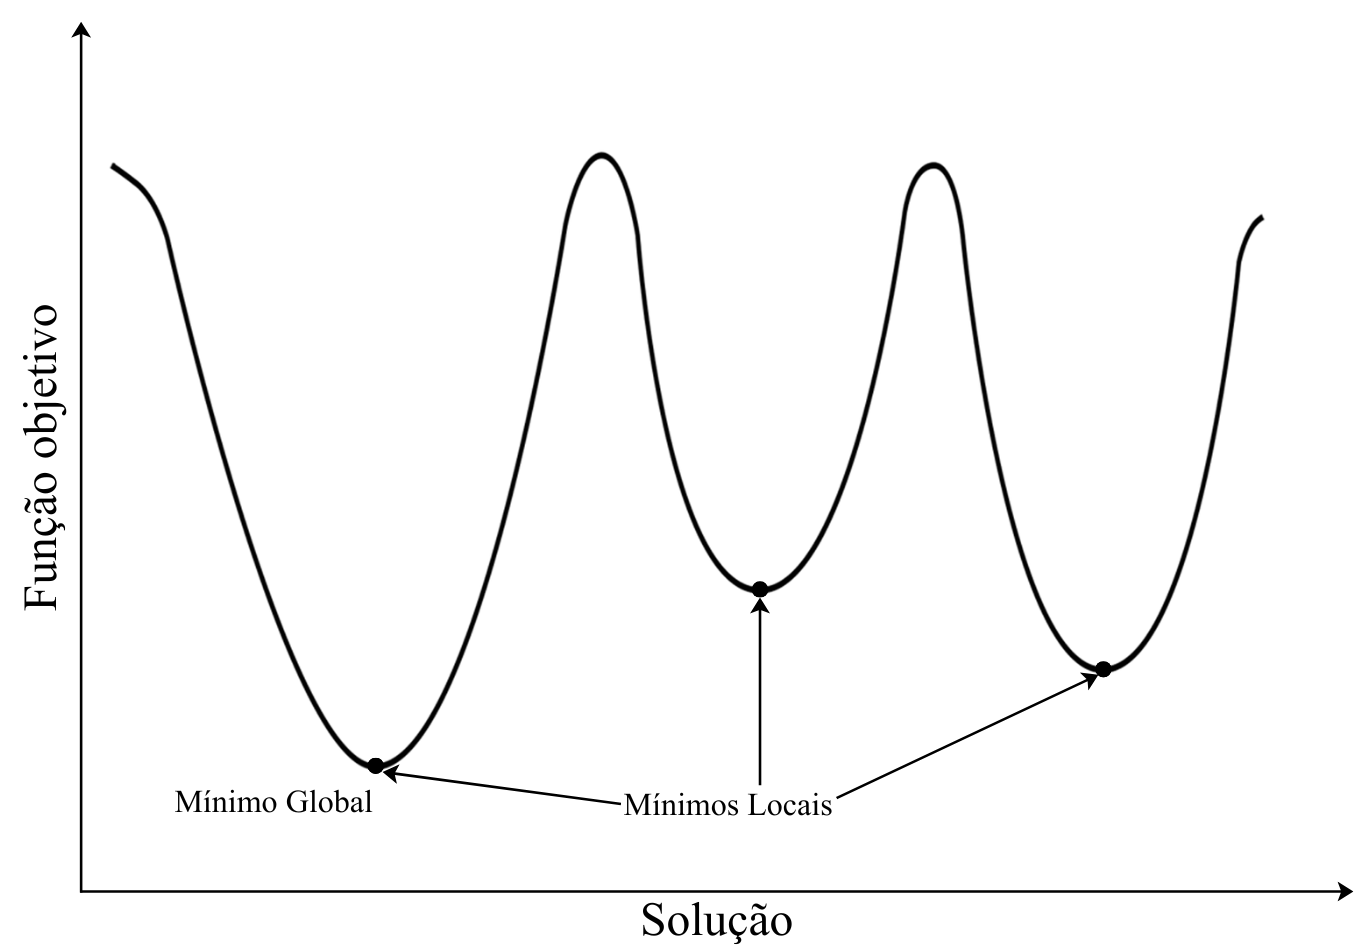
\includegraphics[width=0.75\linewidth]{img/minimos_locais.png}
    \caption*{\small \textbf{Fonte:} Adaptado de \cite{talbi}}
\end{figure}

\subsection{Meta-heurísticas} \label{sect:meta}

Como mencionamos anteriormente, as meta-heurísticas são estratégias de alto nível que podemos aplicar a qualquer problema. Em vista disso, a Busca Local (do inglês, Local
Search -- \acs{LS}) é uma das meta-heurísticas mais básicas e, por isso, as meta-heurísticas mais sofisticadas utilizam seus conceitos internamente. Dada uma solução inicial $s_0$, a cada iteração $i$, a busca local gera a vizinhança $N(s_i)$ da solução $s_i$. Assim, a busca local seleciona uma solução $s_{i+1} \in N(s_i)$ tal que $f(s_{i+1}) < f(s_i)$, em outras palavras, seleciona uma solução que melhora a função objetivo. Por fim, o algoritmo finaliza o processo de busca quando não existe nenhuma solução $s' \in N(s_i)$ de forma que $f(s') < f(s_i)$. Por esse motivo, a busca local não consegue escapar de ótimos locais no espaço de busca \citep{talbi}.

Podemos realizar a exploração do espaço de busca e a seleção de vizinhos na busca local de diferentes formas. Uma delas, a seleção por melhor melhora, consiste em selecionar o melhor vizinho de uma solução a cada iteração, isto é, tendo uma solução $s_i$, o algoritmo seleciona a vizinha de $s_i$ que oferece o máximo de melhoria na função objetivo em relação a $f(s_i)$. Utilizar esse tipo de seleção significa gerar e avaliar todos os vizinhos da solução a cada iteração. Esse processo pode ter um custo elevado em vizinhanças grandes \citep{talbi}.

Outra forma de selecionar vizinhos consiste em selecionar o primeiro vizinho de $s_i$ que melhora a função objetivo. Por isso, ao contrário da primeira opção, o algoritmo não precisa gerar nem avaliar toda a vizinhança. Isso gera uma exploração do espaço de busca mais rápida; porém, corremos o risco de que o processo ignore boas soluções simplesmente pela ordem de geração e avaliação dos vizinhos. Chamamos essa segunda estratégia de seleção por primeira melhora \citep{talbi}.

O maior problema de uma busca local simples é a incapacidade de escapar de ótimos locais. Por esse motivo, buscas locais tendem a finalizar o processo de busca precocemente e sem realizar uma exploração satisfatória no espaço de busca. Com isso em mente, apresentamos o conceito de perturbação de uma solução. Meta-heurísticas mais complexas utilizam esse processo com o objetivo de escapar de ótimos locais. Ele geralmente se aplica aos ótimos locais e consiste em realizar alguma modificação da solução que seja significativa o suficiente para que a solução modificada se afaste do ótimo local \citep{talbi}. Por exemplo, no gráfico da Figura \ref{img:exemplo_perturbacao}, temos duas funções de perturbação, $g'$ e $g''$. Nesse caso da imagem, a função $g'$ não fez uma perturbação efetiva, pois a solução gerada não é diferente o suficiente para gerar um mínimo local diferente. Por outro lado, a função $g''$ gera uma solução que levará o processo de busca a um mínimo local diferente e melhor.

\begin{figure}[h!] 
    \centering
    \caption{Transformações de mínimos locais por funções de perturbação.}
    \label{img:exemplo_perturbacao}
    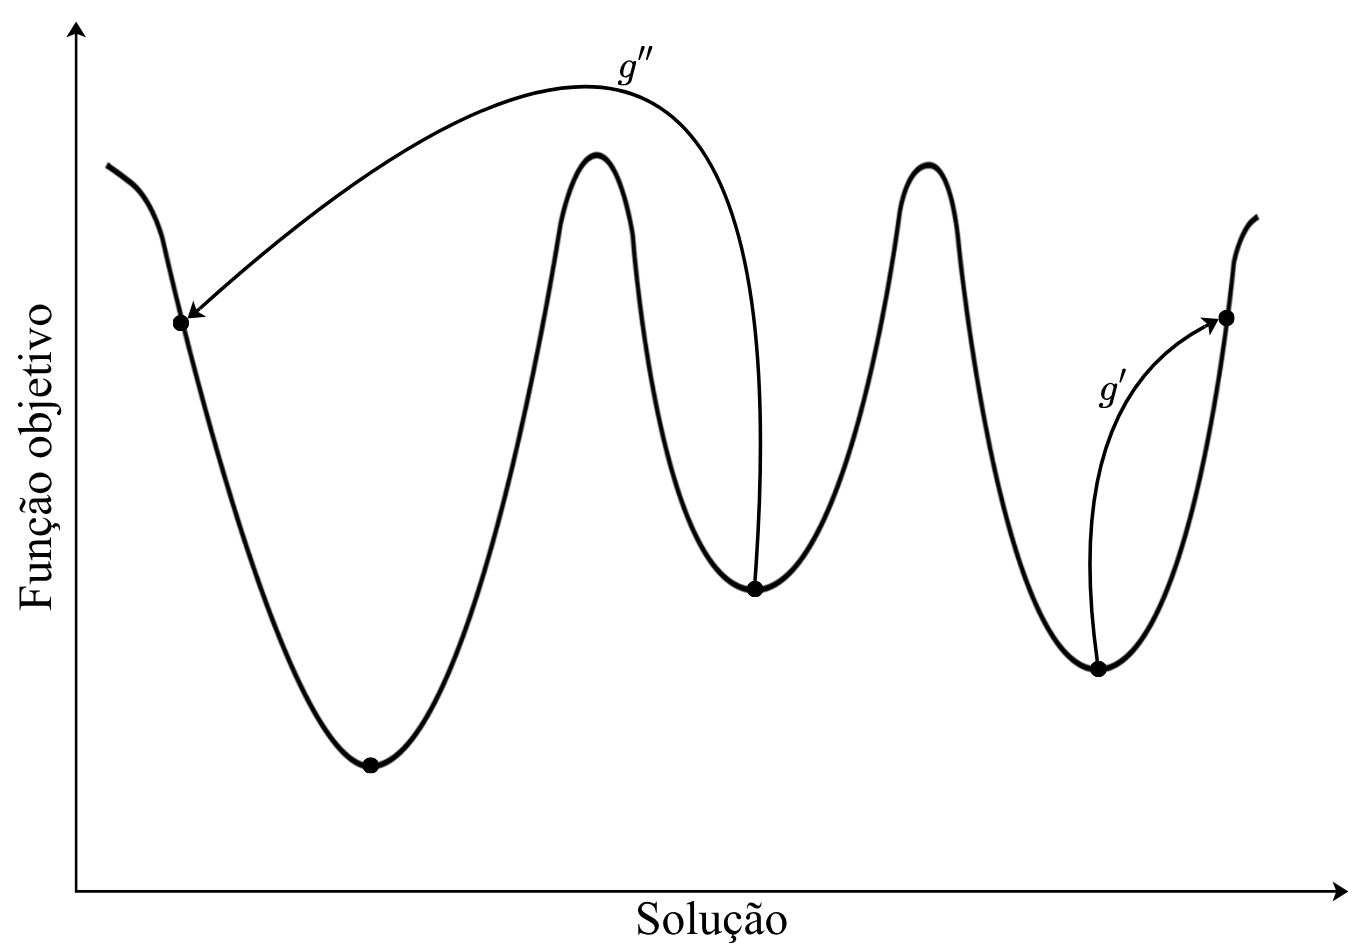
\includegraphics[width=0.75\linewidth]{img/exemplo_perturbacao.png}
    \caption*{\small \textbf{Fonte:} Os Autores.}
\end{figure}

A Busca Local Iterada (do inglês, Iterated Local
Search -- \acs{ILS}) é um exemplo de meta-heurística que utiliza um processo de perturbação em seu processo de busca. Ela realiza, iterativamente, buscas locais com diferentes soluções iniciais para encontrar diferentes ótimos locais. Em cada iteração, ela utiliza uma perturbação do ótimo local encontrado na iteração anterior \citep{talbi}. Algumas características da \ac{ILS} incluem a possibilidade de utilizar qualquer heurística de solução única como método de busca, isto é, o processo de encontrar um ótimo local a cada iteração é uma caixa-preta. Nesse sentido, essa caixa-preta deve receber uma solução e encontrar um ótimo local \citep{talbi}.

Algumas meta-heurísticas renomeiam o processo de perturbação. Por exemplo, a Busca em Vizinhança Variável (do inglês, Variable Neighborhood Search -- \acs{VNS}) chama esse processo de \textit{shake}. Essa meta-heurística se apoia na ideia de que diferentes vizinhanças de um mesmo problema exploram subespaços de busca diferentes. Mais especificamente, podemos dividir o processo de busca na \ac{VNS} em três fases: \textit{Shake}, busca local e \textit{move}. Dada uma lista de estruturas de vizinhança $N = \{N_1, N_2,...N_{n-1}, N_n\}$, a cada iteração, a \ac{VNS} realiza o \textit{shake} de uma solução inicial $s$ pela vizinhança atual $N_k \in N$, isto é, o algoritmo seleciona uma solução $s'$ aleatoriamente da vizinhança $N_k(s)$. Após o \textit{shake}, a \ac{VNS} aplica um processo de busca local sobre a solução $s'$, encontrando um ótimo local $s''$. Por fim, caso $f(s'') < f(s)$, a \ac{VNS} realiza o \textit{move}, ou seja, seleciona $s''$ como a nova solução base e redefine $k=1$; caso contrário, mantém a solução e incrementa $k$, $k = k+1$ \citep{talbi}.

% Por fim, apesar de não garantirem a qualidade das soluções obtidas, as meta-heurísticas se provaram excelentes opções para resolver problemas. Por exemplo, o estado da arte para o \ac{JITJSS} é composto majoritariamente por meta-heurísticas como os algoritmos \ac{VNS} de \cite{ahmadian2021meta} e \cite{wang2014variable}, a busca adaptativa em grandes vizinhanças de \cite{abderrazzak2022adaptive} e o algoritmo evolucionário de \cite{dos2010combination}.

Dando continuidade às estratégias de evasão de mínimos locais, também podemos utilizar a Busca Tabu (do inglês, \textit{Tabu Search} -- \acs{TS}). Essa meta-heurística é semelhante à busca local no sentido de que inicia a busca a partir de uma solução inicial $s_0$ e explora o espaço de busca iterativamente, selecionando novas soluções que melhoram a função objetivo. Porém, a busca tabu não encerra a busca ao chegar a um ótimo local no espaço de busca. Ao invés disso, a busca seleciona uma solução que piora a função objetivo para escapar do ótimo local. Nesse sentido, ela seleciona o vizinho com o menor valor da função objetivo, mesmo que ele não seja melhor que a solução que o gerou \citep{talbi}.

% Durante a exploração do espaço de soluções na busca local, a solução da iteração atual é sempre melhor que todas as soluções de iterações anteriores. Por outro lado,
Ao selecionar soluções que pioram a função objetivo, a busca tabu permite que soluções selecionadas em iterações anteriores sejam melhores que a solução da iteração atual. Por isso, é intuitivo pensar que a busca pode ficar presa em um ciclo infinito de pioras e melhoras da função objetivo. Porém, a busca tabu utiliza uma memória para evitar selecionar soluções repetidas. Ela implementa essa memória em uma lista tabu de movimentos realizados, e não seleciona novas soluções que desfazem esses movimentos tabu. É importante mencionar que a lista tabu mantém os estados da busca por um período denominado $tenure$ \citep{talbi}.

% A implementação da lista tabu depende de características específicas do problema-alvo. Armazenar as soluções integralmente nem sempre é viável pelo espaço de armazenamento necessário e pelo custo de verificar se uma solução está na lista. Por isso, em certos problemas, é mais vantajoso armazenar uma informação parcial das soluções e, com isso, ganhar eficiência de verificação da lista em detrimento da precisão de verificação \citep{talbi}.
% Por exemplo, podemos implementar a lista tabu de forma que ela armazene os movimentos que o algoritmo realizou na solução entre cada iteração e barrar novas soluções que revertam esses movimentos. Essa estratégia torna eficiente verificar se a lista tabu permite um movimento, mas não impede que o algoritmo selecione soluções repetidas, visto que, em certos problemas, é possível retornar à mesma solução por diferentes sequências de modificações \citep{talbi}.  

A implementação ideal de uma meta-heurística sobre um problema deveria obter bons resultados em todos os tipos diferentes de instâncias do problema. Porém, construir soluções que atinjam essa generalização de forma completa nem sempre é possível \citep{birattari2009tuning}. Por exemplo, suponha um algoritmo de busca local para um certo problema $X$, talvez a seleção por primeira melhora seja a melhor opção para um determinado grupo de instâncias, mas, para um grupo diferente de instâncias, a seleção por melhor melhora seja ideal. O projetista precisa escolher qual tipo de seleção implementar, ou por primeira melhora, ou por melhor melhora, ou até mesmo por uma terceira forma híbrida. Esse tipo de decisão se repete constantemente no desenvolvimento de soluções. Nesses casos, o projetista pode definir e implementar uma das opções ou implementar todas e permitir ao usuário do algoritmo escolher a abordagem por meio de um parâmetro. Dessa forma, o usuário pode decidir as estratégias mais adequadas aos tipos de instâncias em questão \citep{birattari2009tuning}.

Definir parâmetros customizáveis parece resolver o problema, pois gera algoritmos mais flexíveis. Porém, mesmo assim, o projetista ainda precisou realizar uma série de decisões que compõem a base desse algoritmo flexível. Além disso, o usuário também precisará definir uma série de parâmetros de acordo com suas necessidades. Diante disso, uma das alternativas para tomar tais decisões é realizar múltiplos testes até encontrar uma configuração razoável. Porém, essa abordagem tem alguns problemas \citep{birattari2009tuning}.

Primeiramente, para que esse processo seja efetivo, o indivíduo que configurar o algoritmo precisa ter um conhecimento profundo do problema em questão, além de conhecer detalhadamente o algoritmo em si. Além disso, esse tipo de configuração pode invalidar completamente os resultados da comparação entre algoritmos. Por exemplo, considere que um projetista comparou dois algoritmos $A$ e $B$. Nesse processo, ele passou 75\% do seu tempo configurando o algoritmo $A$ e os outros 25\% configurando o $B$. Independentemente de qual algoritmo obteve os melhores resultados, o viés da configuração invalida a comparação. Ou seja, os resultados dependem da imparcialidade do projetista que configurou os algoritmos \citep{birattari2009tuning}.

É nesse contexto que surge a necessidade de métodos científicos e formais para configurar algoritmos. 

% Pois, dado que um ótimo local possui características de uma boa solução, pode ser mais vantajoso continuar a busca a partir dos seus vizinhos ao invés de voltar para uma solução aleatória \citep{talbi}.
% Essa estratégia é baseada na ideia de que, sendo o ótimo local a melhor solução em uma certa área do espaço de busca, ele possui características de uma boa solução e, por isso, devemos manter algumas delas para alcançar outra boa solução \citep{talbi}.

% Além disso, o processo de perturbação do ótimo local é outro componente importante para a \ac{ILS}. Esse procedimento tem como objetivo afastar o processo de busca dos ótimos locais encontrados em cada iteração. O impacto da perturbação na solução pode variar a depender da estratégia. Por exemplo, quando o processo de busca utilizado é altamente eficiente, realizar uma pequena modificação na solução fará com que o processo de busca encontre o mesmo ótimo local na próxima iteração, fazendo a \ac{ILS} ficar presa em um ciclo \citep{talbi}.

% Por fim, após realizar a perturbação e o processo de busca sobre o ótimo local perturbado, a \ac{ILS} utiliza, na próxima iteração, o novo ótimo local encontrado pela heurística de busca apenas se ele passar em um critério pré-determinado. Esse critério varia em um espectro no qual um dos extremos é aceitar apenas soluções que melhoram a função objetivo e o outro extremo é aceitar soluções independentemente de seus valores na função objetivo. Ao utilizarmos uma \ac{ILS} para resolver um problema, é importante encontrarmos um ponto nesse espectro que seja adequado às particularidades do problema-alvo \citep{talbi}. 

\subsection{Problema de Configuração \textit{offline} de algoritmos}

Dado o contexto de utilização da \ac{AAC}, podemos definir a configuração de algoritmos como um problema de otimização. Perceba que o objetivo da configuração de algoritmos é, dado um algoritmo e instâncias de um problema, determinar os parâmetros do algoritmo que maximizam sua performance nessas instâncias \citep{birattari2009tuning}. Nesta subseção, formalizaremos esse problema.

Chamamos o problema de \textit{offline} pela forma como ele realiza a otimização da configuração. Em métodos \textit{offline}, a busca no espaço de configurações ocorre em uma fase de treinamento e a melhor configuração encontrada é, então, utilizada em produção. Usualmente, utilizamos um conjunto de instâncias de treinamento e, como forma de validar as configurações obtidas, utilizamos um conjunto diferente de instâncias para testar essas configurações obtidas \citep{birattari2009tuning}.

Definimos aqui o problema de configuração de algoritmos. Seja $\mathcal{A}$ um algoritmo com $n$ parâmetros $p_i$ e $1 \leq i \leq n$, de forma que cada parâmetro $p_i$ possua domínio $\Theta_i$. Temos que o espaço de configurações $\Theta \subseteq \Theta_1 \times \Theta_2 \times \ldots \times \Theta_n$ contém todas as combinações de parâmetros válidas do algoritmo $\mathcal{A}$. Dessa maneira, dado um conjunto de instâncias $\Pi$ e uma função de custo $c(\theta, \pi)$ que mede o custo de executar $\mathcal{A}$ sobre a instância $\pi \in \Pi$ com uma configuração $\theta \in \Theta$, o objetivo do problema é encontrar uma configuração $\theta^* \in \Theta$ que minimize o custo de $\mathcal{A}$ sobre todo o conjunto $\Pi$. Podemos ver essa função objetivo na Equação \ref{eq:2.9}, onde $\mathcal{C}$ é uma função agregada de $c(\theta, \pi)$ sobre todas as instâncias $\pi \in \Pi$ \citep{souza2022automatic}.

\begin{align} \label{eq:2.9}
&\theta^* \in \operatorname{argmin}\mathcal{C}(\theta, \Pi) &&\theta \in \Theta
\end{align}

Podemos utilizar como função agregada $\mathcal{C}$, a exemplo, o desempenho médio em todas as instâncias $\mathcal{C}(\theta, \Pi) = \sum_{\pi \in \Pi} c(\theta, \pi) / |\Pi|$ ou o pior desempenho encontrado em qualquer uma das instâncias $\mathcal{C}(\theta, \Pi) = \max_{\pi \in \Pi} c(\theta, \pi)$.

Um algoritmo parametrizado pode ter parâmetros de diferentes tipos. Nesse sentido, parâmetros categóricos definem um conjunto fixo de opções para o algoritmo. Utilizamos esse tipo de parâmetro frequentemente para definir estratégias do algoritmo para atingir um mesmo fim, por exemplo, qual vizinhança utilizar em uma busca local. Os parâmetros também podem ser ordinais, isto é, seus valores possuem uma relação de ordem intrínseca. Por exemplo, considere o mesmo parâmetro de escolha de vizinhança em uma busca local, mas, agora, as vizinhanças estão ordenadas pelo seu tamanho. Por fim, também temos os parâmetros numéricos. Eles mapeiam valores inteiros ou reais do algoritmo, como, por exemplo, constantes utilizadas em cálculos e funções, ou a temperatura inicial de um algoritmo de Recozimento Simulado (do inglês, \textit{Simulated Annealing} - \acs{SA}) \citep{lopez2016irace}.

Além dos diferentes tipos, podemos definir relações entre parâmetros. Uma relação condicional acontece quando um parâmetro pode ser definido apenas se outro parâmetro também for definido. Por exemplo, em um algoritmo que utiliza diferentes meta-heurísticas definidas por um parâmetro, só faz sentido definir o parâmetro \textit{tenure} se o algoritmo alvo utilizar a meta-heurística Busca Tabu. Parâmetros também podem impor restrições a outros parâmetros. Por exemplo, em um algoritmo evolutivo, o número de indivíduos selecionados para o processo de \textit{crossover} não pode ser maior do que o tamanho da população. Por fim, algumas combinações de parâmetros não são permitidas, pois podem causar erros ou comportamentos indefinidos no algoritmo \citep{lopez2016irace}.

Assim, podemos definir uma instância do problema de configuração de algoritmos. Ela é uma sêxtupla $I=(\mathcal{A}, \Theta, \Pi, c , B, S)$ onde $\mathcal{A}$ é o algoritmo alvo da configuração, $\Theta$ é o espaço de configurações, $\Pi$ é um conjunto de instâncias de treinamento, $c$ é uma métrica de custo, $B$ é a quantidade de recursos disponíveis para configuração e $S$ é um conjunto de informações adicionais \citep{hutter2009paramils}. Mais especificamente, o recurso $B$ diz respeito ao recurso computacional disponível para realizar essa configuração e, usualmente, medimos em iterações ou em tempo de processamento. Além disso, também temos as configurações adicionais $S$ que incluem, por exemplo, fatores relacionados ao processo de configuração, a alguma configuração do algoritmo ou às instâncias de teste. Por exemplo, o conjunto $S$ pode conter configurações iniciais para o configurador, o critério de parada do algoritmo ou argumentos específicos para certas instâncias.

Mesmo com o problema formalizado, precisamos de maneiras de resolvê-lo. Uma abordagem possível seria fazer isso manualmente através de testes e observação das melhores configurações. Porém, como já mencionamos, esse tipo de processo ocupa muito tempo dos projetistas de algoritmos, principalmente para testar configurações ruins. Além disso, o processo é muito difícil de replicar e pode gerar configurações enviesadas que, consequentemente, produzem resultados inválidos. Por esses motivos, precisamos de métodos sistemáticos para resolver o problema da configuração de algoritmos \citep{birattari2009tuning}

\subsection{Processo de configuração automática e configuradores} \label{sect:ref_conf_auto_configuradores}

O processo de \ac{AAC} consiste em utilizar os recursos computacionais disponíveis para explorar o espaço de configurações. Chamamos a ferramenta que realiza essa exploração de configurador. Na Figura \ref{img:diagrama_configurador} podemos observar a organização e o fluxo dos componentes de um configurador. O algoritmo configurador recebe como entrada a instância definida na subseção anterior. A partir disso, ele realiza chamadas do algoritmo $\mathcal{A}$ sobre uma determinada instância $\pi$ com a configuração $\theta$. O algoritmo $\mathcal{A}$, então, retorna o valor da métrica $c$ para a instância e configuração fornecidas. Dessa maneira, o configurador avalia configurações e explora o espaço de busca sistematicamente. Ao consumir todo o recurso computacional $B$, o configurador retorna a configuração (ou configurações) que teve o melhor desempenho agregado nas instâncias de treinamento. \citep{hutter2009paramils}.

\begin{figure}[h!] 
    \centering
    \caption{Fluxo de execução de um algoritmo configurador}
    \label{img:diagrama_configurador}
    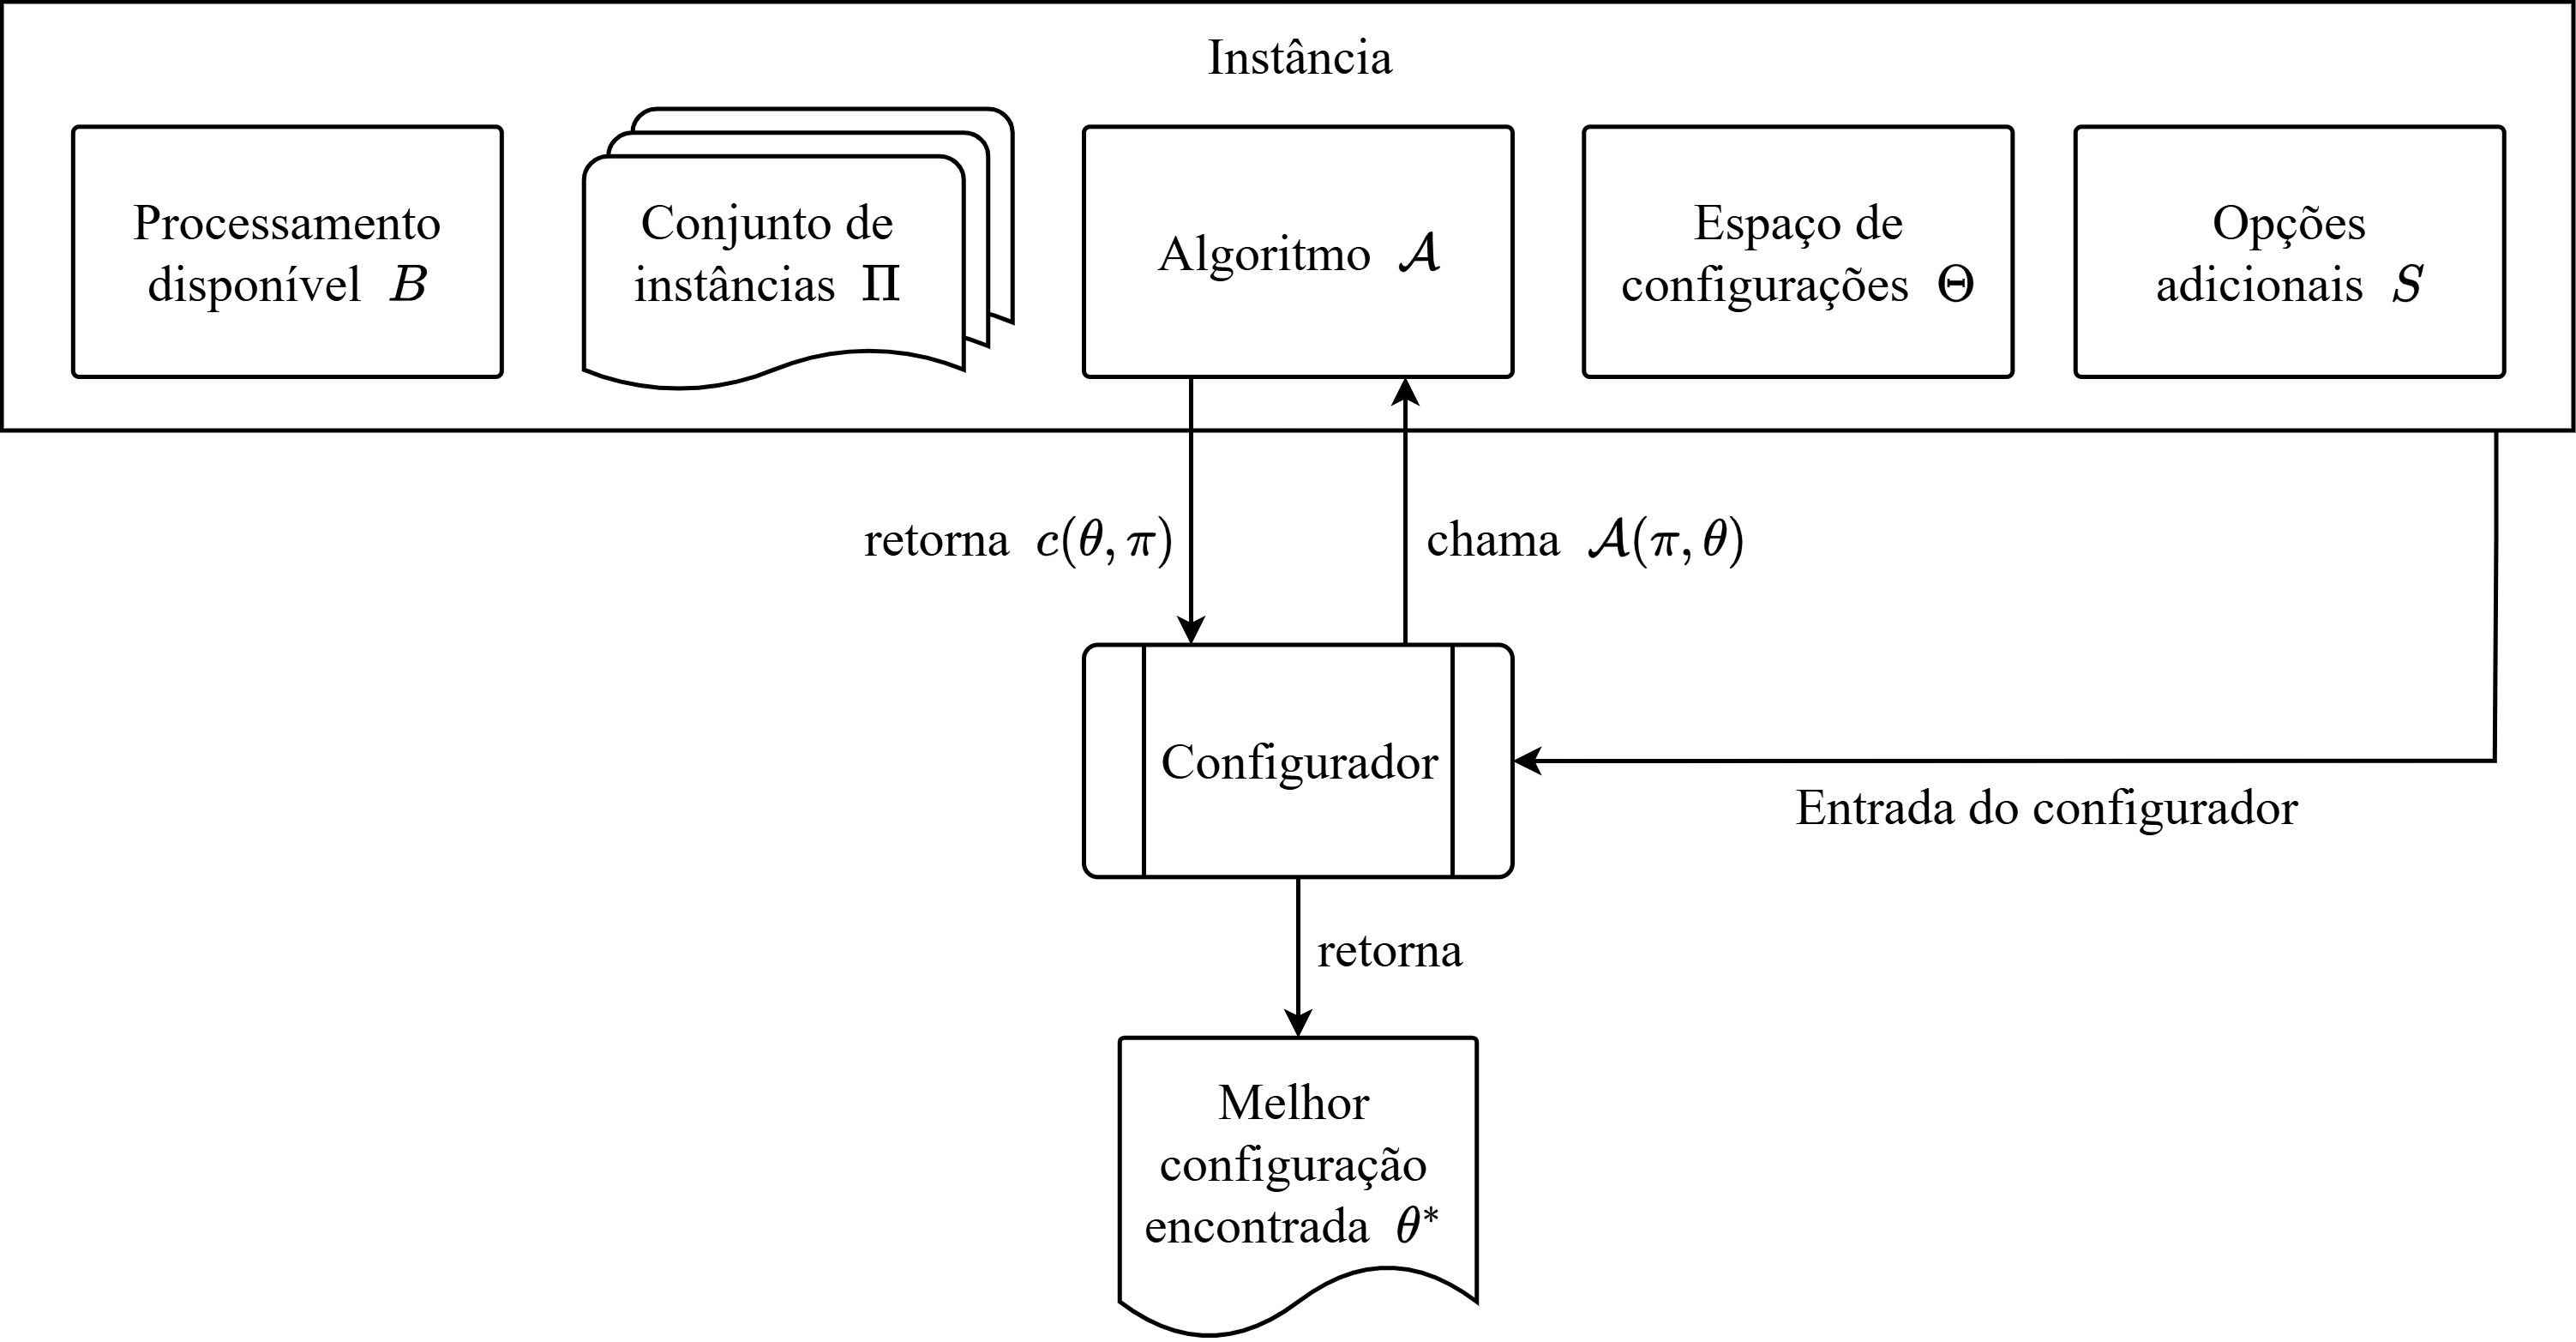
\includegraphics[width=0.85\linewidth]{img/diagrama_configurador.png}
    \caption*{\small \textbf{Fonte:} Adaptado de \cite{souza2022automatic}}
\end{figure}

O processo de \ac{AAC} é desafiador por diversos motivos. O trabalho de \cite{souza2022automatic} organiza esses desafios, identificados durante o desenvolvimento dos diversos configuradores da literatura. Um dos desafios a superar é a dificuldade de obter um conjunto de configurações que otimize a função objetivo para todas as instâncias de treinamento. O configurador precisa avaliar corretamente as métricas de qualidade independentemente da instância para que ele explore corretamente o espaço de soluções. Por exemplo, instâncias com custos de escalas diferentes não podem enviesar o configurador, fazendo-o focar apenas na otimização da instância de maior magnitude.

Outro desafio é a natureza estocástica de certos algoritmos. Nesses casos, podemos precisar de múltiplas execuções do algoritmo alvo para obter uma informação relevante sobre a qualidade de uma configuração. A flexibilidade dos parâmetros também gera dificuldades para o configurador, pois causa interações entre os parâmetros em diferentes magnitudes. O configurador precisa identificar tais interações e utilizar essa informação no processo de busca.

A solução mais óbvia para alguns desses desafios seria realizar mais execuções do algoritmo alvo para obter mais informações. Porém, realizar uma execução é um processo custoso e, devido à limitação de tempo e ao poder de processamento, não devemos desperdiçar execuções. Desta forma, o configurador precisa implementar estratégias que superem esses desafios, minimizando o número de execuções do algoritmo alvo.

Além desses pontos que dificultam a exploração eficiente do espaço de configuração de um algoritmo, o usuário de um configurador também deve levar em conta alguns elementos para extrair todo o potencial dos métodos de \ac{AAC}. Em relação às instâncias que utilizamos no processo, é essencial que façamos uma divisão entre as instâncias de treinamento e teste, pois isso nos permite realizar uma avaliação precisa da efetividade da configuração. Aliado a isso, as instâncias que selecionarmos para o treinamento devem representar as diversas características do restante das instâncias. Essa representatividade garante que o configurador tenha contato com as propriedades das instâncias do problema e, consequentemente, encontre configurações que funcionem bem para as instâncias de teste ou produção \citep{eggensperger2019pitfalls}.

Ainda em relação às instâncias, muitas instâncias difíceis no conjunto de treino farão com que o configurador consuma rapidamente os recursos disponíveis, visto que a maior parte do tempo será gasta pelo algoritmo alvo resolvendo essas instâncias difíceis. Dessa forma, precisamos equilibrar a quantidade de instâncias difíceis no conjunto de treinamento. Esse equilíbrio é crucial, pois, se utilizarmos um conjunto de treino fácil demais, o configurador pode ficar enviesado para instâncias fáceis \citep{eggensperger2019pitfalls}.

O recurso computacional que disponibilizamos ao configurador deve ser coerente com o cenário de configuração. Quanto maior o espaço de configuração, maior deve ser a quantidade de recurso computacional fornecida ao configurador para uma exploração completa do espaço de busca \citep{eggensperger2019pitfalls}. Nesse sentido, o trabalho de \cite{hutter2017configurable} comprova essa afirmação. Ademais, os autores também concluem que, apesar de os configuradores precisarem de poucos recursos para encontrar boas configurações em algoritmos com um espaço de configuração pequeno, dado o tempo e o recurso computacional necessários, a configuração de um algoritmo que possui um grande espaço de configuração gera um ganho relativamente maior.

Ainda no âmbito do espaço de configuração, precisamos escolher bem quais parâmetros de um algoritmo vamos configurar automaticamente e quais serão seus intervalos, pois a adição de poucos parâmetros pode aumentar drasticamente o espaço de configuração. Apesar de a configuração de uma grande quantidade de parâmetros poder gerar uma configuração mais refinada, precisamos considerar o aumento da dificuldade do processo de configuração. Nessa perspectiva, realizar uma configuração de parâmetros cuidadosamente selecionados pode trazer resultados melhores em menos tempo do que tentar configurar todos os parâmetros do algoritmo \citep{eggensperger2019pitfalls}.

\section{Projeto automático de algoritmos}

Até o momento, vimos as características da \ac{AAC}. Explicitamos as motivações para utilizar a \ac{AAC} e os benefícios que essa utilização oferece. Em resumo, essas técnicas nos fornecem uma maneira científica e automatizada de encontrar combinações otimizadas de parâmetros para um algoritmo. Essa automatização auxilia os projetistas de algoritmos na medida em que oferece informações realistas e precisas sobre a efetividade dos componentes que eles desenvolveram. Porém, nesse cenário, a combinação de tais componentes ainda é responsabilidade do projetista. Com isso em mente, uma abordagem mais sofisticada e ambiciosa seria expormos não só os parâmetros do algoritmo para configuração automática, mas também a combinação de diferentes componentes algorítmicos. Logo, todo o processo mecânico do projeto de algoritmos seria realizado de forma automática \citep{stutzle2018automated}. Nesta seção, apresentaremos os conceitos fundamentais do \ac{AAD}.

Primeiramente, demonstraremos a complexidade e as nuances envolvidas no projeto de meta-heurísticas como forma de ilustrar as vantagens no \ac{AAD}. Dessa forma, considere a \ac{ILS} representada no Algoritmo \ref{alg:ils} como exemplo (por simplicidade, o algoritmo não trata explicitamente o armazenamento da melhor solução encontrada, mas assumimos que esse processo ocorre). A \ac{ILS} possui quatro componentes principais: solução inicial, perturbação, melhora e critério de aceitação. Cada uma dessas componentes suporta diversas implementações internas específicas que o projetista deve fazer para obter um algoritmo válido \citep{lourencco2018iterated}. 

% \begin{algorithm}
% \caption{Busca Local Iterada}
% \label{alg:ils}
% \begin{algorithmic}[1]
%     \Ensure
%         $s$: Melhor solução encontrada durante o processo
%     \State $s_0 \gets GeraSolucaoInicial()$ 
%     \State $s^* \gets \operatorname{Melhora}(s_0)$
%     \While{Critério de parada não for atingido}
        
%         \State $s' \gets \operatorname{Perturba(s^*)}$
%         \State $s'' \gets \operatorname{Melhora(s')}$
%         \State $s^* \gets \operatorname{Aceita(s^*, s'')}$
%     \EndWhile
% \end{algorithmic}
% \end{algorithm}

\begin{algorithm}
\caption{Busca Local Iterada}
\label{alg:ils}
\begin{algorithmic}[1]
    \Ensure
        $s$: Melhor solução encontrada durante o processo
    \State $s_0 \gets \texttt{GeraSolucaoInicial}()$ 
    \State $s^* \gets \texttt{Melhora}(s_0)$
    \While{Critério de parada não for atingido}
        
        \State $s' \gets \texttt{Perturba}(s^*)$
        \State $s'' \gets \texttt{Melhora}(s')$
        \State $s^* \gets \texttt{Aceita}(s^*, s'')$
    \EndWhile
\end{algorithmic}
\end{algorithm}

% \begin{algorithm}
% \caption{Busca Local Iterada}
% \label{alg:ils}
% \begin{algorithmic}[1]
%     \Ensure
%         $s$: Melhor solução encontrada durante o processo
%     \State $s_0 \gets \operatorname{Construtiva}()$ 
%     \State $s^* \gets BuscaTabu(s_0)$
%     \While{Critério de parada não for atingido}
        
%         \State $s' \gets AlteracaoAleatoria(s^*)$
%         \State $s'' \gets BuscaLocal(s')$
%         \State $s^* \gets AceitaSempre(s^*, s'')$
%     \EndWhile
% \end{algorithmic}
% \end{algorithm}

Podemos implementar o método \texttt{GeraSolucaoInicial} como, por exemplo, uma heurística construtiva gulosa ou como uma geração aleatória de soluções. Cada uma dessas estratégias possui suas peculiaridades, mas não as abordaremos aqui. Veja \cite{talbi} para uma visão geral das técnicas e \cite{lourencco2018iterated} para um detalhamento das estratégias dentro de uma \ac{ILS}.

Podemos implementar o método \texttt{Perturba} de várias formas. Uma das formas é utilizar as diferentes vizinhanças do problema para modificar soluções. Outra forma é realizar modificações aleatórias em soluções. Esses métodos podem ser combinados de qualquer maneira para gerar perturbações mais sofisticadas, além de que o projetista pode fixar essas combinações ou decidir realizá-las dinamicamente durante a execução. Outro fator é a força das modificações realizadas, isto é, o quão diferentes serão as soluções resultantes. Esse fator pode ser fixo, incrementado quando a busca fica presa em ótimos locais ou o algoritmo pode determiná-lo dinamicamente \citep{stutzle2018automated, lourencco2018iterated}.

Dada uma solução, a tarefa do procedimento \texttt{Melhora} é encontrar um ótimo local e, por isso, ele também é altamente personalizável. Desta forma, podemos utilizar qualquer heurística de busca de solução única para esse fim, incluindo outro procedimento \ac{ILS} \citep{talbi}. Ademais, cada um dos possíveis procedimentos de busca adiciona uma série de decisões de projeto internas, como vizinhanças, regras de comportamento ou simplesmente novos parâmetros numéricos \citep{stutzle2018automated}.

Por fim, o procedimento \texttt{Aceita} varia em um espectro de aceitar apenas soluções que melhoram a função objetivo ou aceitar qualquer nova solução. As opções intermediárias nesse espectro incluem, por exemplo, utilizar modelos probabilísticos como o critério de Metrópolis, que sempre aceita soluções melhores, mas também aceita soluções piores por uma certa probabilidade $\operatorname{exp}((f(s^*)-f(s''))\slash T$ onde $T$ é um parâmetro chamado temperatura. Esse parâmetro pode ser fixo ou variável. No segundo caso, semelhante à meta-heurística \ac{SA}, o projetista deve definir também o esquema de variação da temperatura \citep{lourencco2018iterated}. Para mais detalhes do critério de Metrópolis e \ac{SA} veja \cite{delahaye2018simulated} e \cite{talbi}.

A partir dessa listagem de possibilidades de implementação, concluímos que o processo de implementação de um algoritmo \ac{ILS} efetivo exige que o projetista realize uma exploração manual das diferentes alternativas por meio de testes, intuições sobre o problema-alvo e experiências prévias de outras implementações. Esse trabalho manual possui desvantagens muito parecidas com as desvantagens da configuração manual de parâmetros, ou seja, é um processo dificilmente reprodutível, tedioso, custoso e tende a gerar algoritmos que não utilizam todo o potencial das componentes disponíveis \citep{stutzle2018automated}.

Dessa forma, com o objetivo de mitigar esses problemas, a comunidade científica expandiu os conceitos de \ac{AAC} para automatizar também a exploração do espaço de algoritmos para um determinado problema. Para isso, os componentes algorítmicos, as regras de combinação desses componentes e os parâmetros do algoritmo formam o espaço de configuração. A partir disso, podemos utilizar as técnicas de \ac{AAC} já existentes na exploração deste espaço.

Com isso estabelecido, a responsabilidade do projetista é utilizar sua intuição e conhecimento do problema para desenvolver componentes eficientes. Conforme representado na Figura \ref{img:diagrama_projeto_automatico}, dados esses componentes e as regras para combiná-los, os configuradores podem realizar o processo de combinação automaticamente.

\begin{figure}[h!] 
    \centering
    \caption{Fluxo de um configurador no processo de AAD}
    \label{img:diagrama_projeto_automatico}
    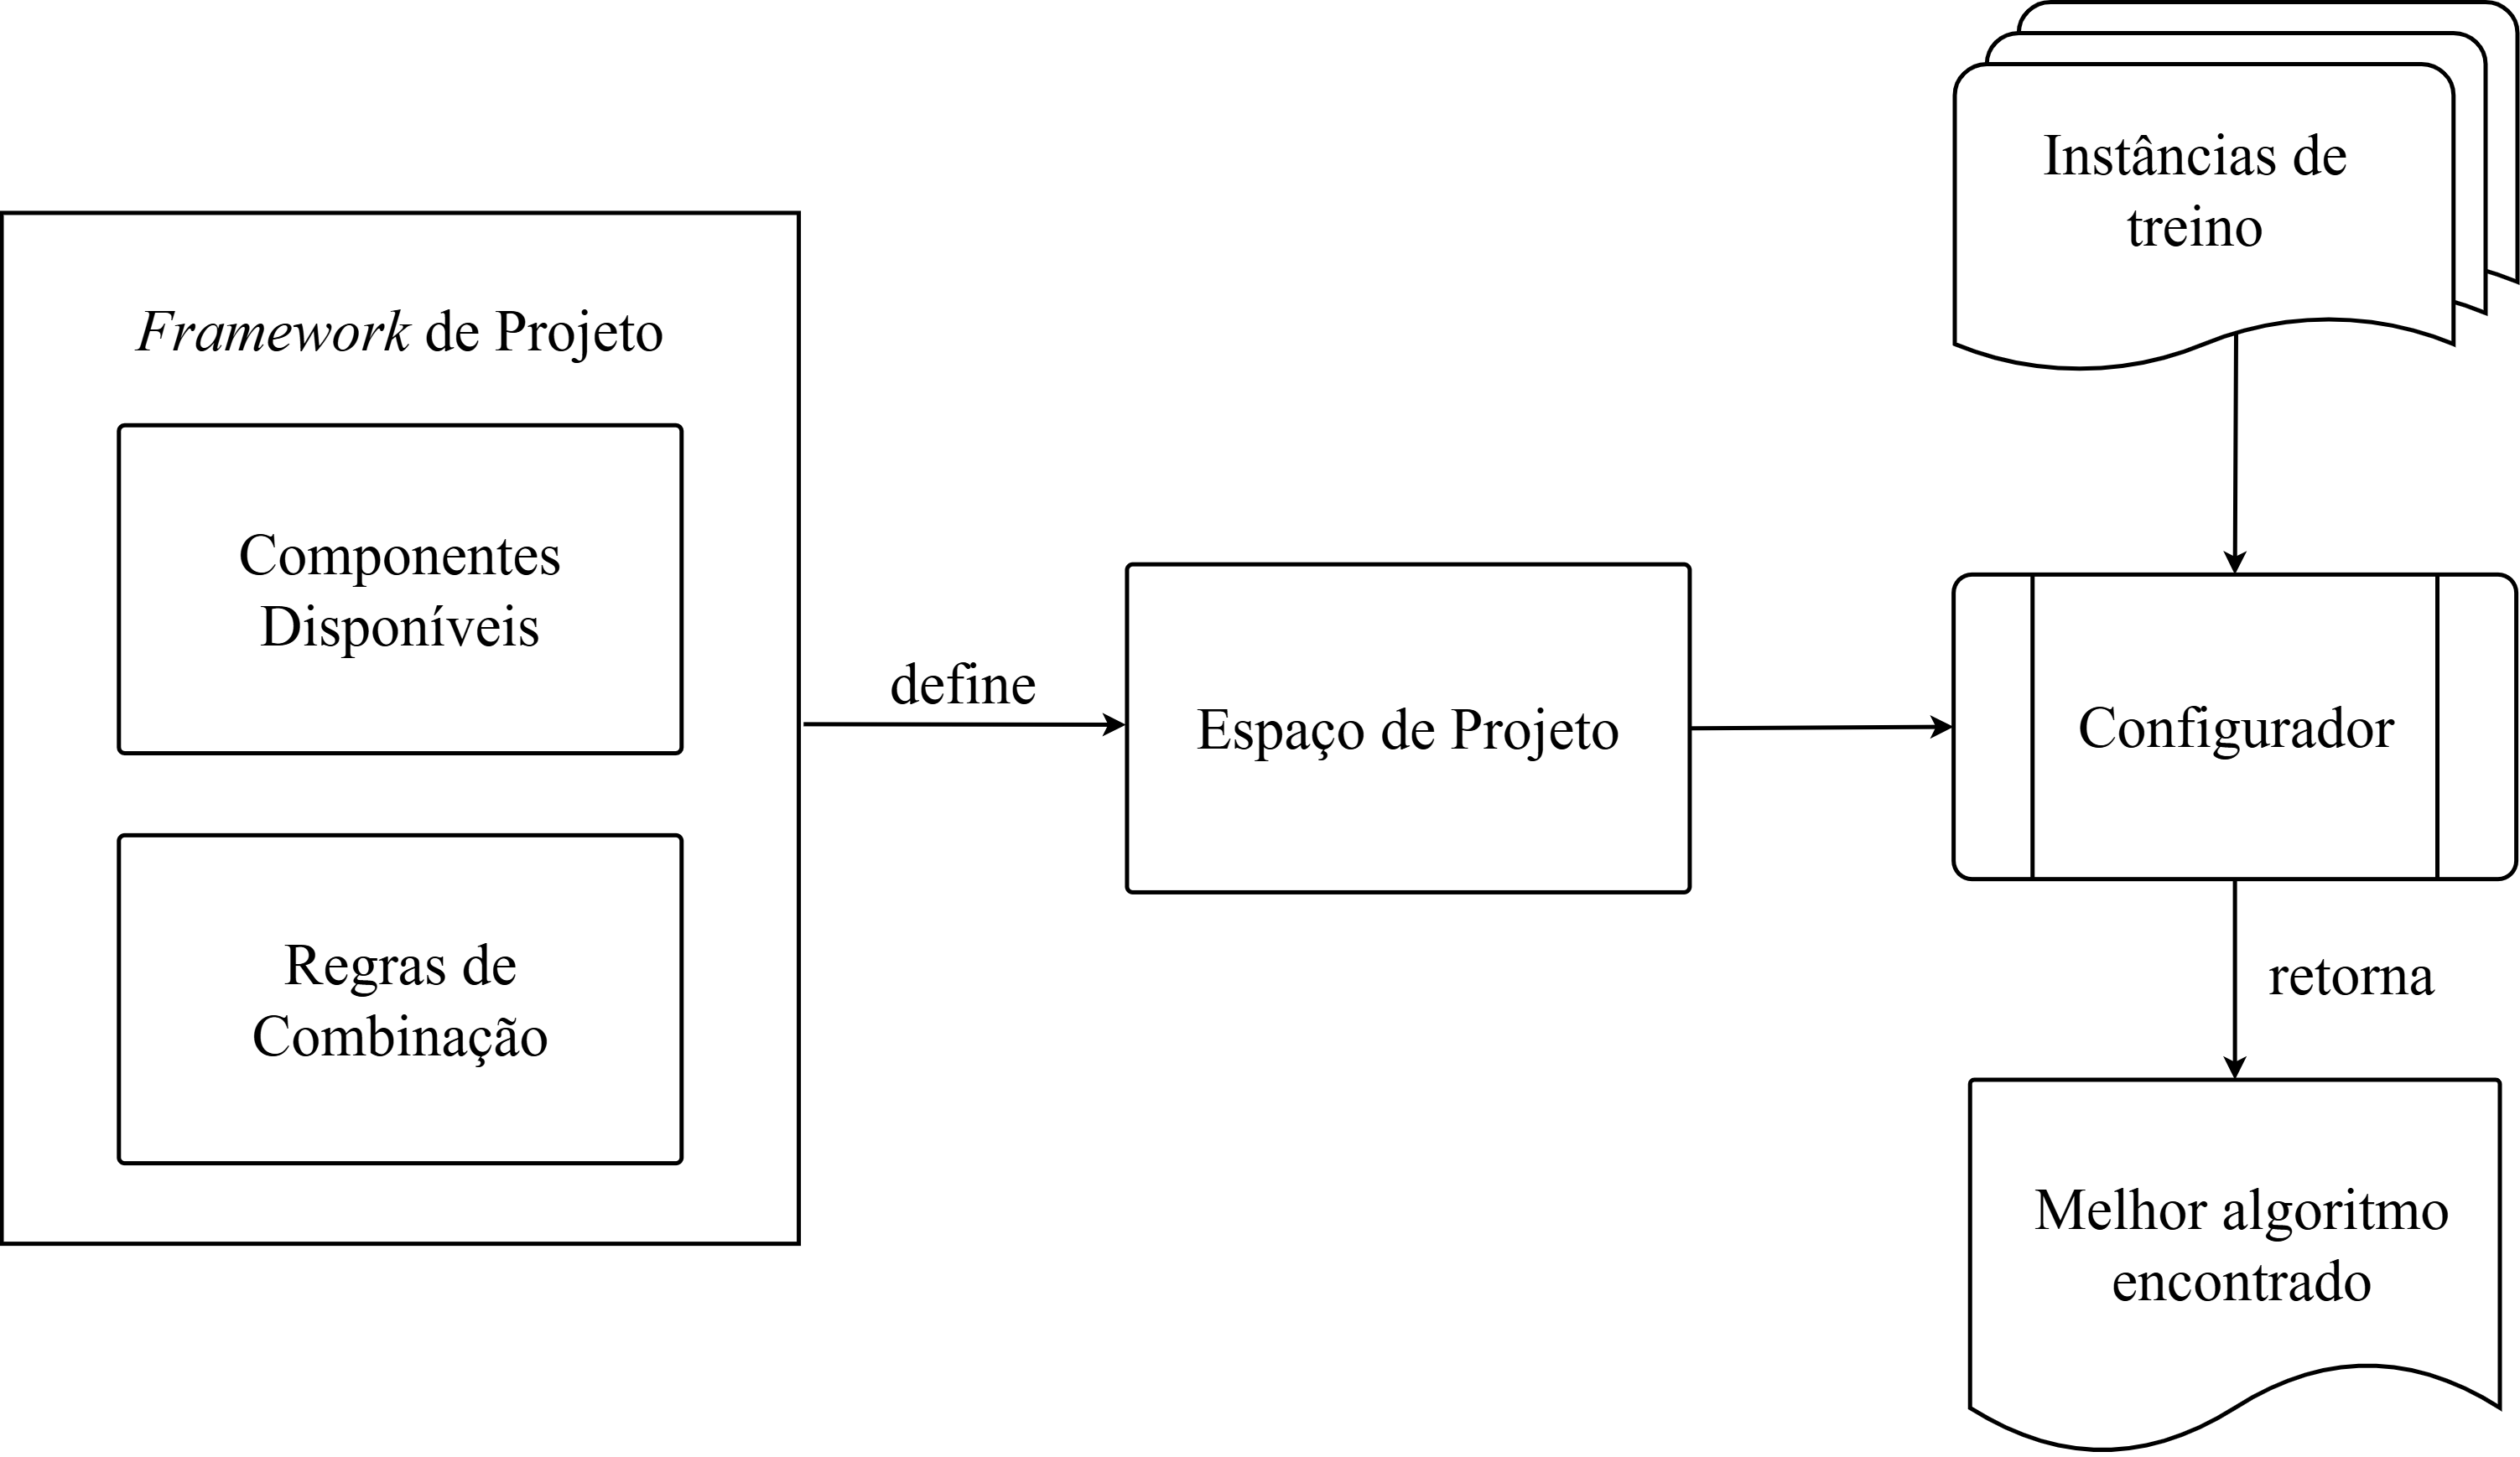
\includegraphics[width=0.60\linewidth]{img/diagrama_projeto_automatico.png}
    \caption*{\small \textbf{Fonte:} Adaptado de \cite{souza2022automatic}}
\end{figure}

\subsection{Abordagem \textit{Top-Down}}\

Uma abordagem \textit{Top-Down}, de forma geral, significa observar o problema do mais alto nível para o mais baixo. Mais especificamente, no contexto do projeto automático de algoritmos, isso significa determinar um modelo de alto nível de um algoritmo e utilizar componentes específicos para instanciar os componentes genéricos desse modelo. Nessa abordagem, o algoritmo resultante sempre terá o formato do modelo definido \citep{mascia2013grammars}. Por exemplo, podemos considerar o Algoritmo \ref{alg:ils} explicado anteriormente como nosso modelo. Recapitulando, precisamos definir quatro componentes para obter um algoritmo de \ac{ILS}: solução inicial, melhoria, perturbação e critério de aceitação. Dessa forma, independentemente de quais componentes específicos escolhermos instanciar, ao final do processo, sempre obteremos uma \ac{ILS}. A Tabela \ref{tab:estrategias_ils} reúne possibilidades de implementação para cada um dos componentes genéricos do modelo.

\begin{table}[h!]
\centering
\caption{Estratégias disponíveis para cada componente da meta-heurística ILS}
\label{tab:estrategias_ils}
\begin{tabular}{lc}
\hline
\textbf{Componente} & \textbf{Estratégias}  \\ 
\hline
Solução Inicial             & \texttt{Construtiva, Aleatória} \\ 
Melhoria                     & \texttt{Busca Tabu, Busca Local, Recozimento Simulado}   \\
Perturbação                 & \texttt{Vizinho Aleatório, Alteração Aleatória}  \\
Critério de Aceitação       & \texttt{Aceita Melhora, Aceita Qualquer, Metrópolis}   \\
\hline
\end{tabular}
    \caption*{\small \textbf{Fonte:} Os Autores.}

\end{table}

A partir da definição dessas componentes específicas, podemos instanciar diferentes algoritmos de \ac{ILS} a partir do modelo. Dessa maneira, podemos buscar as combinações de componentes mais eficientes. No processo de definição dos componentes, precisamos levar em conta que o número de componentes específicas disponíveis afeta diretamente a quantidade de algoritmos que podemos gerar. Por isso, precisamos equilibrar a variabilidade de opções com a complexidade de explorar esse espaço de configuração \citep{souza2022automatic}.

Nesse tipo de abordagem, podemos modelar as regras de combinação dos componentes como parâmetros categóricos de um algoritmo. Por exemplo, poderíamos implementar cada um dos métodos de melhoria e definir um parâmetro categórico $p_i$ que determinaria qual estratégia de melhoria o algoritmo utilizaria na execução de forma que $p_i \in \{\texttt{buscaTabu}, \texttt{buscaLocal}, \texttt{recozimentoSimulado} \}$. Além disso, certas estratégias precisam de parâmetros adicionais; por exemplo, ao instanciarmos a busca tabu como processo de busca, precisamos definir qual vizinhança utilizar e um valor para o parâmetro \textit{tenure}. Podemos modelar esses parâmetros adicionais como parâmetros numéricos ou categóricos condicionais. Dessa forma, a partir dessas ideias, podemos parametrizar as decisões de projeto de algoritmos e utilizar os configuradores já existentes para gerar algoritmos automaticamente. \citep{souza2022automatic} 

Através de trabalhos como \cite{khudabukhsh2016satenstein}, \cite{franzin2019revisiting} e \cite{ bezerra2020automatically}, podemos verificar a efetividade da abordagem \textit{Top-Down} em gerar algoritmos efetivos (veja a Seção \ref{sect:bibconfig} para mais detalhes sobre os trabalhos da literatura de \ac{AAC} e \ac{AAD}). Porém, para utilizá-la eficientemente, precisamos determinar previamente o modelo do algoritmo e considerar as possíveis interações entre cada um dos componentes implementados. Essa tarefa se torna mais difícil à medida que o número de componentes cresce \citep{mascia2014grammar}. Por esse motivo, podemos utilizar, alternativamente, a estratégia \textit{Bottom-Up} para automatizar o processo de desenvolvimento de algoritmos de forma mais flexível.

% A figura \ref{img:algoritmos_ils_instanciados} mostra dois exemplos de possíveis algoritmos \ac{ILS} gerados. Podemos observar que cada um deles utiliza combinações totalmente diferentes de componentes, de forma que eles obteriam resultados diferentes ao executar as instâncias de treinamento.

% \begin{figure}[h!] 
%     \centering
%     \caption{Possíveis algoritmos ILS gerados com a abordagem \textit{Top-Down} de projeto automático de algoritmos}
%     \label{img:algoritmos_ils_instanciados}
%     \includegraphics[width=0.85\linewidth]{img/algoritmos_ils_instanciados.png}
% \end{figure}



\subsection{Abordagem \textit{Bottom-Up}} \label{sect:bottomup}

A abordagem \textit{Bottom-Up} nos permite focar no desenvolvimento dos componentes algorítmicos sem precisarmos determinar o formato do algoritmo final. Além de simplificar algumas fases do processo, essa abordagem tende a gerar algoritmos totalmente novos e híbridos.

Apesar da flexibilidade na geração de algoritmos, ainda precisamos definir as regras de combinação dos componentes. Uma das formas de representar esse cenário é utilizando uma gramática livre de contexto na forma Backus-Naur. Definimos essa gramática de forma que qualquer derivação das regras gere um algoritmo válido \citep{mascia2013grammars}. Na Figura \ref{img:gram_backus_exemplo} podemos ver um exemplo de gramática capaz de gerar algoritmos compostos por diferentes combinações de componentes. Para a definição e teoria em gramáticas livres de contexto, veja \cite{papadimitriou1997elements}.

\begin{figure}[h!] 
    \centering
    \caption{Gramática livre de contexto na forma Backus-Naur para geração de um algoritmo de busca}
    \label{img:gram_backus_exemplo}
    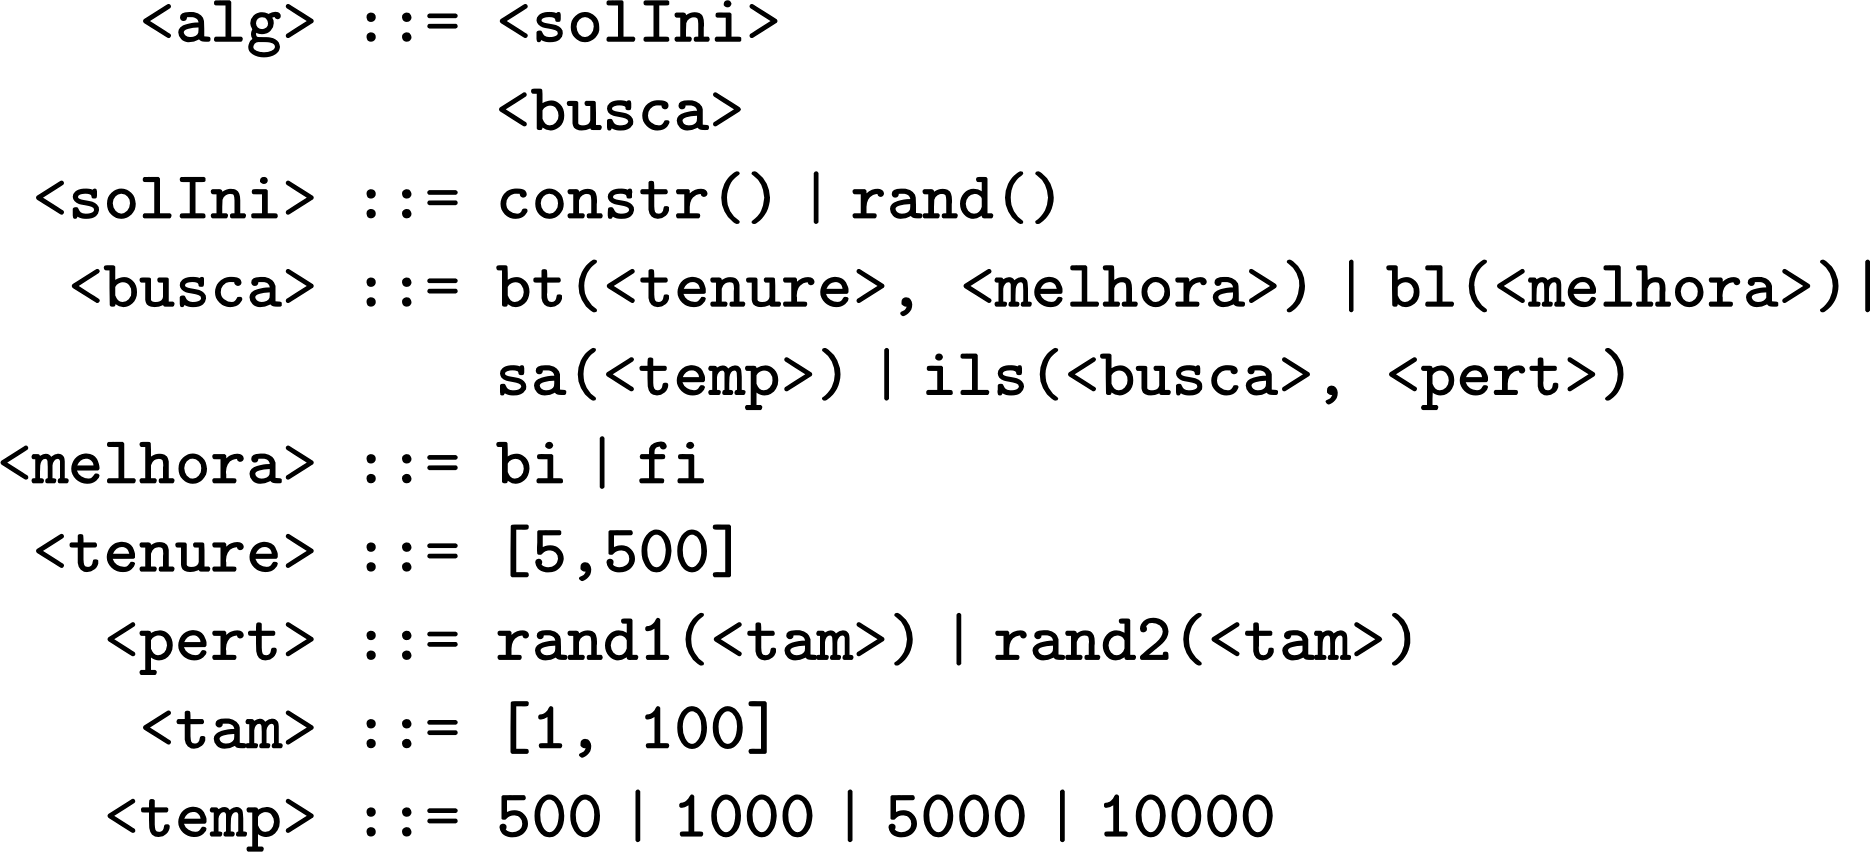
\includegraphics[width=0.75\linewidth]{img/gram_backus_exemplo.png}
    \caption*{\small \textbf{Fonte:} Os Autores.}
\end{figure}

A gramática é composta por uma série de regras de transformação de símbolos não terminais. A forma Backus-Naur representa os símbolos não terminais entre os caracteres \texttt{<>}. Cada regra define uma escolha de projeto. Por exemplo, o símbolo inicial da gramática de exemplo é o \texttt{<alg>}. Esse símbolo deriva para os não terminais de solução inicial \texttt{<solIni>} e processo de busca \texttt{<busca>}, indicando que esses componentes devem existir no algoritmo. O primeiro símbolo deriva para algumas estratégias de gerar soluções iniciais, enquanto o segundo tem o potencial de gerar métodos de busca inteiros sofisticados e híbridos. Cada um dos métodos de busca $\texttt{bt}$ (Busca Tabu), $\texttt{bl}$ (Busca Local), $\texttt{sa}$ (\textit{Simulated Annealing}) e $\texttt{ils}$ (Busca Local Iterada) possui seus próprios argumentos, os quais outros símbolos não terminais determinam; inclusive, um deles recebe outro método de busca como argumento, gerando recursividade na gramática.

Podemos notar que os símbolos não terminais da gramática derivam ou para um conjunto determinado de valores ou para um intervalo numérico específico. A partir dessa percepção, \cite{mascia2013grammars} propôs mapear os símbolos não terminais para parâmetros categóricos ou numéricos em um algoritmo e, com isso, utilizar técnicas de \ac{AAC} para realizar a derivação da gramática. Dessa forma, um símbolo não terminal que deriva de outro símbolo não terminal se torna um parâmetro condicional em relação ao parâmetro do símbolo gerador. Também precisamos tratar da recursividade da gramática, visto que um algoritmo possui um conjunto finito de parâmetros. \cite{mascia2013grammars} propõe criar cópias dos parâmetros para cada nível permitido de recursão, de forma que os parâmetros do nível $i+i$ sejam condicionais ao parâmetro que gera a recursão no nível $i$.
 

% \section{Teoria de Complexidade}é capaz 

% Entender conceitos de complexidade de algoritmos e de problemas é essencial quando se busca soluções para problemas, no sentido de que essas ferramentas permitem avaliar a viabilidade de uma solução a partir do seu consumo de tempo e espaço. Esta seção expõe formas de medir o tempo de execução de algoritmos e formas de classificar problemas pela sua complexidade inerente.

% \subsection{Complexidade de Algoritmos}

% O tempo de execução de um algoritmo em uma máquina é influenciado por diversos fatores, como sistema operacional da máquina, tarefas concorrentes na máquina, dados de entrada, linguagem de programação, bibliotecas e compilador utilizados para implementação, entre outros. Além disso, execuções de algoritmos com exatamente os mesmos parâmetros em uma mesma máquina podem levar tempos diferentes para finalizar. Por isso, existem padronizações para medir a eficiência de um algoritmo. Na maioria dos casos, essa eficiência é medida no número de passos que o algoritmo leva para resolver um problema e em função do tamanho da entrada dada ao algoritmo, ou seja, a partir do momento em que a definição da função que representa o tempo de execução do algoritmo é feita, é possível prever quanto tempo ele levaria com um novo tamanho de entrada \citep{cormen2022introduction}.

% Ainda assim, expressões que definem exatamente o tempo de execução de um algoritmo tendem a ser complexas. Por isso, é mais conveniente expressar o tempo de execução através de uma estimativa. Essa estimativa é chamada de notação assintótica e consiste em considerar apenas o termo de maior ordem da expressão, ignorando fatores constantes que afetam o tempo de execução do algoritmo. Essa abordagem estabelece um limite superior do crescimento do tempo de execução em relação ao tamanho da entrada dada ao algoritmo. Com isso, é possível expressar a complexidade de um algoritmo de forma simples, mas sem causar perda de informação que possa resultar em erros de análise e de comparação entre algoritmos \citep{sipser2013introduction}.

% A exemplo, considere que a função \(f(n) = 3n^5+7n^4+n^{1/2}\) representa o tempo de execução de um algoritmo $A$. Podemos declarar que o tempo de execução assintótico desse algoritmo é $O(n^5)$, isto é, os termos de menor ordem são descartados juntamente com os fatores constantes. Com isso, temos que, independentemente de quaisquer fatores, o tempo de execução do algoritmo $A$ tem um grau de crescimento menor ou igual a $n^5$.

% No começo do estudo de complexidade de problemas, houve certo progresso em provar que alguns problemas não podem ser resolvidos em tempo polinomial, mas, para muitos problemas fundamentais, essa questão permanece sem resposta. Por isso, além de não conhecermos algoritmos polinomiais para tais problemas, também não podemos provar que eles não existam \citep{eva2005}.

% Dessa forma, podemos introduzir o conceito de verificadores polinomiais. Um algoritmo $A$ é um verificador válido de um problema $X$ se recebe como argumentos $I$ e $c$, executa em tempo polinomial e, além disso, para todas as instâncias $I$ do problema $X$ que respondem "sim", existe um polinômio $p$ tal que existe algum certificado $c$, de forma que $|c| \leq p(|I|)$, para o qual $A$ responde "sim". Com isso, podemos definir a classe de problemas que possuem algum verificador polinomial válido. Ela é chamada de $NP$ \citep{eva2005}.

% Por exemplo, seja $X$ o problema de, dado um grafo simples $G=(V,E)$, verificar se existe um caminho hamiltoniano em $G$. Com isso, seja $A$ um algoritmo que recebe como argumentos um grafo simples como instância de $X$ e um certificado $c$ igual a uma sequência de vértices de $G$ que formam um suposto caminho hamiltoniano. O algoritmo verifica se $|c|=|V|$, verifica se todos os vértices de $G$ estão contidos em $c$ e, para cada $v_i \in c$, verifica se existe a aresta $\{v_i, v_{i+1}\}$ em $G$. Podemos verificar que o algoritmo claramente executa em tempo polinomial pois, respectivamente, cada passo descrito leva tempo $O(|V|)$, $O(|V|^2)$ e $O(|V|*|M|)$. Além disso, se $G$ possui um caminho hamiltoniano, sempre existe um certificado $c$, o próprio caminho hamiltoniano, de forma que $|c|=|V|$, que faz o verificador descrito responder "sim". Portanto, $A$ é um verificador válido para $X$ e, consequentemente, $X$ está em $NP$ como já demonstrado por \cite{garey1976complexity}.

% As definições das classes $P$ e $NP$ geram a consequência de que $P \subseteq NP$. Seja $X$ um problema qualquer da classe $P$. Ademais, seja $A$ um algoritmo polinomial que resolve $X$. Com isso, definimos o algoritmo $B$ que, dada uma instância $I$ de $X$ e um certificado $c$, utiliza o algoritmo $A$ internamente para resolver a instância $I$ e devolve a resposta de $A$ como sua resposta. Podemos verificar que, se $A$ resolve $X$, o algoritmo $B$ responde "sim" se e somente se $I$ é uma instância "sim". Além disso, o certificado $c$ não importa na verificação e, como $A$ é polinomial, $B$ também é. Portanto, podemos concluir que todos os problemas de $P$ possuem um verificador válido e, com isso, temos que $P \subseteq NP$ \citep{eva2005}.



% Outro conceito que precisamos introduzir é a redução polinomial entre dois problemas. Dados dois problemas $A$ e $B$, reduzir o problema $A$ para o problema $B$ significa definirmos uma função $f$ que mapeia todas as instâncias de $A$ para instâncias de $B$. O mapeamento deve funcionar de forma que, para qualquer instância de $A$, $I_A$, a sua imagem $f(I_A)$ responde "sim" para o problema $B$ se e somente se $I_A$ responde "sim" para o problema $A$. Em outras palavras, se uma redução de $A$ para $B$ existe, podemos utilizar um algoritmo que resolve $B$ para resolver $A$ através da redução das instâncias de $A$. Uma redução polinomial entre dois problemas $A$ e $B$, escrita $A \leq_p B$, é uma redução que pode ser computada em tempo polinomial \citep{eva2005}.

% Uma consequência da definição de redução polinomial é que se existe uma redução polinomial $A \leq_pB$ e existe um algoritmo que resolve $B$ em tempo polinomial, então $A$ também pode ser resolvido em tempo polinomial. Perceba que, dada a instância $I_A$ de $A$, basta realizar a redução que leva tempo polinomial e executar o algoritmo polinomial do problema $B$ sobre a instância $f(I_A)$. Dessa forma, a composição das duas fases polinomiais gera um algoritmo polinomial que resolve $A$.

% A definição de reduções polinomiais nos permite apresentar outra classe de problemas. Os problemas NP-Difíceis. Um problema $X$ é NP-Difícil se, para cada problema $Y$ da classe $NP$ existe uma redução polinomial $X \leq_pY$. Por conta dessa definição, caso algum pesquisador encontre um algoritmo polinomial para qualquer problema NP-Difícil, todos os problemas de NP serão resolvíveis em tempo polinomial implicando em $P=NP$.

% \section{Métodos Heurísticos(TODO:adicionar pseudocódigos de exemplo}



% Entender o funcionamento de diferentes métodos heurísticos é importante para este trabalho por dois motivos principais. Primeiramente, precisamos compreender as estratégias para que, a partir disso, possamos combiná-las utilizando técnicas de configuração automática. Ademais, visto que o objetivo das técnicas de configuração automática é automatizar a combinação de componentes heurísticos, precisamos entender as componentes para verificar o ganho proporcionado por essas técnicas. Esta seção aborda conceitos básicos de heurísticas e meta-heurísticas através da definição de vizinhança e detalhamento dos principais métodos heurísticos que serão úteis ao escopo deste trabalho.

% \subsection{Vizinhanças}

% Dado o conjunto de todas as soluções de um problema $S$, \cite{talbi} define uma vizinhança como um mapeamento de cada solução $s \in S$ para um subconjunto de soluções $N(s) \subseteq S$. Chamamos de vizinha de $s$ uma solução $s' \in N(s)$. O mapeamento da vizinhança modifica soluções sistematicamente para gerar novas soluções. Por isso, a vizinhança é uma componente específica ao problema-alvo, isto é, sua forma e eficiência dependem exclusivamente de características do problema. Isso é verdade pois modificar uma solução inclui manipular a representação da solução, representação essa que varia entre problemas e até mesmo entre diferentes abordagens sobre o mesmo problema \citep{talbi}.

% O autor de uma vizinhança deve considerar algumas características durante o desenvolvimento. Uma delas é a localidade da vizinhança; essa propriedade consiste no impacto que alterações na representação de uma solução têm sobre a qualidade da solução. Se pequenas alterações na representação causam pequenas mudanças na solução, a vizinhança possui baixa localidade. Por outro lado, se pequenas alterações na representação causam grandes mudanças na solução, a vizinhança possui alta localidade. Nesse sentido, uma exploração do espaço de busca por meio de uma vizinhança com baixa localidade é mais significativa \citep{talbi}.

% Outro ponto importante é o tamanho da vizinhança. Gerar e explorar uma vizinhança muito grande pode ter um custo muito alto e, com isso, atrapalhar o processo de busca. Por outro lado, vizinhanças muito restritas e, consequentemente, pequenas, podem ignorar soluções promissoras no espaço de soluções. \citep{talbi}.

% A partir deste ponto, precisamos introduzir uma maneira de quantificar a qualidade de uma solução chamada de função objetivo. Essa função mapeia todo o conjunto de soluções $S$ de um problema para valores reais, $f : S \to \mathbb{R}$. Essa ferramenta permite comparar soluções pela sua qualidade \citep{talbi}. Além disso, o presente trabalho trata apenas de problemas de minimização, isto é, quanto menor é o custo de uma solução, melhor é a solução. Por isso, por conveniência, em qualquer contexto, sendo $s_1$ e $s_2$ soluções para um dado problema, $f(s_1) < f(s_2)$ significará que a solução $s_1$ é melhor que a solução $s_2$.

% Com o conceito de vizinhança estabelecido, podemos introduzir o conceito de ótimo local. Esse conceito é importante pois diversas meta-heurísticas mais sofisticadas implementam múltiplas técnicas para evitar ótimos locais. \cite{talbi} define um ótimo local como uma solução $s'$ tal que não existe nenhuma solução $s''$ na vizinhança $N(s')$ que $f(s'') < f(s')$. Um ótimo global, por sua vez, além de também ser um ótimo local, é uma solução $s'$ que, para qualquer solução $s''$ do espaço de busca, $f(s') \leq f(s'')$ \citep{talbi}. A Imagem 1(TODO: FAZER GRÁFICO DE MÍNIMOS LOCAIS) apresenta um gráfico que representa os valores $f$ pelo espaço de busca e indica ótimos locais e ótimos globais.

% \subsection{Busca Local}

% A busca local é uma das meta-heurísticas mais básicas e, por isso, meta-heurísticas mais sofisticadas utilizam seus conceitos internamente. Dada uma solução inicial $s_0$, a cada iteração $i$, a busca local gera a vizinhança $N(s_i)$ da solução $s_i$. Com isso, a busca local seleciona uma solução $s_{i+1} \in N(s_i)$ tal que $f(s_{i+1}) < f(s_i)$, em outras palavras, seleciona uma solução que melhora a função objetivo. Por fim, o algoritmo finaliza o processo de busca quando não existe nenhuma solução $s' \in N(s_i)$ de forma que $f(s') < f(s_i)$. Por esse motivo, a busca local não consegue escapar de ótimos locais no espaço de busca \citep{talbi}.

% Podemos realizar a exploração do espaço de busca e a seleção de vizinhos na busca local de diferentes formas. Uma delas, a seleção por melhor melhora, consiste em selecionar o melhor vizinho de uma solução a cada iteração, isto é, tendo uma solução $s_i$, o algoritmo seleciona a vizinha de $s_i$ que oferece o máximo de melhoria na função objetivo em relação a $f(s_i)$. Utilizar esse tipo de seleção significa gerar e avaliar todos os vizinhos da solução a cada iteração. Esse processo pode ter um custo elevado em vizinhanças grandes \citep{talbi}.

% \begin{algorithm}
% \caption{Busca Local}
% \label{alg:busca_local}
% \begin{algorithmic}[1]
%     \Require
%         \State $s_0$ \Comment{Solução inicial}
%         \State $N$ \Comment{Estrutura de vizinhança}
%     \Ensure
%     \State $s \gets s_0$ \Comment{Gera uma solução inicial aleatória ou por heurística.}
%     \State $houveMelhora \gets \text{verdadeiro}$
    
%     \While{$houveMelhora$}
%         \State $houveMelhora \gets \text{falso}$
%         \State $s_{melhor\_vizinho} \gets \Call{BuscarMelhorVizinho}{N(s_{atual})}$ \Comment{Encontra o melhor vizinho na vizinhança $N(s_{atual})$.}
        
%         \If{$f(s_{melhor\_vizinho}) < f(s_{atual})$}
%             \State $s_{atual} \gets s_{melhor\_vizinho}$ \Comment{Atualiza a solução atual se o vizinho for melhor.}
%             \State $houveMelhora \gets \text{verdadeiro}$ \Comment{Sinaliza que a busca deve continuar.}
%         \EndIf
%     \EndWhile
    
%     \State \Return $s_{atual}$ \Comment{Retorna o ótimo local encontrado.}
% \end{algorithmic}
% \end{algorithm}

% Outra forma de selecionar vizinhos consiste em selecionar o primeiro vizinho de $s_i$ que melhora a função objetivo. Por isso, ao contrário da primeira opção, o algoritmo não precisa gerar e avaliar toda a vizinhança. Isso gera uma exploração do espaço de busca mais rápida; porém, corre-se o risco de que o processo ignore boas soluções simplesmente pela ordem de geração e avaliação dos vizinhos. Chamamos essa segunda estratégia de seleção por primeira melhora \citep{talbi}.

% O maior problema de uma busca local simples é a incapacidade de escapar de ótimos locais. Por esse motivo, buscas locais tendem a finalizar o processo de busca precocemente e sem realizar uma exploração satisfatória no espaço de busca \citep{talbi}. Nesse sentido, as próximas meta-heurísticas que abordaremos focam em implementar diferentes estratégias para sair de ótimos locais. 

% \subsection{Busca Tabu}

% A busca tabu é semelhante à busca local no sentido de que inicia a busca a partir de uma solução inicial $s_0$ e explora o espaço de busca iterativamente, selecionando novas soluções que melhoram a função objetivo. Porém, a busca tabu não encerra a busca ao chegar em um ótimo local no espaço de busca. Ao invés disso, a busca seleciona uma solução que piora a função objetivo para escapar do ótimo local. Nesse sentido, ela seleciona o vizinho com menor valor de função objetivo, mesmo que ele não seja melhor que a solução que o gerou \citep{talbi}.

% % Durante a exploração do espaço de soluções na busca local, a solução da iteração atual é sempre melhor que todas as soluções de iterações anteriores. Por outro lado,
% Diferentemente da busca local, a busca tabu, ao selecionar soluções que pioram a função objetivo, permite que soluções selecionadas em iterações anteriores sejam melhores que a solução da iteração atual. Por isso, é intuitivo pensar que a busca pode ficar presa em um ciclo infinito de pioras e melhoras da função objetivo. Porém, a busca tabu utiliza uma memória para evitar selecionar soluções repetidas. Ela implementa essa memória em uma lista tabu que armazena informação sobre soluções anteriormente acessadas e, com essa informação, não reexplora soluções \citep{talbi}.

% A implementação da lista tabu depende de características específicas do problema-alvo. Armazenar as soluções integralmente nem sempre é viável pelo espaço de armazenamento necessário e pelo custo de verificar se uma solução está na lista. Por isso, em certos problemas, é mais vantajoso armazenar uma informação parcial das soluções e, com isso, ganhar eficiência de verificação da lista em detrimento da precisão de verificação \citep{talbi}.
% % Por exemplo, podemos implementar a lista tabu de forma que ela armazene os movimentos que o algoritmo realizou na solução entre cada iteração e barrar novas soluções que revertam esses movimentos. Essa estratégia torna eficiente verificar se a lista tabu permite um movimento, mas não impede que o algoritmo selecione soluções repetidas, visto que, em certos problemas, é possível retornar à mesma solução por diferentes sequências de modificações \citep{talbi}.  

% \subsection{Busca Local Iterada}

% % Ao analisarmos o comportamento de uma busca local, observamos que 
% O resultado que a busca local obtém depende da solução inicial utilizada, pois cada solução inicial está associada a um número limitado de ótimos locais. Nesse sentido, a busca local iterada (ILS) realiza, iterativamente, buscas locais com diferentes soluções iniciais para encontrar diferentes ótimos locais. Porém, para realizar uma exploração mais significativa do espaço de busca, a ILS utiliza como solução inicial, em cada iteração, uma perturbação do ótimo local encontrado na iteração anterior. Dado que um ótimo local possui características de uma boa solução, pode ser mais vantajoso continuar a busca a partir dos seus vizinhos ao invés de voltar para uma solução aleatória \citep{talbi}.
% % Essa estratégia é baseada na ideia de que, sendo o ótimo local a melhor solução em uma certa área do espaço de busca, ele possui características de uma boa solução e, por isso, devemos manter algumas delas para alcançar outra boa solução \citep{talbi}.

% Algumas características da ILS incluem a possibilidade de utilizar qualquer heurística de solução única como método de busca, isto é, o processo de encontrar um ótimo local a cada iteração é uma caixa-preta para a ILS no sentido de que essa caixa-preta deve receber uma solução e encontrar um ótimo local \citep{talbi}.

% Além disso, o processo de perturbação do ótimo local é outro componente importante para a ILS. Esse procedimento tem como objetivo afastar o processo de busca dos ótimos locais encontrados em cada iteração. O impacto da perturbação na solução pode variar a depender da estratégia. Por exemplo, quando o processo de busca utilizado é altamente eficiente, realizar uma pequena modificação na solução fará com que o processo de busca encontre o mesmo ótimo local na próxima iteração, fazendo a ILS ficar presa em um ciclo \citep{talbi}.

% Por fim, após realizar a perturbação e o processo de busca sobre o ótimo local perturbado, a ILS utiliza, na próxima iteração, o novo ótimo local encontrado pela heurística de busca apenas se ele passar em um critério pré-determinado. Esse critério varia em um espectro no qual um dos extremos é aceitar apenas soluções que melhoram a função objetivo e o outro extremo é aceitar soluções independentemente de seus valores na função objetivo. Ao utilizarmos uma ILS para resolver um problema, é importante encontrarmos um ponto nesse espectro que seja adequado às particularidades do problema-alvo \citep{talbi}.

% \subsection{\textit{Variable Neighborhood Search}}

% A meta-heurística de busca em vizinhança variável (\textit{Variabel Neighborhood Search} - \ac{VNS}) se apoia na ideia de que diferentes vizinhanças de um mesmo problema exploram subespaços de busca diferentes. Nesse sentido, a estratégia consiste em explorar o espaço de busca utilizando um conjunto predefinido de diferentes vizinhanças para evitar e escapar de ótimos locais \citep{talbi}.

% Mais especificamente, podemos dividir o processo de busca na \ac{VNS} em três fases: \textit{Shake}, busca local e \textit{move}. Dada uma lista de estruturas de vizinhança $N = \{N_1, N_2,...N_{n-1}, N_n\}$, a cada iteração, a \ac{VNS} realiza o \textit{shake} de uma solução inicial $s$ pela vizinhança atual $N_k \in N$, isto é, o algoritmo seleciona uma solução $s'$ aleatoriamente da vizinhança $N_k(s)$. Após o \textit{shake}, a \ac{VNS} aplica um processo de busca local sobre a solução $s'$, encontrando um ótimo local $s''$. Por fim, caso $f(s'') < f(s)$, o \ac{VNS} realiza o \textit{move}, ou seja, seleciona $s''$ para a próxima iteração e redefine $k=1$; caso contrário, o algoritmo repete todo o processo utilizando a solução $s$ com $k = k+1$ \citep{talbi}.

% \subsection{Algoritmos Evolutivos}

% Todas as meta-heurísticas abordadas anteriormente trabalham apenas com uma solução a cada iteração, isto é, esses processos de busca observam o resto do espaço de busca a partir de uma única solução. Ao caracterizarmos estratégias por esse ponto de vista, podemos observar um outro tipo de método de busca que trabalha com um conjunto de soluções a cada momento. Chamamos esses métodos de heurísticas de população no sentido de que uma população se refere a um conjunto definido de soluções \citep{talbi}.

% Dentro da classe de heurísticas de população existem os algoritmos evolutivos. Esses métodos heurísticos se baseiam na competição entre soluções de forma a simular a evolução de espécies. Nesse sentido, também são caracterizados pela sua potencial complexidade ao serem aplicados em problemas de otimização \citep{talbi}. Esta seção não tem como objetivo detalhar todos os pormenores das técnicas utilizadas na computação evolutiva. Nesse sentido, o objetivo é estabelecer conceitos básicos que serão úteis ao entendimento de técnicas que serão posteriormente citadas.

% Algoritmos evolutivos se dividem em fases que, geralmente, são comuns a quase todas as suas subclasses. Inicialmente, o algoritmo gera uma população inicial. Tal processo é feito de forma aleatória ou por meio de alguma estratégia específica. Além disso, também temos uma função objetivo que determina a qualidade de cada solução. A partir da população gerada, o algoritmo seleciona alguns indivíduos para serem os pais das novas soluções. Os critérios de seleção podem variar, mas a estratégia mais comum é que soluções com melhor qualidade tenham maior probabilidade de serem selecionadas \citep{talbi}.

% Em seguida, o algoritmo reproduz os indivíduos selecionados de forma a gerar soluções filhas. As técnicas mais comuns para isso incluem \textit{crossover} e mutação de indivíduos. O algoritmo, então, realiza um processo de substituição para selecionar subconjuntos dos indivíduos pais e filhos para formarem a população da próxima iteração. Por fim, chamamos todo esse processo de geração e podemos vê-lo, na prática, como uma iteração de um algoritmo evolutivo \citep{talbi}.

% \section{Grafos}



% A estrutura de um grafo suporta diversas modelagens de conceitos do mundo real. Entender essa estrutura não só capacita o indivíduo a criar modelos que representam conceitos reais, mas também permite manipular e utilizar esses modelos em prol da resolução de problemas. Esta seção explica conceitos da teoria de grafos que serão úteis ao escopo deste trabalho.

% \subsection{Grafo Acíclico Direcionado}

% \subsection{Ordenação Topológica}


\chapter{Trabalhos Relacionados} \label{chapt:trabalhos}

O \ac{JITJSS} foi proposto pela primeira vez em 2008 por \cite{baptiste2008lagrangian}. Desde então, diferentes autores estudaram o problema e propuseram diferentes estratégias para resolvê-lo. Nesta seção, listaremos com detalhes os trabalhos que abordaram o problema. Além disso, ainda não há nenhum trabalho que aplicou as técnicas de \ac{AAD} especificamente ao \ac{JITJSS}. Por isso, como forma de justificar este trabalho, apresentaremos os usos de \ac{AAC} e \ac{AAD} da literatura para encontrar algoritmos estado da arte para diversos problemas. 
 
\section{\textit{Just-In-Time Job Shop}} \label{sect:bibjitjsp}

\cite{baptiste2008lagrangian} propuseram as 72 instâncias do problema que foram utilizadas como métrica de qualidade em todos os outros trabalhos que estudaram o \ac{JITJSS}. Os autores também desenvolveram duas relaxações lagrangianas para encontrar limites inferiores para cada instância. Essas estratégias relaxam as restrições de precedência das tarefas e as restrições de máquina. A partir desses limites inferiores, eles utilizam métodos de \textit{branch-and-bound} e programação linear para encontrar soluções viáveis e uma busca local para melhorar as soluções encontradas. Nesse sentido, o trabalho propôs os primeiros limites superiores para as instâncias, mas, em diversas instâncias, a diferença entre os limites inferiores e superiores ainda era grande.

\cite{laborie2007self} desenvolveram um método genérico para resolver problemas de agendamento que utiliza uma busca auto-adaptativa em grandes vizinhanças, baseada em relaxar soluções através de um portfólio de vizinhanças e reotimizá-las. Com essa abordagem, eles conseguiram limites superiores melhores em diversas instâncias. \cite{monette2009just} também utilizaram um processo de relaxação das máquinas, porém, aplicado em um algoritmo \textit{branch-and-bound} desenvolvido por eles. Os autores também acoplaram dois métodos de busca local no processo e, com isso, conseguiram melhorar o estado da arte do problema.

Outro tipo de abordagem utilizada são os algoritmos evolucionários. \cite{araujo2009genetic} propuseram um algoritmo genético combinado com uma busca local que foi expandido por \cite{dos2010combination}. No segundo trabalho, os autores utilizam um método de programação linear para gerar um agendamento através de uma sequência. Isso torna o modelo menos flexível e mais contido, gerando agendamentos ótimos em menos tempo. Com essas abordagens, os autores melhoraram, na época, 56 das 72 instâncias do estado da arte.

Ainda no âmbito de algoritmos evolucionários, \cite{yang2012improved} propõem em seu trabalho um algoritmo genético que difere dos anteriores, de forma mais significativa, na decodificação de um cromossomo. Os autores desenvolveram um método dividido em três estágios para gerar agendamentos válidos. Esse método obteve resultados ligeiramente melhores em algumas instâncias de 10 e 15 tarefas, e os autores não reportaram os resultados para as instâncias maiores.

A meta-heurística \ac{VNS} também já foi aplicada ao problema. Em \cite{wang2014variable}, os autores propõem um \ac{VNS} com duas vizinhanças. Além disso, eles utilizam a mesma estratégia utilizada por \cite{dos2010combination} na geração de agendamentos, isto é, utilizam uma meta-heurística para explorar o espaço de sequências e um método de programação inteira para gerar um agendamento ótimo para cada sequência. Os autores conseguiram encontrar vários resultados melhores que o estado da arte, principalmente nas instâncias de 10 e 15 tarefas. 

\cite{ahmadian2021meta} também utilizaram um \ac{VNS} para resolver o problema. Porém, nesse trabalho, além de eles utilizarem programação inteira para gerar agendamentos a partir de sequências, eles utilizam esses métodos para melhorar as próprias sequências. Para isso, os autores propuseram selecionar um subconjunto das tarefas de uma máquina e relaxar as restrições de precedência dessas operações. Por conseguinte, o modelo passa a procurar a ordem ótima apenas para esse subconjunto de operações selecionadas. Essa estratégia simplifica o modelo de programação inteira, gerando resultados melhores em menos tempo. Essa proposta conseguiu atingir ou melhorar o estado da arte em 61 das 72 instâncias, tornando-se a solução mais eficiente e abrangente da literatura. 

Mais recentemente, \cite{abderrazzak2022adaptive} propuseram novamente uma busca em grandes vizinhanças para resolver o problema. Essa abordagem, porém, consiste em destruir e reconstruir as soluções de forma adaptativa durante a execução do algoritmo. Os autores conseguiram atingir o estado da arte na maior parte das instâncias de 10 e 15 tarefas e melhorar algumas instâncias pontualmente. Além dessa estratégia, \cite{sabri2023reinforcement} recentemente propuseram uma abordagem ao problema com aprendizado por reforço profundo que obteve poucas melhorias na qualidade das soluções, mas obteve soluções competitivas para as instâncias de 10 e 15 tarefas utilizando pouco tempo de processamento em comparação com o restante da literatura. Ambos os trabalhos não reportaram os resultados para as maiores instâncias do problema.

Ao longo dos anos, esses trabalhos encontraram soluções cada vez melhores para as instâncias propostas por \cite{baptiste2008lagrangian}. Nesse sentido, as melhores soluções encontradas para cada instância estão contidas em cinco trabalhos: \cite{dos2010combination, wang2014variable, ahmadian2021meta, abderrazzak2022adaptive, sabri2023reinforcement}. Dessa forma, quando nos referirmos ao estado da arte para o problema \ac{JITJSS}, estaremos referenciando a composição dos resultados desses cinco trabalhos.

\section{Projeto Automático de Algoritmos} \label{sect:bibconfig}

Em \cite{liao2014unified}, os autores desenvolveram um Otimização por Colônia de Formigas
(do inglês, Ant Colony Optimazation -- \acs{ACO}) para otimização contínua que combina componentes de outros métodos \ac{ACO} da literatura em um ambiente genérico de configuração. Dessa forma, o algoritmo desenvolvido pode instanciar tanto as estratégias da literatura quanto combinações de componentes nunca vistas. Os autores utilizaram configuração automática para instanciar os algoritmos e, com isso, eles obtiveram resultados melhores em comparação a outros trabalhos da literatura.

Os trabalhos de \cite{aydin2017abc} e \cite{bezerra2020automatically} realizam um processo parecido no sentido de reunir estratégias verificadas da literatura para uma meta-heurística específica, mas eles abordam, respectivamente, os algoritmos de colônia artificial de abelhas e algoritmos evolucionários multiobjetivos. Em ambos os trabalhos, os autores reportaram que a performance dos algoritmos gerados era maior quando comparada a outros algoritmos da literatura.

Com uma abordagem menos centrada no tipo de meta-heurística utilizada, \cite{khudabukhsh2016satenstein} utilizam uma abordagem \textit{top-down} de projeto automático de algoritmos para gerar buscas locais estocásticas que resolvem o problema da \ac{SAT}. Eles comparam os algoritmos gerados pela sua abordagem com outros 11 \textit{solvers} do \ac{SAT} e reportam resultados melhores do que os obtidos pelos outros \textit{solvers}. 

Já \cite{de2018automatic} utilizam uma abordagem \textit{bottom-up} para gerar heurísticas automaticamente para a \ac{UBQP}. Os autores reportam resultados competitivos com estado da arte obtidos pelos algoritmos gerados. Em \cite{de2018automatically}, os autores apresentam uma redução do problema de alocação de provas para \ac{UBQP} e utilizam novamente uma abordagem \textit{bottom-up} para gerar heurísticas para o problema. A abordagem proposta obteve resultados melhores que o estado da arte para o problema de alocação de provas, mostrando-se uma alternativa para resolver também outros problemas redutíveis ao \ac{UBQP}.

No âmbito de problemas de agendamento, as variações do \ac{FSP} foram muito abordadas com técnicas de projeto automático. \cite{marmion2013automatic} propõem a estrutura de uma busca local estocástica híbrida genérica para gerar algoritmos para o problema \ac{PFSP-WT}. Os autores geraram três algoritmos diferentes. Com isso, eles compararam os resultados com o algoritmo estado da arte do problema e, para cada instância, pelo menos um dos algoritmos era melhor que o estado da arte, sendo que, na maioria das instâncias, os três algoritmos gerados eram melhores que o estado da arte.

\cite{pagnozzi2019automatic} também propuseram um espaço de projeto automático de buscas locais estocásticas híbridas. Nesse trabalho, os autores abordaram três funções objetivo diferentes para o \ac{PFSP}. Em comparação com o estado da arte para cada tipo de função objetivo, dois dos três algoritmos gerados se tornaram o novo estado da arte para as suas respectivas funções objetivo.

\cite{brum2018automatic} também abordam o \ac{PFSP} através do projeto automático de algoritmos. Porém, neste trabalho, os autores desenvolvem um modelo de geração de algoritmos baseado na meta-heurística \ac{ILS}. Os autores geraram 10 algoritmos e compararam a performance deles contra o estado da arte. Dessa maneira, eles obtiveram resultados melhores que o estado da arte com a maioria dos algoritmos gerados.

\cite{alfaro2020automatic} propõem soluções para três funções objetivo do problema \ac{HFS}. Eles também utilizam um modelo de \ac{ILS} para gerar algoritmos automaticamente. Os autores conseguiram gerar dois novos algoritmos estado da arte para as funções objetivo \ac{TFT} e Atraso e Adiantamento Totais Ponderados.

\cite{brum2022automatic} aborda outro problema chamado \ac{NPFSP}. Os autores dividem o processo em duas fases. A primeira consiste em resolver a instância com as restrições do \ac{PFSP}. A segunda fase consiste em resolver o \ac{NPFSP} utilizando a solução da primeira fase como solução inicial. A partir dessa ideia, os autores geram automaticamente algoritmos para o \ac{NPFSP}. Os algoritmos gerados obtiveram melhores resultados que o estado da arte tanto para o \ac{PFSP} quanto para o \ac{NPFSP}; isto é, os resultados gerados pela primeira fase já eram melhores que o estado da arte para o \ac{PFSP} e, ao receber essas soluções como entrada, a segunda fase também obteve resultados melhores que o estado da arte para o \ac{NPFSP}.

Todos esses trabalhos têm como característica comum obter algoritmos que superaram total ou parcialmente o estado da arte em seus respectivos domínios com as técnicas de \ac{AAC} e \ac{AAD}. Além disso, apesar de nenhum trabalho ter aplicado essas técnicas ao \ac{JITJSS}, temos diversos trabalhos que demonstraram a eficácia da \ac{AAC} e do \ac{AAD} em outros problemas de agendamento. A partir disso, o presente trabalho se sustenta na hipótese de que a aplicação das técnicas de \ac{AAC} e \ac{AAD} ao \ac{JITJSS} resultará em novos algoritmos estado da arte para o problema. 

\chapter{Metodologia} \label{chapt:metodologia}

Para atingir os objetivos especificados no Capítulo \ref{cap:intro}, realizamos um processo baseado no fluxo dos trabalhos relacionados de \ac{AAD}. Primeiramente, realizamos uma seleção de componentes algorítmicos de alto e baixo nível da literatura para compor nosso espaço de projeto. Esses componentes foram prioritariamente selecionados da literatura do \ac{JITJSS}, mas também consideramos estratégias de outros problemas de agendamento na construção do espaço de projeto. Além disso, propomos um novo componente heurístico para o problema \ac{JITJSS}, visando enriquecer o espaço de projeto com características específicas do problema que ainda não foram exploradas.

Após definir o espaço de projeto, fizemos a configuração do cenário de projeto para iniciar a construção automática de algoritmos. Para isso, analisamos o espaço de projeto e parametrizamos a geração de algoritmos em um \textit{framework} configurável. Especificamente, implementamos cada um dos componentes do espaço de projeto de maneira que fossem combináveis por meio de parâmetros em um algoritmo.

Definimos também o conjunto de instâncias que foi utilizado no cenário de projeto automático. Nesse sentido, para obter resultados significativos, definimos um conjunto de treino e outro conjunto de teste. Utilizamos as instâncias descritas na Seção \ref{sect:materiais} como instâncias de teste. E utilizamos o processo de geração descrito na Seção \ref{sect:materiais} para gerar um novo conjunto de instâncias de treino.

Com esses elementos estabelecidos, analisamos o cenário de projeto proposto e definimos o recurso computacional disponível para o algoritmo configurador. Com isso, executamos o algoritmo configurador para explorar o espaço de projeto. Ao fim do processo, realizamos a validação dos algoritmos obtidos utilizando o conjunto de instâncias de teste.

Por fim, para validar a qualidade das estratégias encontradas, realizamos a comparação dos resultados com o estado da arte. Essa comparação foi quantificada por meio da diferença percentual entre a melhor solução conhecida e a solução obtida pelas estratégias encontradas.

\section{Materiais} \label{sect:materiais}

Todos os trabalhos que abordaram o \ac{JITJSS} utilizam as instâncias propostas por \cite{baptiste2008lagrangian} como métrica de qualidade. Por isso, também utilizamos essas instâncias para testar nossas estratégias. Descrevemos aqui como o autor gerou essas instâncias, pois utilizaremos o mesmo procedimento para gerar novas instâncias.

Para cada par $(n,m)$, onde $n \in \{10, 15, 20\}$ e $m \in \{2, 5,10\}$, foram geradas 8 instâncias, formando um total de 72 instâncias. Cada instância possui um nome na forma n-m-DD-W-ID, onde DD, W e ID são determinados das seguintes maneiras:

\begin{itemize}
  \item DD indica o tipo de distância entre datas de entrega de operações consecutivas da mesma tarefa. Caso DD=tight, essa distância é igual ao peso da segunda operação. Caso DD=loose, essa distância é igual ao peso da segunda operação mais um valor inteiro selecionado aleatoriamente no intervalo $[0,10]$.
  \item W indica a forma como as penalidades de adiantamento e atraso $(\alpha, \beta)$ de cada operação são geradas. Caso W=equal, temos que $\alpha$ e $\beta$ são selecionados aleatoriamente no intervalo $[0,1; 1]$. Caso W=tard, temos que $\alpha$ é selecionado aleatoriamente no intervalo $[0,1;0,3$, enquanto $\beta$ é selecionado aleatoriamente no intervalo $[0,1;1]$.  
  \item Foram geradas duas instâncias para cada uma das combinações das outras variáveis. Dessa forma, a variável ID varia entre 1 e 2 e identifica as duas instâncias com a mesma combinação das outras variáveis.
\end{itemize}

Realizamos todas as implementações na linguagem de programação \texttt{C++}. Além disso, a respeito do processo de configuração, utilizaremos a biblioteca \texttt{Irace} \citep{lopez2016irace} na versão 4.4.3 para explorar nosso espaço de projeto de algoritmos. Todos os processos que utilizarem o solver CPLEX se referem a \cite{cplex22} na versão 22.1.1.0. Além disso, toda a geração de números aleatórios foi realizada utilizando a biblioteca PCG \citep{oneill:pcg2014}. Ainda nesse âmbito, os processos de configuração e testes serão realizados em uma máquina com um processador Intel Core i5-11300H, com frequência de $3,1$ GHz e 24 GB de memória RAM, executando o sistema operacional Arch Linux.

\section{Atividades}

As seguintes atividades foram realizadas no desenvolvimento deste trabalho:

\begin{enumerate}
    \item Selecionar componentes algorítmicos da literatura.
    \item Implementar componentes em um \textit{framework} configurável.
    \item Desenvolver um novo componente para o problema e incrementar o espaço de projeto com esse novo componente.
    \item Gerar o conjunto de instâncias de treinamento.
    \item Configurar e executar o algoritmo configurador sobre o espaço de projeto. \label{atvd:5}
    \item Validar o algoritmo obtido pelo configurador por meio de uma comparação com o estado da arte nas instâncias de teste.
    \item Realizar ajustes no cenário de projeto e repetir a Atividade \ref{atvd:5}.
    \item Documentar o algoritmo e os resultados.
    \item Finalizar a escrita do trabalho.
    
\end{enumerate}

\section{Cronograma}

\subsection{Proposta de cronograma inicial}

A Tabela \ref{tab:cronograma1} exibe a proposta inicial do cronograma das atividades que seria realizada.

\begin{table}[h!]
\centering
\caption{Proposta de cronograma inicial}
\label{tab:cronograma1}
\begin{tabular}{|c|c|c|c|c|c|c|}
\hline
\textbf{Atividades} & \textbf{Jan.} & \textbf{Fev.} & \textbf{Mar.} & \textbf{Abr.} & \textbf{Maio} & \textbf{Jun.}\\ 
\hline
\textbf{1}         &     x     &      x     &        &          &           &    \\          
\hline
\textbf{2}         &      x    &       x    &        &          &           &    \\          
\hline
\textbf{3}         &      x    &      x     &        &          &           &    \\          
\hline
\textbf{4}         &          &      x     &        &          &           &    \\          
\hline
\textbf{5}         &          &           &    x    &     x     &           &    \\          
\hline
\textbf{6}         &          &           &    x    &    x      &           &    \\          
\hline
\textbf{7}         &          &           &    x    &     x     &           &    \\          
\hline
\textbf{8}         &          &           &    x   &      x    &      x     &    \\          
\hline
\textbf{9}         &          &           &        &         &     x     &   x \\          
\hline
\end{tabular}
    \caption*{\small \textbf{Fonte:} Os Autores.}

\end{table}

\subsection{Cronograma executado}

A Tabela \ref{tab:cronograma2} exibe o cronograma das atividades da forma que foram realizadas.

\begin{table}[h!]
\centering
\caption{Cronograma de atividades realizado}
\label{tab:cronograma2}
\begin{tabular}{|c|c|c|c|c|c|c|}
\hline
\textbf{Atividades} & \textbf{Jan.} & \textbf{Fev.} & \textbf{Mar.} & \textbf{Abr.} & \textbf{Maio} & \textbf{Jun.}\\ 
\hline
\textbf{1}         &     x     &      x     &        &          &           &    \\          
\hline
\textbf{2}         &      x    &       x    &        &          &           &    \\          
\hline
\textbf{3}         &      x    &      x     &        &          &           &    \\          
\hline
\textbf{4}         &          &           &    x    &          &           &    \\          
\hline
\textbf{5}         &          &           &    x    &     x     &           &    \\          
\hline
\textbf{6}         &          &           &    x    &    x      &           &    \\          
\hline
\textbf{7}         &          &           &    x    &     x     &           &    \\          
\hline
\textbf{8}         &          &           &    x   &      x    &           &    \\          
\hline
\textbf{9}         &          &           &        &     x    &     x     &    \\          
\hline
\end{tabular}
    \caption*{\small \textbf{Fonte:} Os Autores.}

\end{table}
\chapter{Resultados} \label{chapt:resultados}

\section{Espaço de projeto construído} \label{sect:espacoproj}

A fundamentação teórica e o fluxo metodológico estabelecem a construção do espaço de projeto como a etapa inicial para a geração automática de algoritmos. A Tabela \ref{tab:componentes_projeto} lista cada um dos componentes selecionados e implementados para compor o espaço de projeto proposto. As subseções seguintes detalham os componentes e suas respectivas implementações.

\begin{table}[htpb]
\centering
\caption{Componentes estruturais do espaço de projeto de algoritmos.}
\label{tab:componentes_projeto}
\begin{tabularx}{\textwidth}{l l }
\toprule
\textbf{Categoria} & \textbf{Componente} \\ \midrule
\multirow{2}{*}{Solução Inicial} & Giffler-Thompson \\
 & Construtiva via regras de despacho \\ \midrule
\multirow{3}{*}{Regras de Despacho para as Soluções Iniciais} & Prazo de entrega mais próximo \\
 & ALL+CR+SPT \\
 & Seleção aleatória de operações \\ \midrule
\multirow{3}{*}{Heurísticas de Busca} & Busca Local simples\\
 & Busca Local Iterada \\
 & Busca Tabu \\ \midrule
\multirow{7}{*}{Vizinhanças} & Troca de operações adjacentes \\
 & Trocas aleatórios \\
 & Trocas baseados nas penalidades \\
 & Trocas no caminho crítico das operações \\
 & Inserções baseadas nas penalidades \\
 & Inserções aleatórias \\
 & Relaxamento de Restrições \\ \midrule
\multirow{2}{*}{Agendamento} & Agendamento o mais cedo possivel \\
 & Agendamento exato com CPLEX \\ \bottomrule
\end{tabularx}
\end{table}

\subsection{Soluções iniciais}

Implementamos os dois algoritmos construtivos descritos na Seção \ref{sect:algs_constrs} como opções de solução inicial. Conforme a fundamentação teórica estabelece, ambos os procedimentos admitem qualquer regra de despacho internamente que selecione uma operação entre uma lista de operações. Nesse sentido, implementamos três regras de despacho como opções para os dois algoritmos.

As opções de configuração de regra de despacho compreendem a escolha aleatória de uma operação, a escolha da operação que possuir a Data de Entrega mais Próxima (do inglês, \textit{Earliest Due Date} -- \acs{EDD}), e a estratégia híbrida ALL+CR+SPT, definida no trabalho de \cite{wang2014variable}.

\subsection{Vizinhanças}

No total, o espaço de projeto deste trabalho compreende sete vizinhanças para o problema. A literatura do \ac{JITJSS} aplica e fornece a fundamentação para seis dessas vizinhanças, enquanto a sétima surge como uma proposta original para o problema, fundamentada em conceitos utilizados na resolução do problema \ac{JSS}.

A vizinhança \texttt{relax}, baseada em \cite{ahmadian2021meta}, opera por meio do relaxamento das restrições operacionais. Ela realiza o relaxamento da ordem de um subconjunto de operações e utiliza o solver CPLEX para reorganizar essas operações, gerando, assim, um vizinho da solução original. Essa vizinhança controla a localidade das modificações, mantendo uma parte da solução inalterada. Além disso, o solver CPLEX reorganiza a ordem do subconjunto das operações, otimizando o valor objetivo e, com isso, direcionando a busca para soluções melhores. Contudo, a geração desse vizinho demanda um tempo computacional superior em comparação às demais abordagens, devido à invocação do solver. Por esse motivo, limitamos a execução do solver nessa vizinhança a 1 segundo, como os autores da vizinhança definiram em seu trabalho.

\begin{figure}[h!]
     \centering
     \caption{Exemplo de modificação realizada pela vizinhança relax.}
     \label{img:exemplo_relax}
     \begin{subfigure}[b]{0.45\textwidth}
         \centering
         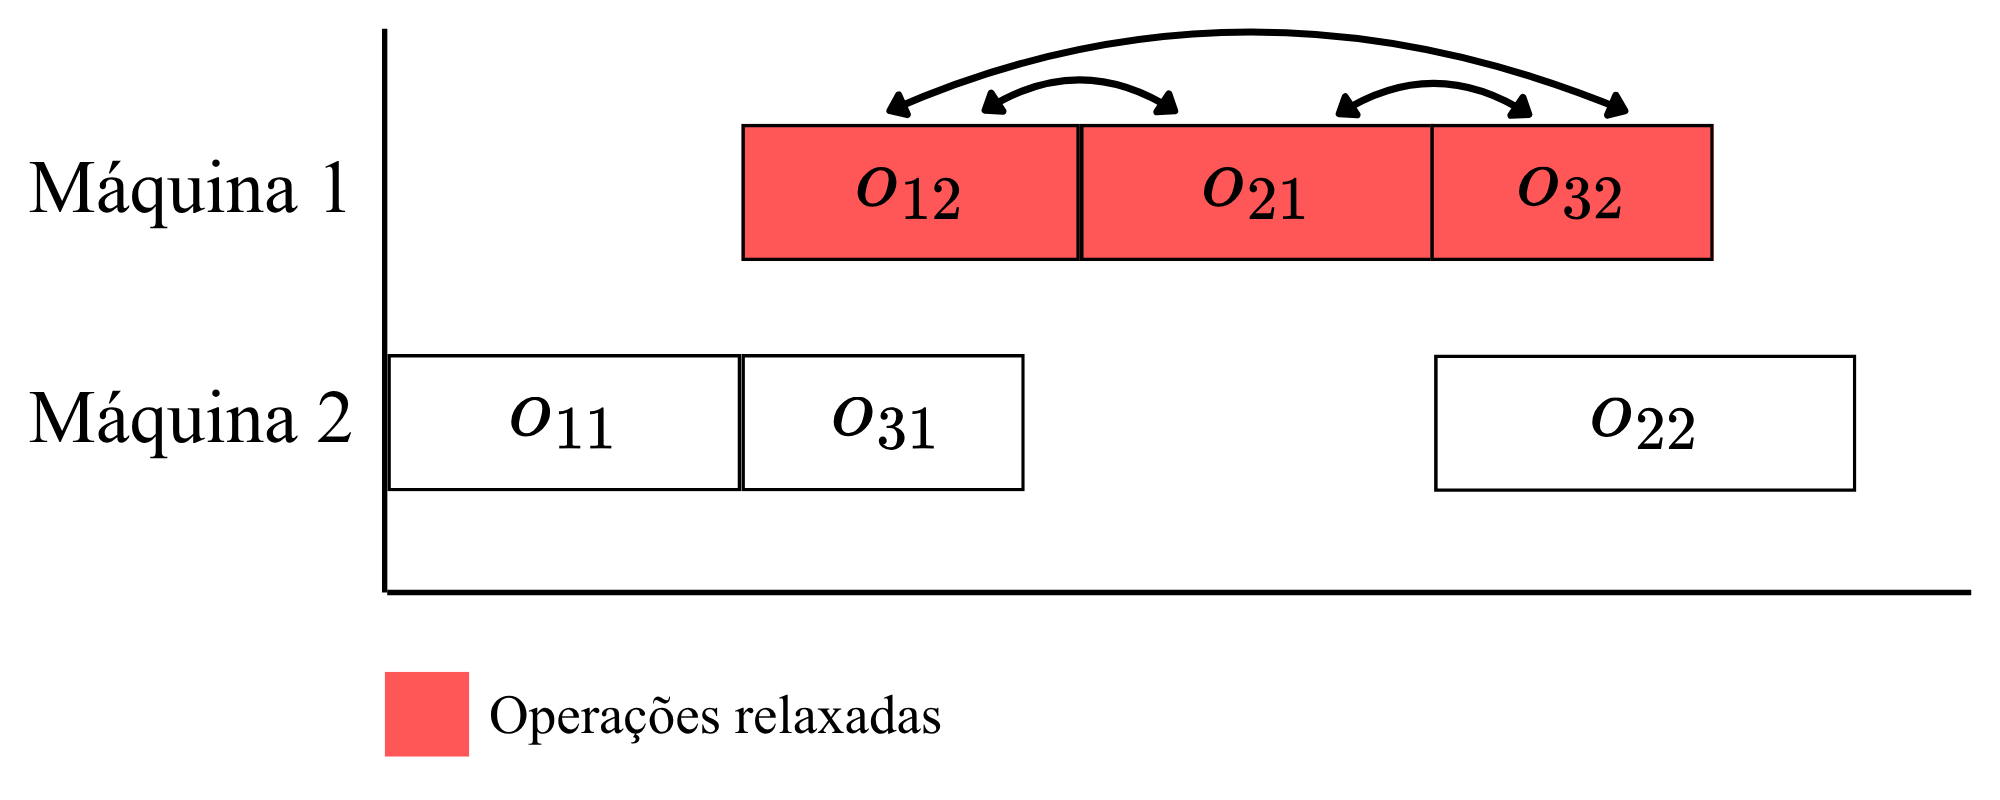
\includegraphics[width=\textwidth]{img/relax_a.png}
         \caption{Agendamento com subconjunto das operações relaxadas pela vizinhança.}
         \label{img:exemplo_relax_a}
     \end{subfigure}
     \hfill
     \begin{subfigure}[b]{0.45\textwidth}
         \centering
         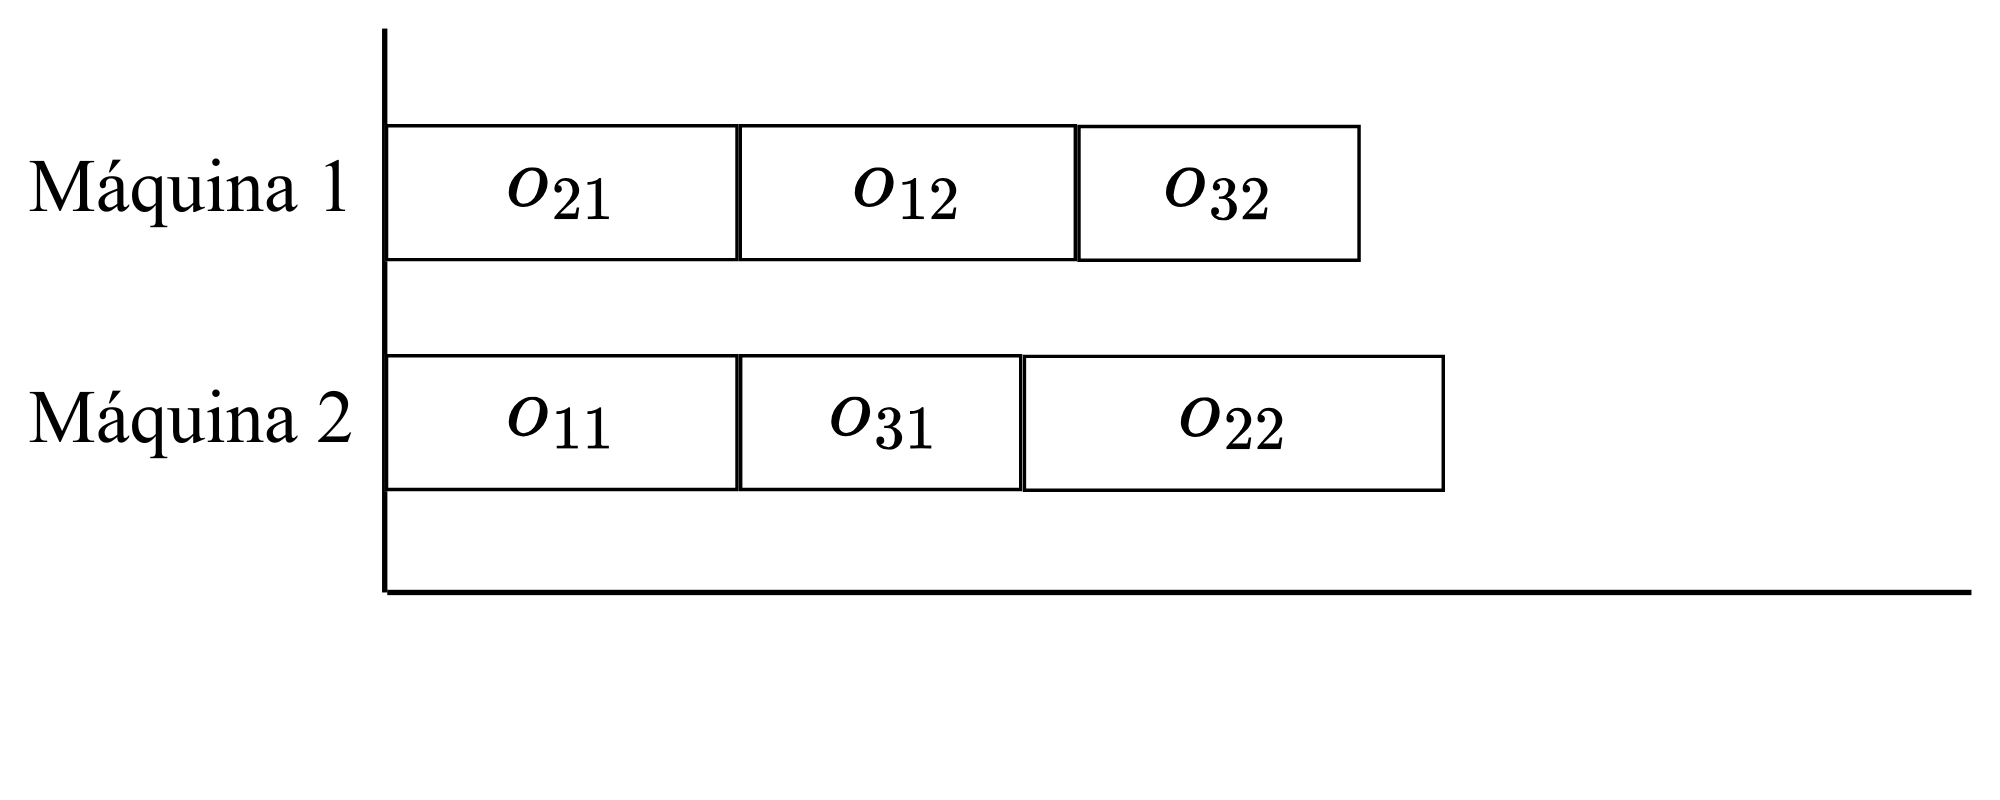
\includegraphics[width=\textwidth]{img/relax_b.png}
         \caption{Agendamento após a reordenação das operações relaxadas.}
         \label{img:exemplo_relax_b}
     \end{subfigure}
     \caption*{Fonte: adaptado de \cite{ahmadian2021meta}}
\end{figure}

A Figura \ref{img:exemplo_relax} ilustra o processo de otimização realizado por este método. No exemplo da Figura \subref{img:exemplo_relax_a}, o algoritmo relaxa a ordem de três operações, permitindo que o solver CPLEX explore qualquer permutação entre elas. Nesse caso, como representado na figura \subref{img:exemplo_relax_b}, as operações são reorganizadas e, por conta disso, todas as operações de ambas as máquinas são adiantadas. 

O projeto divide as demais vizinhanças implementadas em dois grupos: troca e remoção-inserção. As vizinhanças de troca realizam a troca de posição entre duas operações. Já as vizinhanças de remoção-inserção removem uma operação da sua posição e inserem em outra posição da sequência. Recapitulando a Seção \ref{sect:grafo_disj}, restrições de máquina limitam esses deslocamentos estritamente entre operações processadas na mesma máquina.

\begin{figure}[h!]
     \centering
     \caption{Exemplos dos dois tipos principais de vizinhanças: troca e remoção-inserção.}
     \label{fig:exemplos_swap_insert}
     \begin{subfigure}[b]{0.48\textwidth}
         \centering
         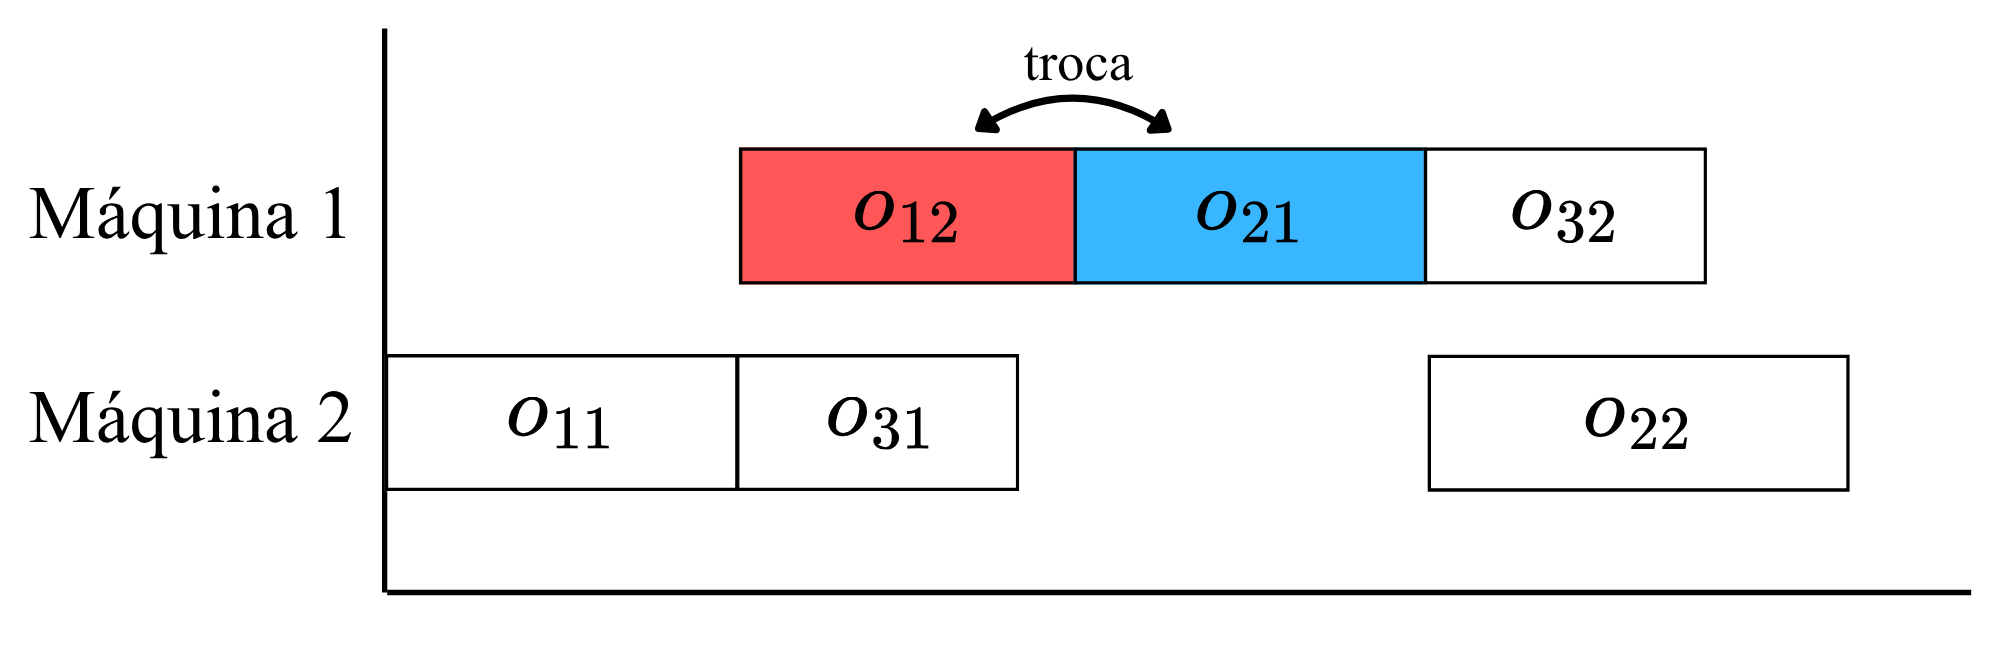
\includegraphics[width=\textwidth]{img/swap_insert_a.png}
         \caption{Agendamento antes de acontecer troca entre $o_{12}$ e $o_{21}$}
         \label{img:exemplos_swap_insert_a}
     \end{subfigure}
     \hfill
     \begin{subfigure}[b]{0.48\textwidth}
         \centering
         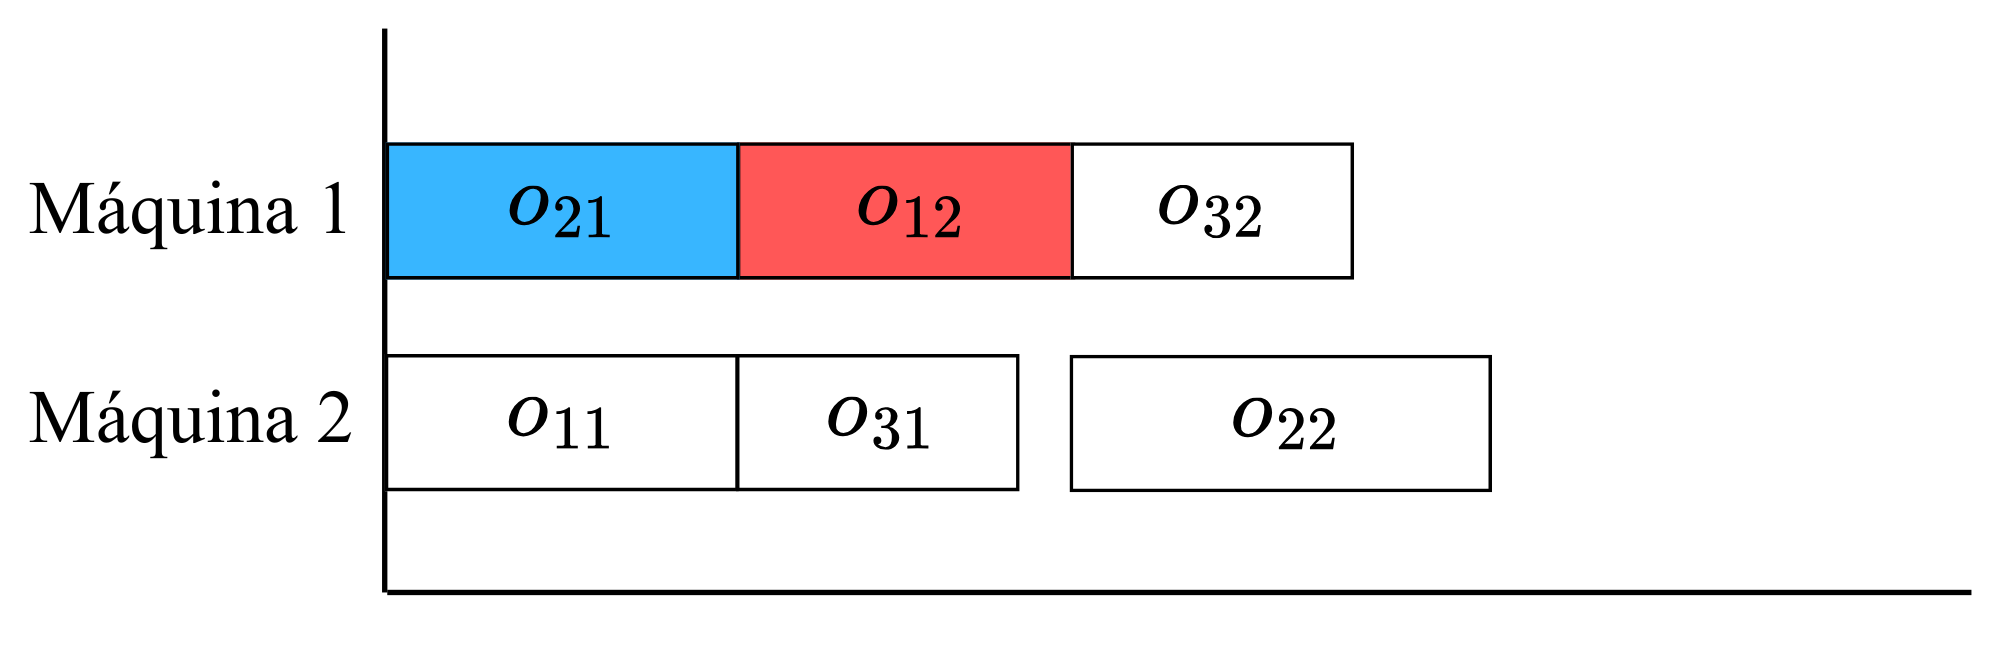
\includegraphics[width=\textwidth]{img/swap_insert_b.png}
         \caption{Agendamento após a troca entre $o_{12}$ e $o_{21}$.}
         \label{img:exemplos_swap_insert_b}
     \end{subfigure}
     
     \vspace{0.5em} % Espaçamento entre as linhas de figuras

     \begin{subfigure}[b]{0.48\textwidth}
         \centering
         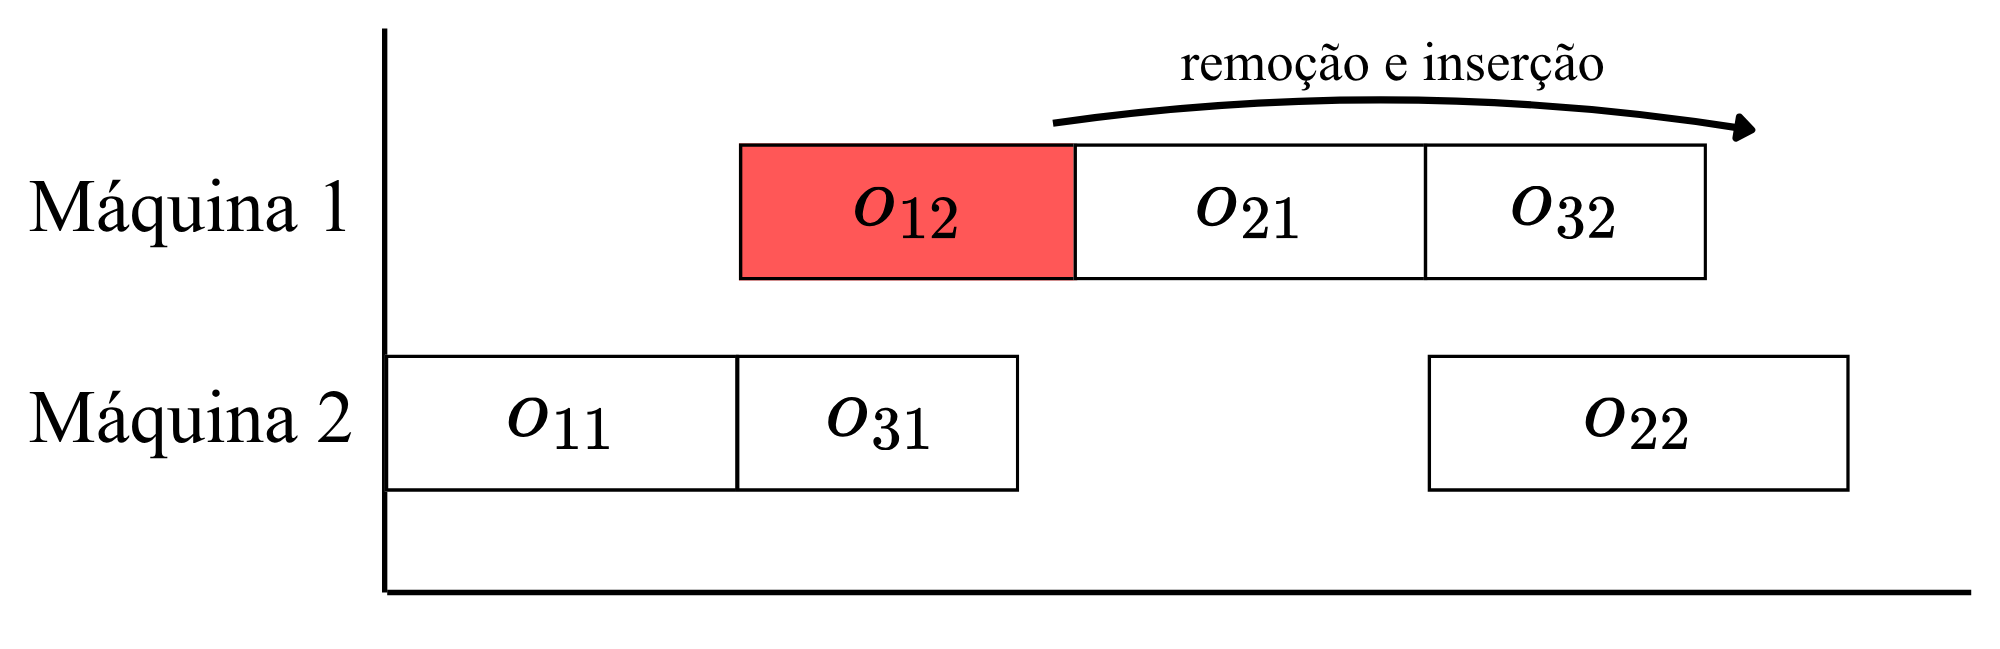
\includegraphics[width=\textwidth]{img/swap_insert_c.png}
         \caption{Agendamento antes de acontecer remoção e inserção de $o_{12}$.}
         \label{img:exemplos_swap_insert_c}
     \end{subfigure}
     \hfill
     \begin{subfigure}[b]{0.48\textwidth}
         \centering
         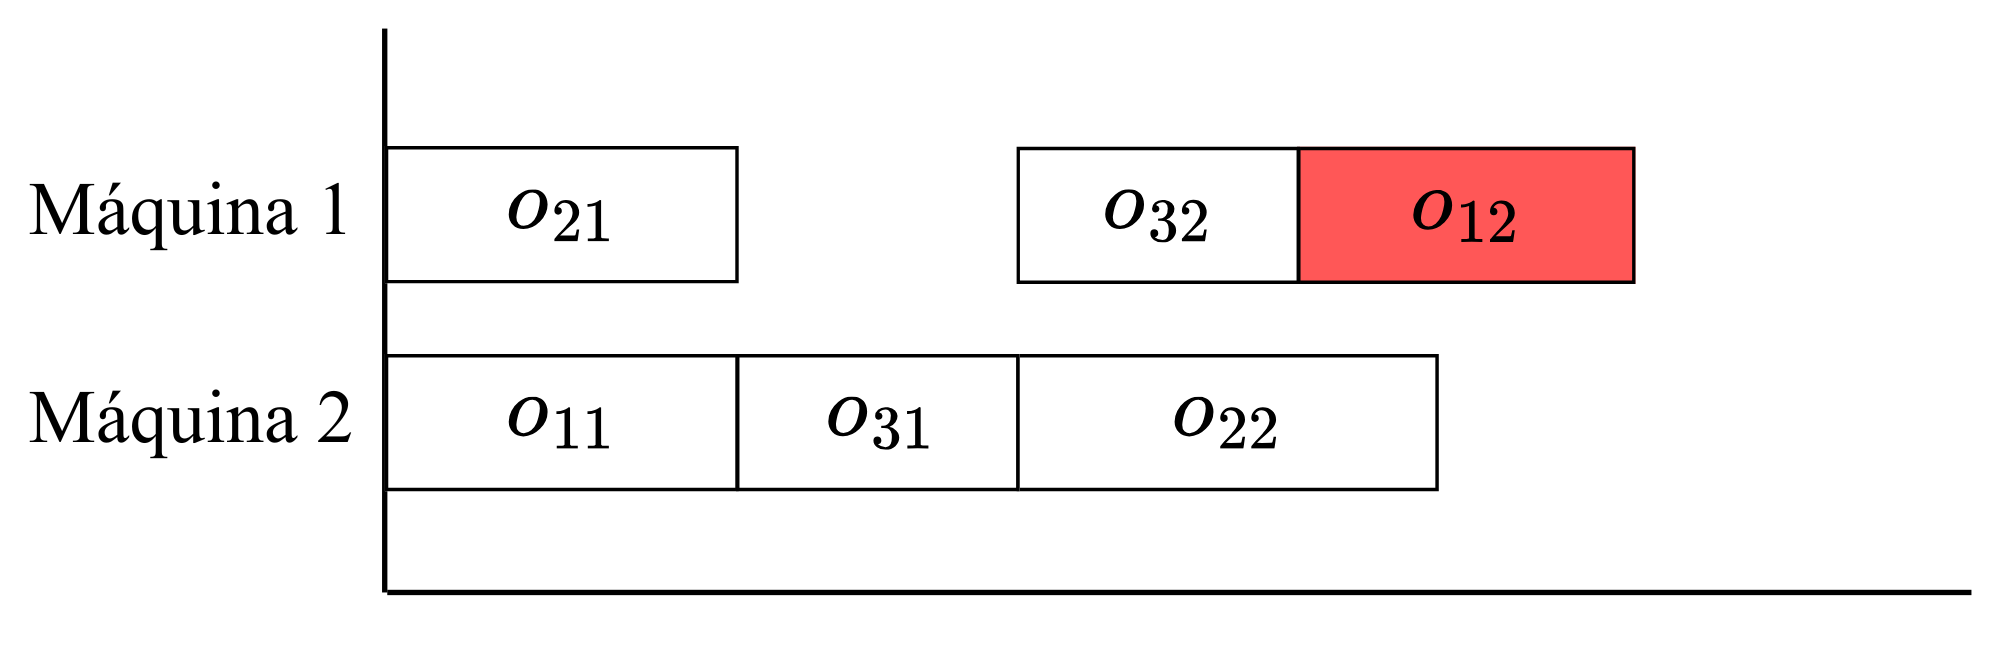
\includegraphics[width=\textwidth]{img/swap_insert_d.png}
         \caption{Agendamento após remoção-inserção com $o_{12}$ no final de uma máquina.}
         \label{img:exemplos_swap_insert_d}
     \end{subfigure}
     \caption*{Fonte: os autores.}
\end{figure}

A Figura \ref{fig:exemplos_swap_insert} apresenta exemplos práticos de ambos os tipos de movimentos. As figuras \subref{img:exemplos_swap_insert_a} e \subref{img:exemplos_swap_insert_b} demonstram a execução de uma troca no agendamento. Já as figuras \subref{img:exemplos_swap_insert_c} e \subref{img:exemplos_swap_insert_d} demonstram a execução de uma remoção de uma operação e inserção em outra posição do agendamento.

Primeiramente, temos as vizinhanças aleatórias utilizadas no trabalho de \cite{ahmadian2021meta}. Uma delas seleciona duas operações aleatoriamente e realiza a troca de posição entre as duas operações, e a outra remove uma operação aleatória e a insere em outra posição aleatória. Chamaremos a primeira de \texttt{troca\_al} e a segunda de \texttt{insere\_al}.

A fundamentação das próximas vizinhanças exige a formalização de definições preliminares. Definimos operações adjacentes entre si como aquelas que não possuem nenhum tempo ocioso entre elas. Dada uma operação $o$, a antecessora e a sucessora de tarefa de $o$ são, respectivamente, as operações que ocorrem antes e depois da operação $o$ dentro da ordem da tarefa de $o$. De forma similar, em uma sequência definida, a antecessora e a sucessora de máquina de $o$ são, respectivamente, as operações que são processadas antes e depois de $o$ na mesma máquina. A notação estabelece $JA(o)$ e $JS(o)$ como a antecessora e sucessora de tarefa, respectivamente, da operação $o$, que também são adjacentes a $o$. Da mesma forma, definimos $MA(o)$ e $MS(o)$, respectivamente, como a antecessora e sucessora de máquina da operação $o$ que também são adjacentes a $o$. Por fim, ao nos referirmos a um bloco de operações, considere um conjunto de operações adjacentes em uma mesma máquina.

A próxima vizinhança possui uma estrutura simplificada. Este componente provém do trabalho de \cite{dos2010combination} e realiza a troca de posição entre uma operação e sua sucessora de máquina, sem nenhum tipo de filtro. Partindo de qualquer solução, essa vizinhança gera sempre um número fixo de vizinhos e contém todas as outras vizinhanças que realizam trocas entre operações adjacentes com algum tipo de filtro. A nomenclatura \texttt{troca\_adj} identifica esta vizinhança.

O trabalho de \cite{wang2014variable} fundamenta outras duas vizinhanças que são baseadas nas penalidades das operações. A vizinhança de troca baseia-se no seguinte lema. Se uma operação $o$ está atrasada, $MA(o)$ não existe e $JA(o)$ existe, então $JA(o)$ também está atrasada. E, no caso inverso, se uma operação $o$ está adiantada, $MS(o)$ não existe e $JS(o)$ existe, então $JS(o)$ também está atrasada. Nesse sentido, a partir de uma operação $o$ adiantada (ou atrasada), o algoritmo percorre o agendamento seguindo as operações $JS(o)$ (ou $JA(o)$) até encontrar uma operação que possua uma $MS(o)$ (ou $MA(o)$) ou encontrar uma operação que seja a última (ou a primeira) operação da máquina ou da tarefa. A nomenclatura \texttt{troca\_penal} identifica esta vizinhança.

\begin{figure}[h!]
     \centering
     \caption{Exemplo de modificação de soluções pela vizinhança troca\_penal.}
     \label{img:exemplo_swap_penal}
     \begin{subfigure}[b]{0.45\textwidth}
         \centering
         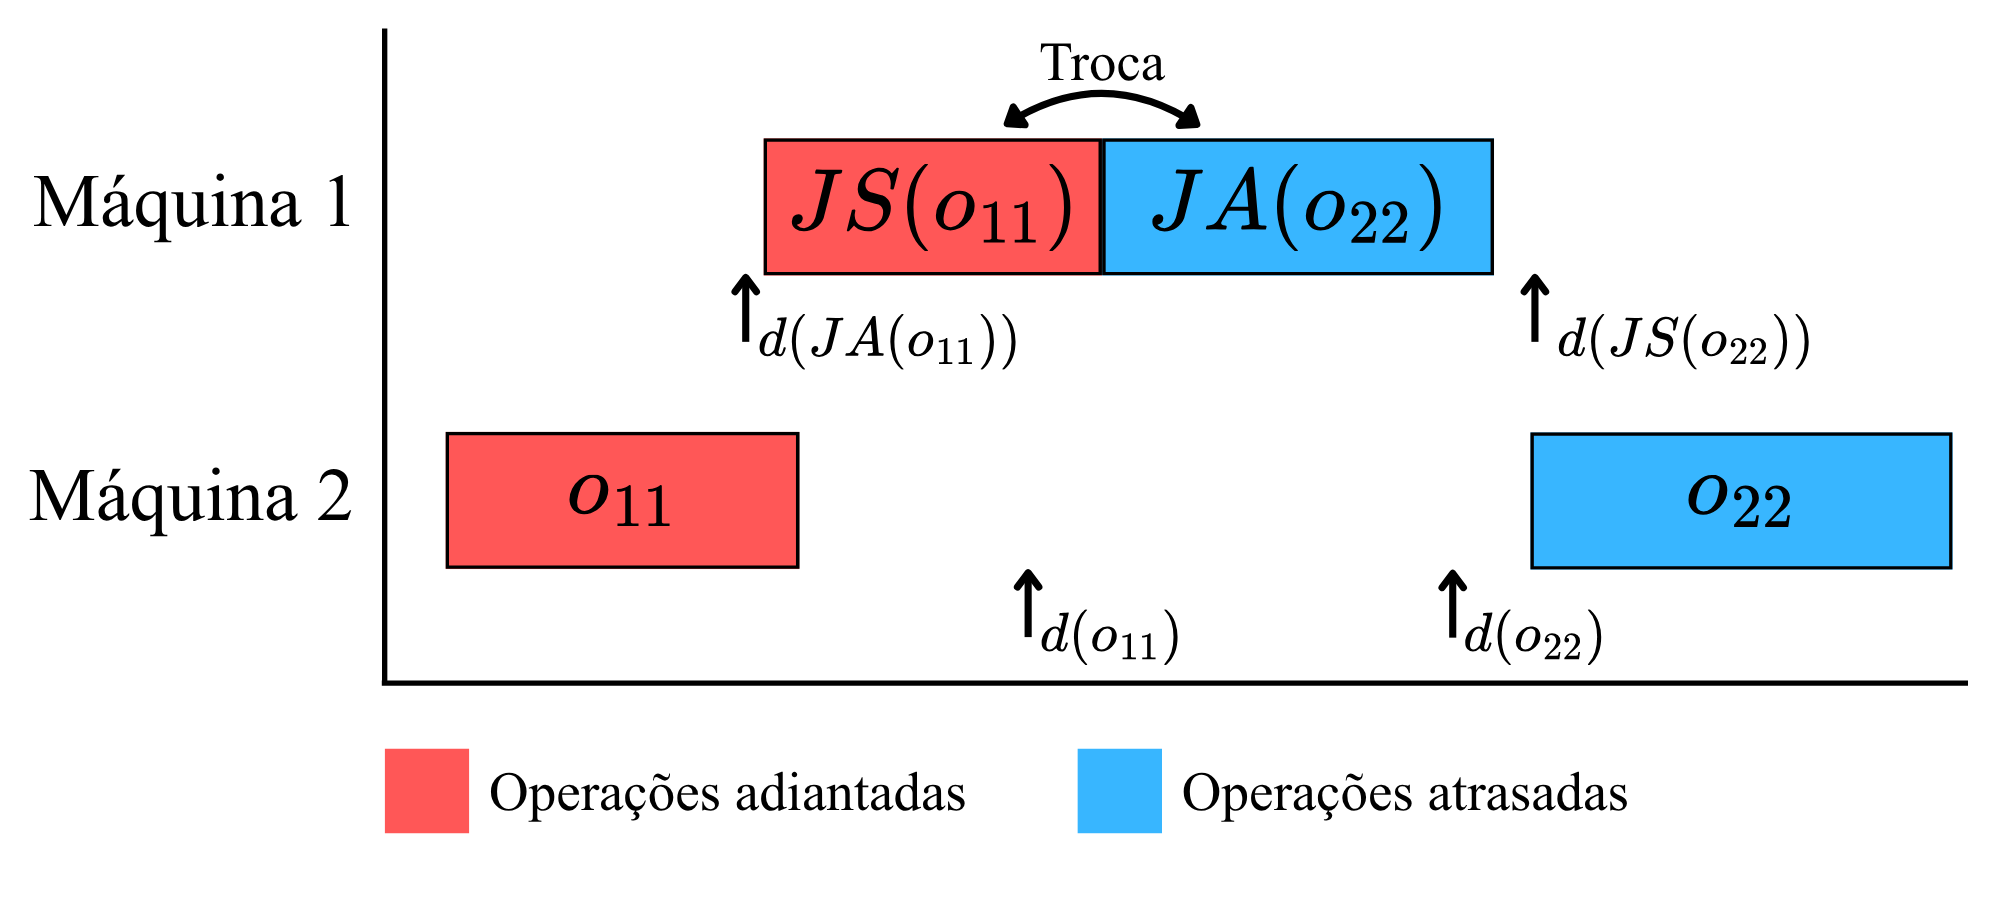
\includegraphics[width=\textwidth]{img/swap_penal_a.png}
         \caption{Agendamento com operações atrasadas e adiantadas com possível modificação pela vizinhança troca\_penal.}
         \label{img:exemplo_swap_penal_a}
     \end{subfigure}
     \hfill
     \begin{subfigure}[b]{0.45\textwidth}
         \centering
         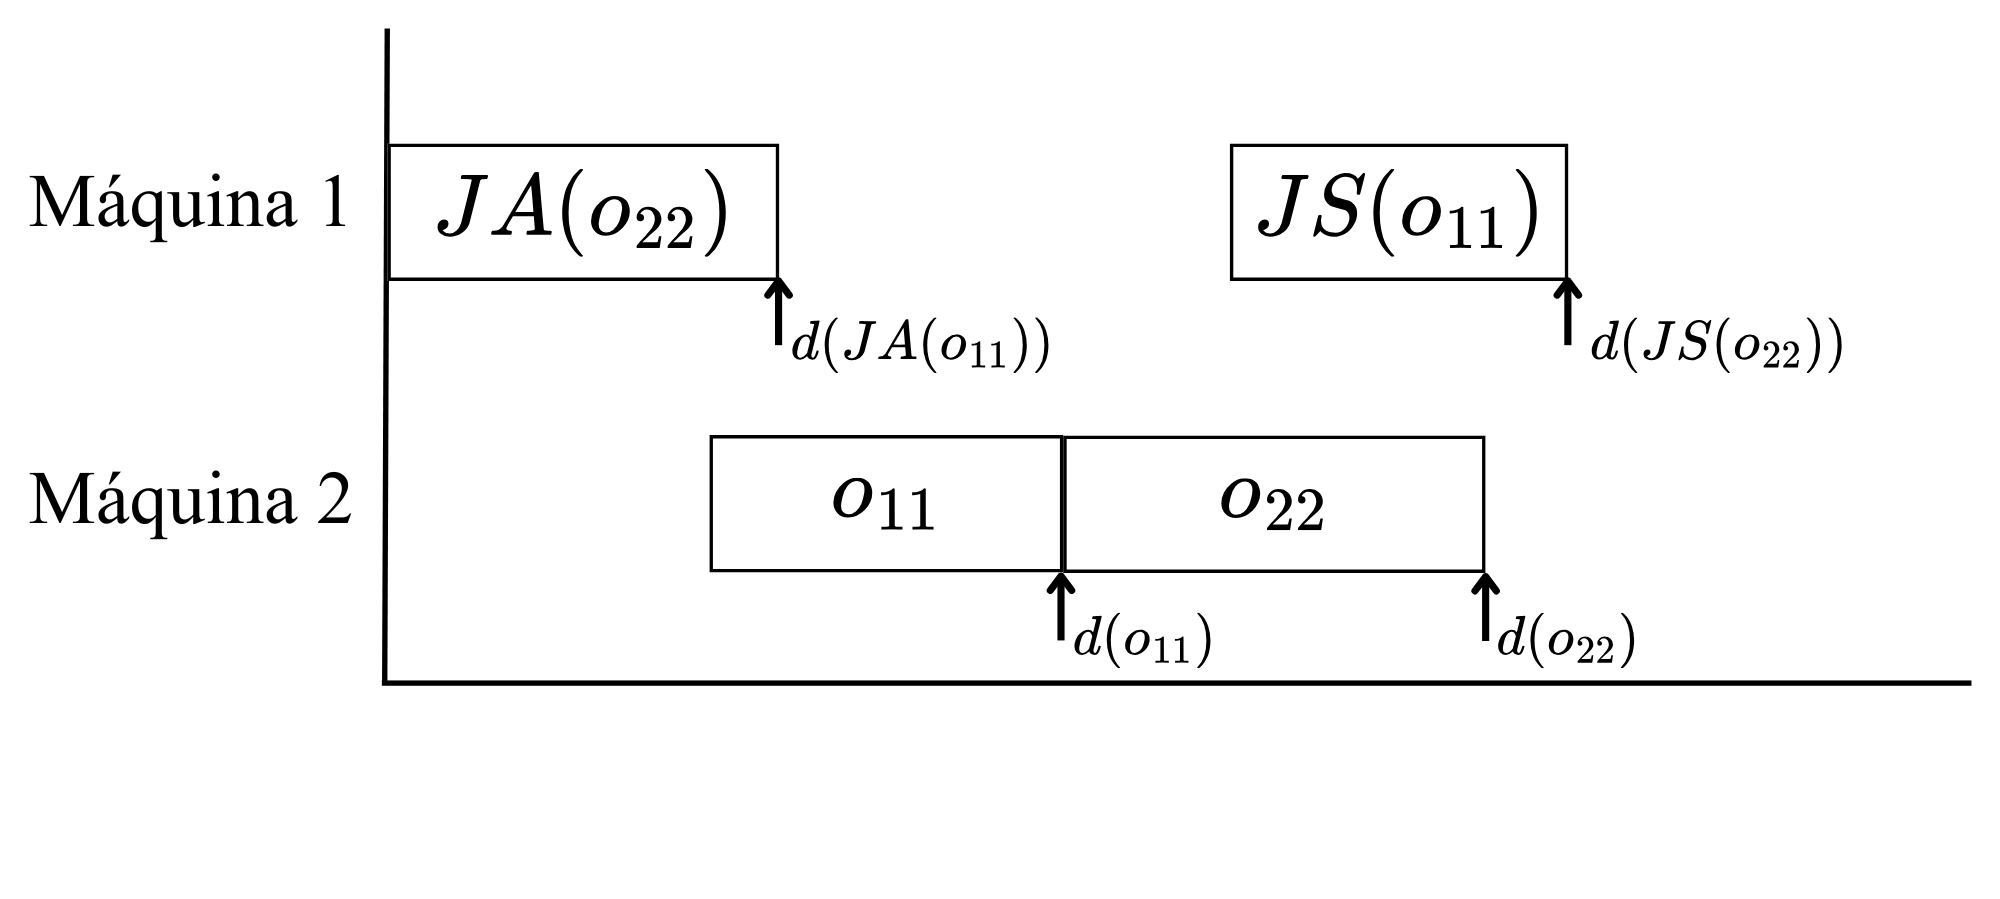
\includegraphics[width=\textwidth]{img/swap_penal_b.png}
         \caption{Agendamento após a modificação da vizinhança troca\_penal com todas as operações entregues nos seus prazo de entrega.}
         \label{img:exemplo_swap_penal_b}
     \end{subfigure} 
     \caption*{Fonte: Adaptado de \cite{wang2014variable}}
\end{figure}

Por exemplo, na Figura \ref{img:exemplo_swap_penal} podemos observar um exemplo de aplicação desta vizinhança. A partir da operação adiantada $o_{11}$, ao seguir a sucessora $JS(o_{11})$, o procedimento localiza uma troca capaz de zerar as penalidades de todas as operações envolvidas. De forma semelhante, a partir da operação atrasada $o_{22}$, seguindo a antecessora $JA(o_{22})$, o algoritmo encontraria a mesma troca. 

No caso da vizinhança de remoção-inserção baseada nas penalidades, se uma operação está adiantada, a vizinhança remove a operação e tenta inseri-la ao final do bloco correspondente. Por outro lado, se uma operação está atrasada, a vizinhança a remove e tenta inseri-la no início do bloco. Todo o procedimento condiciona a inserção ao agendamento atual para preservar a localidade do movimento. Para uma operação adiantada $o$ que seria inserida ao final do bloco, se o tempo de término do bloco for maior que o tempo de início da sucessora de tarefa de $o$, então $o$ é inserida após a primeira operação do bloco que possui tempo de término menor que o tempo de início de sua sucessora de tarefa. Da mesma maneira, para uma operação atrasada que seria inserida no início do bloco, se o tempo de início do bloco for menor que o tempo de término da antecessora de tarefa de $o$, então $o$ será inserida antes da primeira operação do bloco que possuir tempo de início maior que o tempo de término da sua antecessora. A nomenclatura \texttt{insere\_penal} identifica esta vizinhança.

A Figura \ref{fig:exemplos_insert_penal_earl} ilustra como essa modificação acontece, juntamente com o mecanismo de controle do impacto das modificações. Nessa figura, a operação $u$ está adiantada e a vizinhança tentaria inseri-la no fim do seu bloco, isto é, após a operação $w$. No primeiro cenário, nas figuras \subref{img:exemplos_insert_penal_earl_a} e \subref{img:exemplos_insert_penal_earl_b}, $JS(u)$ tem um tempo de início maior que o término do bloco, ou seja, inserir $u$ no fim do bloco não afetaria o tempo de inicio de sua sucessora, então, o movimento acontece. Já no segundo cenário, nas figuras \subref{img:exemplos_insert_penal_earl_c} e \subref{img:exemplos_insert_penal_earl_d}, inserir $u$ no fim do bloco não é possível sem atrasar sua sucessora. Por isso, a inserção é realizada antes da operação $w$, mantendo a posição anterior de $JS(u)$. Quando nossa operação alvo está atrasada, esse processo acontece de forma similar, porém observando os critérios descritos no parágrafo anterior.

\begin{figure}[h!]
     \centering
     \caption{Exemplos das modificações da vizinhança insere\_penal para um operação adiantada.}
     \label{fig:exemplos_insert_penal_earl}
     \begin{subfigure}[b]{0.48\textwidth}
         \centering
         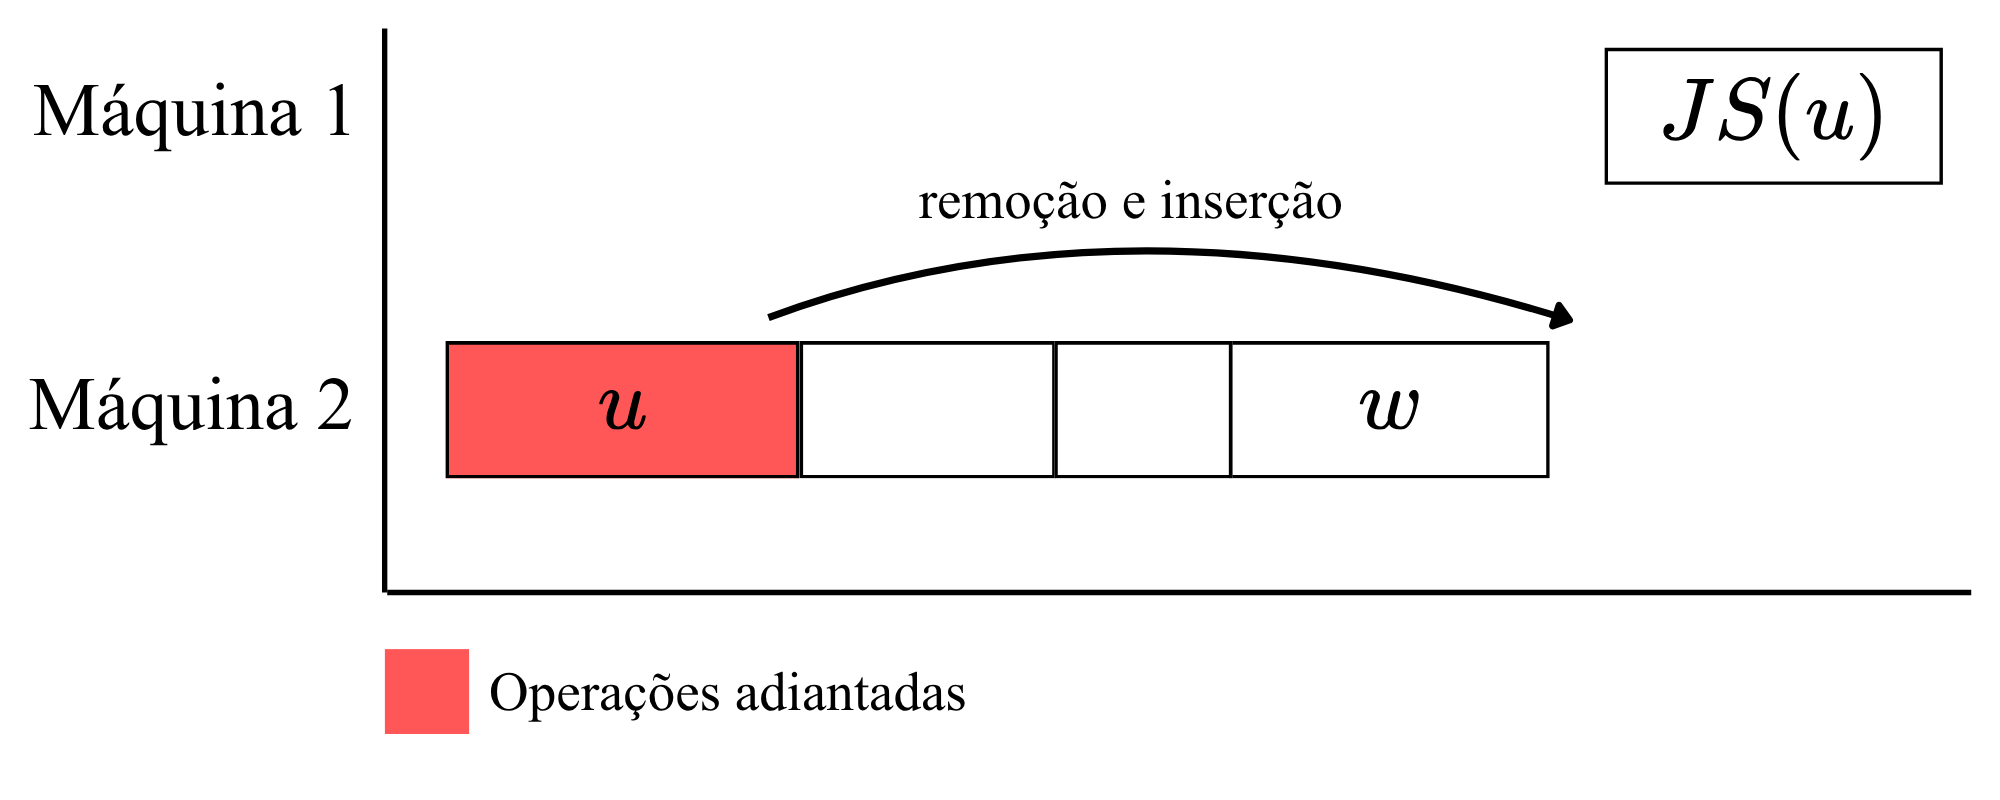
\includegraphics[width=\textwidth]{img/insert_penal_earl_a.png}
         \caption{Agendamento com operação $u$ adiantada e tempo de início de $JS(u)$ maior que tempo de término do bloco.}
         \label{img:exemplos_insert_penal_earl_a}
     \end{subfigure}
     \hfill
     \begin{subfigure}[b]{0.48\textwidth}
         \centering
         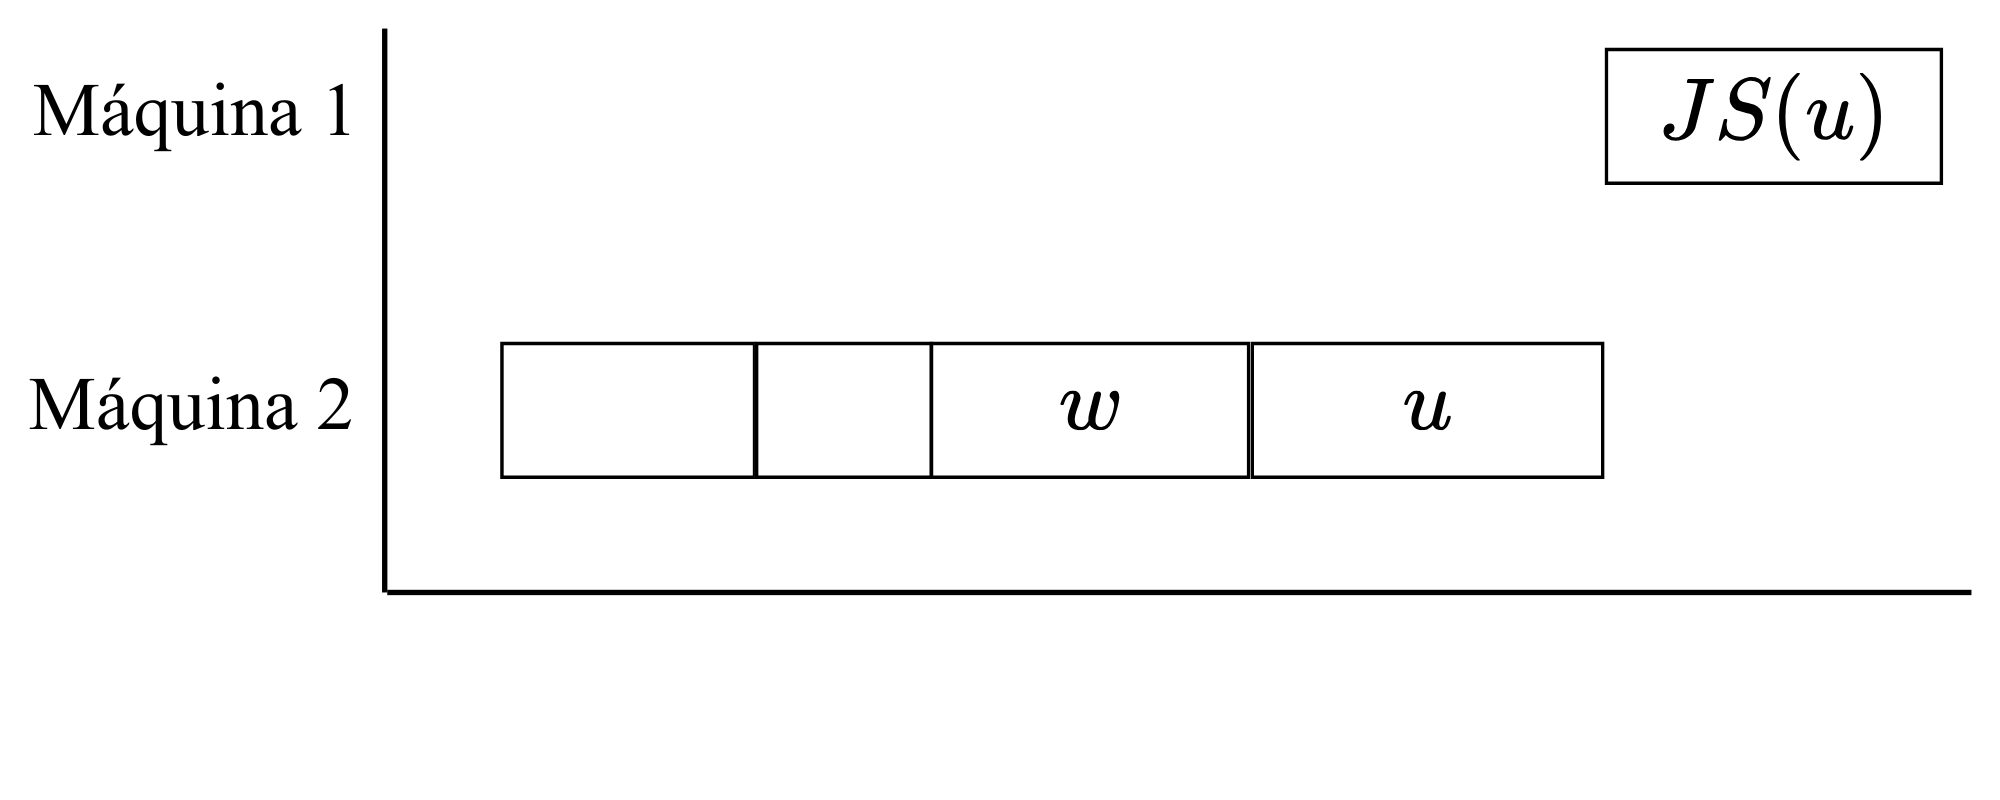
\includegraphics[width=\textwidth]{img/insert_penal_earl_b.png}
         \caption{Agendamento após inserção de $u$ no fim do bloco tendo sua penalidade de adiantamento reduzida.}
         \label{img:exemplos_insert_penal_earl_b}
     \end{subfigure}
     
     \vspace{0.3em} % Espaçamento entre as linhas de figuras

     \begin{subfigure}[b]{0.48\textwidth}
         \centering
         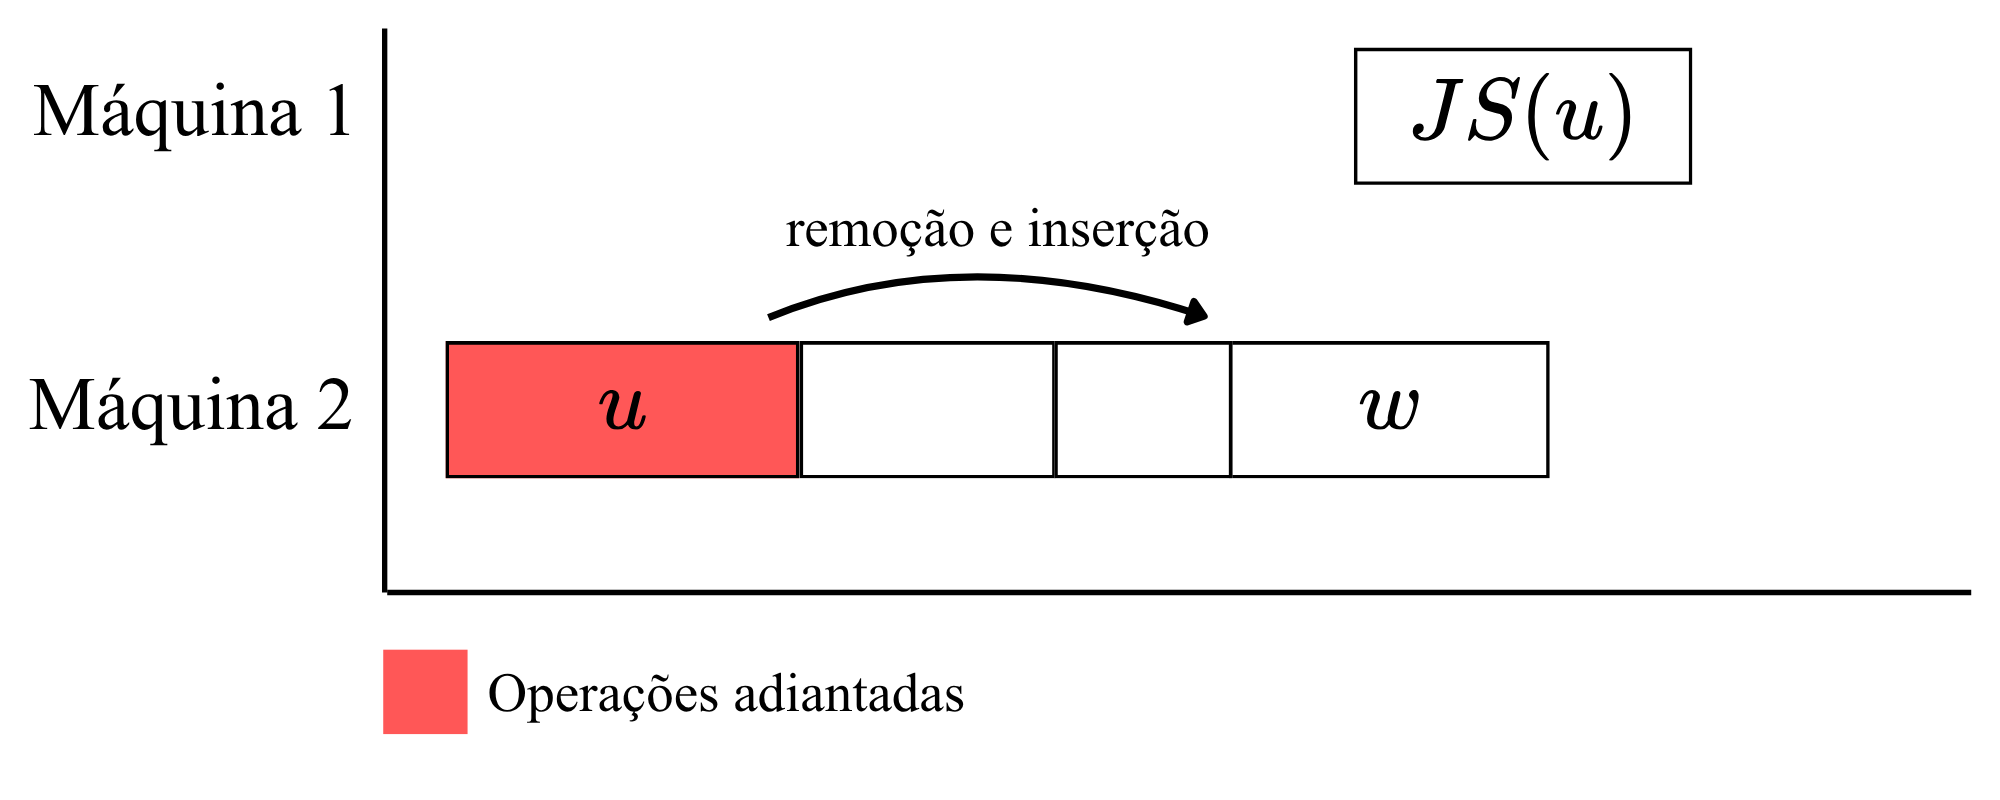
\includegraphics[width=\textwidth]{img/insert_penal_earl_c.png}
         \caption{Agendamento com operação $u$ adiantada e tempo de início de $JS(u)$ menor que tempo de término do bloco.}
         \label{img:exemplos_insert_penal_earl_c}
     \end{subfigure}
     \hfill
     \begin{subfigure}[b]{0.48\textwidth}
         \centering
         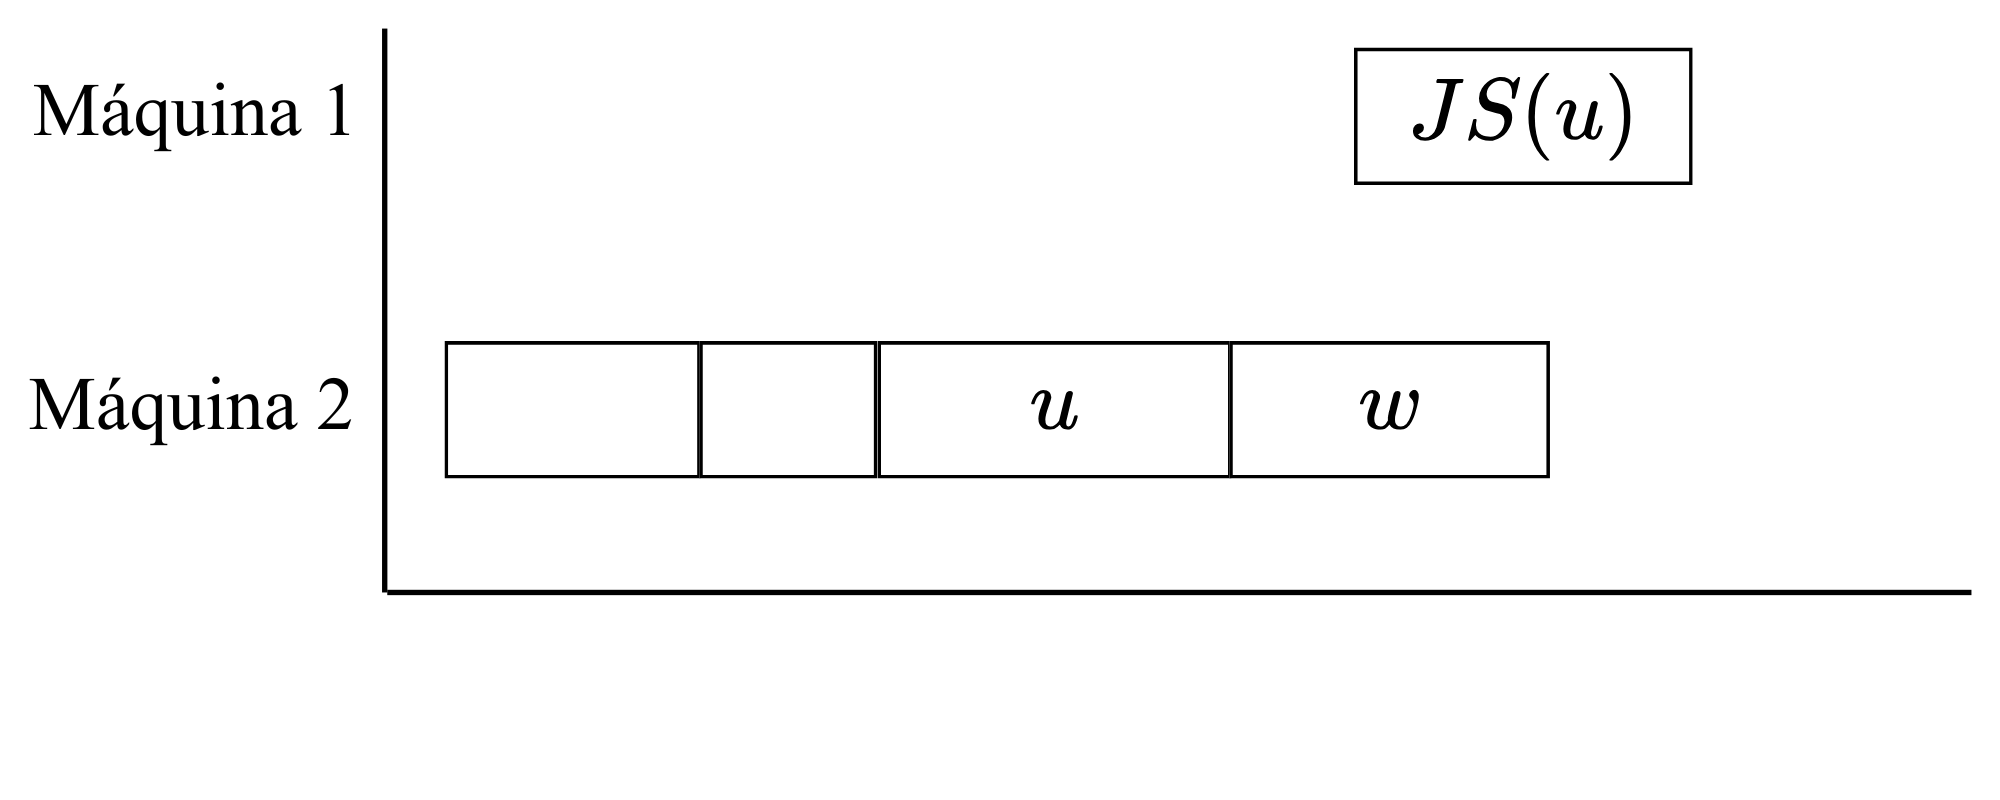
\includegraphics[width=\textwidth]{img/insert_penal_earl_d.png}
         \caption{Agendamento após inserção de $u$ no meio do bloco ainda tendo sua penalidade de adiantamento reduzida.}
         \label{img:exemplos_insert_penal_earl_d}
     \end{subfigure}
     \caption*{Fonte: adaptado de \cite{wang2014variable}.}
\end{figure}

Por fim, este trabalho propõe uma vizinhança original ao \ac{JITJSS}, fundamentada na estrutura N5 de \cite{nowicki1996fast} para o problema \ac{JSS}, mas adaptada para a redução de penalidades por atraso. Os autores propõem uma vizinhança que explora o conceito explicado na Seção \ref{sect:grafo_disj} de que apenas alterações no caminho crítico de um agendamento alteram seu \textit{makespan}. Nesse sentido, a vizinhança consiste em realizar a troca de posição entre as duas primeiras e as duas últimas operações de cada um dos blocos críticos do agendamento, isto é, blocos de operações que estão contidos no caminho crítico. Perceba que a ideia da otimização do \textit{makespan} é adiantar o tempo de início da última operação do caminho crítico.

% \begin{figure}[h!] 
%     \centering 
%     \caption{Exemplo da vizinhança RELAX}
%     \label{img:exemplo_viz_insert_penal_tard}
%     \includegraphics[width=0.9\linewidth]{img/insert_penal_tard.png}
%     \caption*{\small \textbf{Fonte:} Os Autores.}
% \end{figure}

Dessa forma, a vizinhança proposta aplica o conceito de caminho crítico individualmente para cada uma das operações atrasadas do agendamento. Para isso, dada uma operação $o$ atrasada, o algoritmo compõe o caminho crítico ao percorrer as antecessoras de $o$ de forma iterativa. A cada iteração, a nova operação a ser adicionada no caminho crítico será a operação com o maior tempo de término entre $JA(o)$ e $MA(o)$, isto é, a operação que impede a operação atual de ser adiantada. A construção do caminho crítico de $o$ termina após encontrar uma operação que não possui nem $JA$ nem $MA$. A posse desse caminho crítico permite ao algoritmo gerar vizinhos da solução original por meio da estrutura N5. A nomenclatura \texttt{troca\_crit} identifica esta vizinhança.

\begin{figure}[h!] 
    \centering 
    \caption{Exemplo de modificações vizinhas geradas pela vizinhança troca\_crit.}
    \label{img:exemplo_viz_critical}
    
\includegraphics[width=0.75\linewidth]{img/oper_crit.png}
    \caption*{\small \textbf{Fonte:} Os Autores.}
\end{figure}

A Figura \ref{img:exemplo_viz_critical} apresenta um cenário no qual a operação $o_{12}$ está atrasada, isto é, reduzir seu tempo de início pode contribuir para a redução das penalidades. A aplicação da vizinhança \texttt{troca\_crit} exige a identificação do caminho crítico específico da operação em questão. A execução do processo descrito no parágrafo anterior resulta na identificação das operações destacadas em vermelho como o caminho crítico de $o_{12}$. Essas operações representam o caminho de dependência da operação $o_{12}$, e apenas a modificação delas é capaz de reduzir o tempo de início de $o_{12}$. A partir disso, esse caminho crítico gera três vizinhos a partir das trocas das operações $o_{11}$ com $o_{31}$, $o_{32}$ com $o_{21}$ e $o_{21}$ com $o_{12}$. Trocas estas que correspondem aos pares de operações nas extremidades de cada bloco crítico.

\subsection{Métodos de busca}

A exploração das vizinhanças a partir de uma solução inicial requer o emprego de métodos de busca heurística. Para isso, o projeto contempla três opções de métodos de busca: uma busca local simples conforme explicada na Seção \ref{sect:meta}, a busca tabu e a busca local iterada.

A busca tabu segue o que foi definido na seção \ref{sect:meta}, mas com a adição de mecanismos que melhoram a intensificação e a exploração do processo de busca. Primeiramente, precisamos definir como a lista tabu armazenará os movimentos que devem ser proibidos enquanto forem tabu. A estrutura de memória registra exclusivamente as arestas do grafo disjuntivo desfeitas pelas modificações na solução. Essa abordagem garante a representação universal de qualquer movimento, uma vez que o grafo disjuntivo sustenta todas as soluções do problema. O detalhe é que cada um dos tipos de modificações é armazenado de forma ligeiramente diferente.

Nas vizinhanças de troca entre duas operações, o algoritmo classifica as arestas de entrada das operações envolvidas como tabu. Por exemplo, se uma máquina possui a seguinte ordem de operações $o1 \xrightarrow{} o2 \xrightarrow{} o3 \xrightarrow{} o4 \xrightarrow{} o5$, então as arestas $\{(o1,o2),(o2,o3),(o3,o4), (o4,o5)\}$ existem no grafo disjuntivo. Se uma vizinhança realiza a troca de posição entre as operações $o2$ e $o4$, então as arestas $(o1,o2)$ e $(o3,o4)$ se tornam tabu. Isso impede, neste exemplo, o retorno das operações $o2$ e $o4$ às posições sucessoras de $o1$ e $o2$ durante a vigência do \textit{tenure}. 

Nas vizinhanças de remoção-inserção, apenas a aresta de entrada da operação removida é adicionada como tabu. No mesmo exemplo do parágrafo anterior, se a operação $o2$ for removida e inserida após $o3$, então a aresta $(o1,o2)$ se torna tabu. Com isso, $o2$ é impedida de retornar como sucessora de $o1$ nas próximas iterações.

A verificação da lista tabu acontece durante a exploração da vizinhança pela busca tabu. Durante esse processo, dada uma lista de opções de modificações geradas por uma vizinhança, o procedimento de busca avalia as modificações geradas e seleciona o movimento conforma a seguinte hierarquia de prioridade:

\begin{enumerate}
    \item A melhor modificação, seja ela tabu ou não, que seja menor que a melhor solução encontrada até o momento. Este item aplica o critério de aspiração na exploração da vizinhança.
    \item A melhor modificação que não seja tabu.
    \item A modificação mais antiga da lista tabu.
\end{enumerate}

Todo movimento escolhido é adicionado à lista tabu de acordo com seu tipo, conforme descrito anteriormente. Esse movimento continuará tabu durante um número de iterações determinado pelo \textit{tabu tenure}. A meta-heurística incrementa a contagem de tempo da lista a cada nova inserção. Além disso, caso o algoritmo selecione a modificação tabu mais antiga durante a exploração, o sistema adianta o relógio da lista até o instante em que tal movimento perderia a condição de tabu, removendo simultaneamente da lista elementos mais antigos. Por exemplo, se uma lista tabu possui \textit{tabu tenure} igual a 20 e $5$ elementos que foram adicionados há $2$, $7$, $12$, $14$ e $16$ iterações. Se a modificação com idade $12$ foi escolhida dentro de alguma vizinhança, as iterações da lista tabu serão avançadas em $8$, fazendo com que os elementos com mais idade que $12$ também saiam da lista tabu, restando dois elementos com idades de $10$ e $15$ iterações.

Além da lista tabu, a implementação integra dois mecanismos baseados no trabalho de \cite{zubaran2016tabu} para otimizar a exploração do espaço de busca: uma lista de soluções elite para intensificação e um detector de ciclos para evitar estagnação. A lista de elites $E$ contém as $L$ melhores soluções encontradas durante a busca. Quando uma nova solução gera melhoria, ela é adicionada a $E$. Caso $E$ esteja em sua capacidade máxima, a solução mais antiga é removida. Além disso, o sistema armazena, para cada entrada em $E$, o estado completo da busca, incluindo a lista de vizinhos que ainda não foram explorados e a configuração atual da lista tabu.

A busca inicia em uma solução inicial $s^*$ e explora as vizinhanças a partir dela por um orçamento de até $I$ iterações. O algoritmo reinicia o orçamento de iterações $I$ sempre que identifica uma melhoria na solução atual. Ao atingir o limite de iterações determinado por $I$, ou ao detectar um ciclo, a busca retoma a exploração a partir da solução elite mais recente, selecionando um de seus vizinhos ainda não explorados. Este movimento de diversificação aplica um fator de redução $F$ sobre o orçamento máximo $I$. Se nenhuma solução elite existir, a busca para.

Por fim, o detector de ciclos mencionado anteriormente consiste no armazenamento de uma lista de valores de soluções passadas. A partir disso, a busca tabu verifica a repetição desses valores objetivos a cada iteração. Caso essa repetição ocorra mais do que um número máximo de vezes, um ciclo é detectado e o processo descrito no parágrafo anterior é executado.

O terceiro método de busca no espaço de projeto consiste na busca local iterada. Como descrita na Seção \ref{sect:meta}, ela é capaz de utilizar internamente tanto a busca local quanto a busca tabu como heurísticas de busca. Ao utilizar a busca local, ela se comporta como uma \ac{ILS} comum, e ao utilizar a busca tabu, ela se comporta como uma busca tabu iterada. A cada iteração da \ac{ILS}, ela realiza uma perturbação na solução base. Nesse sentido, o algoritmo utiliza a estratégia de perturbação proposta por \cite{ahmadian2021meta}. Ela consiste em escolher duas máquinas aleatoriamente e relaxar as restrições de precedência das máquinas em diversas operações. Dessa forma, o procedimento submete o modelo relaxado ao solver CPLEX com um limite de tempo de 1 segundo, permitindo que a ferramenta reorganize as operações e gere uma nova configuração inicial para a próxima busca local. gerando uma nova solução modificada.

Além disso, considerando que o atual estado da arte para o \ac{JITJSS} é um \ac{VNS}, a estrutura da \ac{ILS} admite a integração de uma coleção de vizinhanças, operando de forma análoga ao \ac{VNS}. Nesse âmbito, a meta-heurística respeita a ordem de entrada das vizinhanças durante a exploração do espaço de busca. A cada iteração sem melhora, a busca realiza uma perturbação e tenta utilizar a próxima vizinhança da lista em busca de melhorias na solução. Caso aconteça alguma melhoria na solução ou caso a coleção de vizinhanças chegue ao fim sem nenhuma melhora, a busca reinicia o ciclo das vizinhanças. Ademais, o espaço de projeto permite a alternância entre os critério de melhor melhora ou primeira melhora para cada vizinhança integrante da lista.

Ambos os métodos, busca local e busca tabu, são capazes de executar a exploração das vizinhanças sob os critérios de melhor melhora ou primeira melhora, com a única exceção sendo a vizinhança \texttt{relax}. No caso da exploração por primeira melhora, os movimentos candidatos são todos gerados e embaralhados aleatoriamente com o objetivo de remover algum viés causado pela ordem da geração dos vizinhos. Além disso, uma limitação importante é que a busca tabu não é capaz de utilizar a vizinhança \texttt{relax}. Visto que o solver realiza a sua própria exploração da vizinhança, a busca tabu perde visibilidade sobre as transições individuais de estados e, por isso, não consegue montar suas estruturas de intensificação e diversificação.

\subsection{Agendadores}

A avaliação da qualidade de uma sequência exige métodos de agendamento precisos, conforme discutido na Seção \ref{sect:grafo_disj}. Nesse sentido, a literatura do \ac{JITJSS} recorre frequentemente à programação inteira para converter sequências em agendamentos (Seção \ref{sect:bibjitjsp}). Por isso, o espaço de projeto contempla esta abordagem por meio da integração com o solver CPLEX. O modelo submetido ao solver fixa a ordem das máquinas e permite ao solver apenas determinar as posições temporais de cada operação.

O projeto integra, adicionalmente, um algoritmo de agendamento utilizado na minimização do \textit{makespan} no problema \ac{JSS}. Esse algoritmo consiste em agendar as operações o mais cedo possível, com complexidade linear. Porém, como discutido na Seção \ref{sect:grafo_disj}, essa forma de agendamento tende a gerar penalidades de adiantamento desnecessárias. Para mitigar esse efeito, o sistema adota a lógica de \cite{ferreira2023}. Após realizar o agendamento da forma descrita, o algoritmo percorre a solução, atrasando operações adiantadas que possuem tempo ocioso subsequente. O algoritmo restringe esse deslocamento a cenários que não impactam operações no prazo ou em atraso, garantindo que o procedimento preserve ou melhore o valor da função objetivo em todos os casos.

\section{Configuração automática} \label{sect:confauto}

Como proposto na metodologia e descrito no referencial teórico, agora que temos o espaço de projeto construído, precisamos formalizá-lo de forma que seja possível parametrizar a geração automática de algoritmos. Para isso, utilizaremos uma gramática livre de contexto.

\subsection{Gramática e parâmetros}

A Figura \ref{img:gramatica_final} contém a gramática que gera todas as combinações algorítmicas que o espaço de projeto admite. Todas as meta-heurísticas precisam de uma solução inicial (\texttt{sol\_ini}), que pode ser o algoritmo de \ac{GT} (\texttt{gt}) ou o algoritmo construtivo comum (\texttt{constr}). Ambas as soluções iniciais precisam de uma regra de despacho (\texttt{regra\_desp}) que pode ser aleatória (\texttt{aleatoria}), a \ac{EDD} (\texttt{edd}) ou a regra ALL+CR+SPT (\texttt{acs}).

\begin{figure}[h!] 
    \centering 
    \caption{Gramática livre de contexto para geração dos algoritmos}
    \label{img:gramatica_final}
    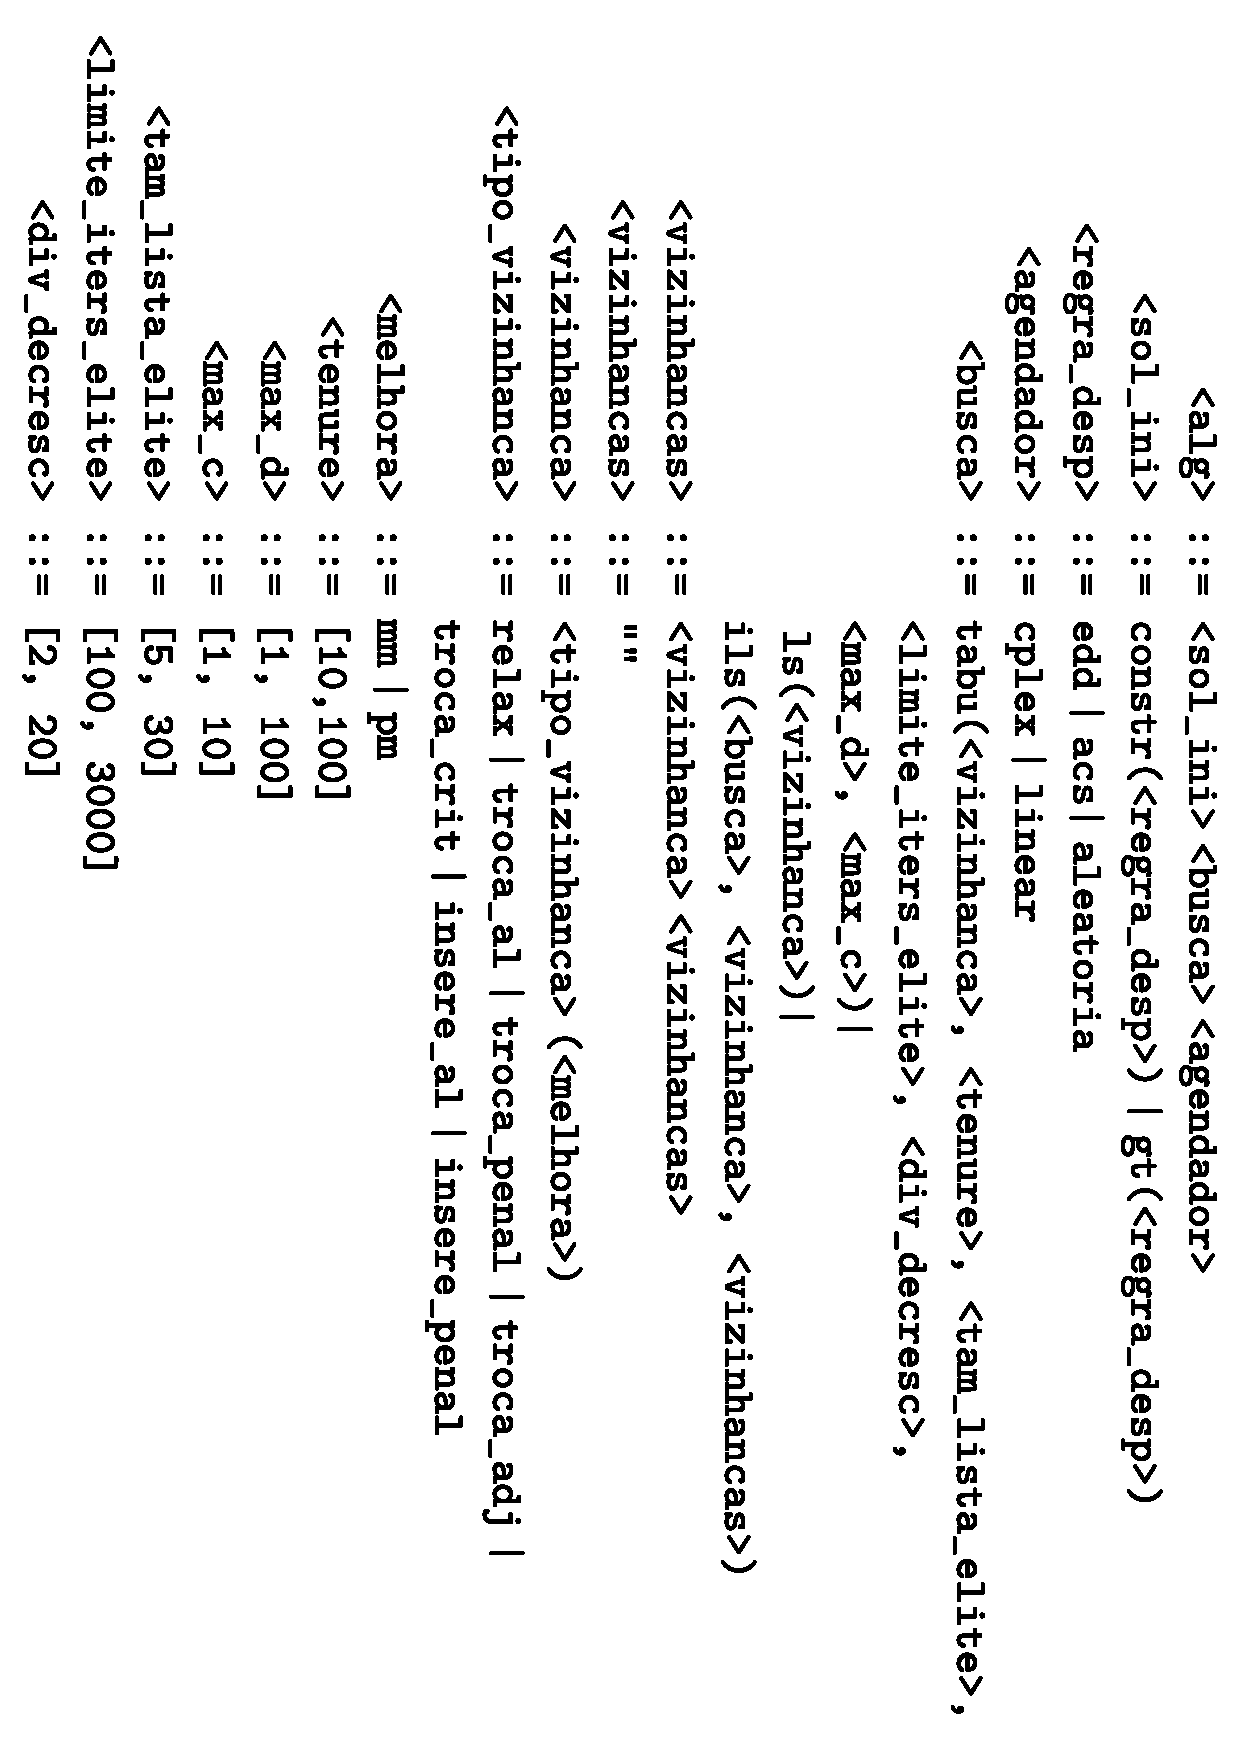
\includegraphics[angle=90, width=0.9\linewidth]{img/grammar.pdf}
    \caption*{\small \textbf{Fonte:} Os Autores.}
\end{figure}

Outro símbolo que independe das meta-heurísticas selecionadas é o agendador (\texttt{agendador}) para que o algoritmo seja capaz de avaliar a qualidade das sequências. O algoritmo é capaz de realizar este processo por meio de programação inteira (\texttt{cplex}) ou via procedimento linear que agenda as operações o mais cedo possível, mas com atraso deliberado para mitigação de penalidades de adiantamento (\texttt{linear}).

Após a derivação da solução inicial, da regra de despacho e do agendador, a gramática induz a escolha do método de busca (\texttt{busca}). Este pode ser uma \ac{LS} (\texttt{ls}), uma \ac{TS} (\texttt{tabu}) ou uma \ac{ILS} (\texttt{ils}). Os métodos de busca \texttt{ls} e \texttt{tabu} precisam apenas de uma vizinhança, que pode ser escolhida entre a \texttt{relax}, \texttt{troca\_al}, \texttt{troca\_penal}, \texttt{troca\_adj}, \texttt{troca\_crit}, \texttt{insere\_al} e \texttt{insere\_penal}. Por outro lado, a \texttt{ils} pode receber um número arbitrário de vizinhanças, e cada uma pode ser explorada por primeira melhora (\texttt{pm}) ou melhor melhora (\texttt{mm}).

A escolha do \texttt{tabu} como método de busca exige a definição de símbolos adicionais, como o tamanho da lista tabu (\texttt{tenure}). Os parâmetros da lista de elementos elite: o tamanho da lista (\texttt{tam\_list\_elite}), o número máximo de iterações para que um elemento da lista seja recuperado (\texttt{limite\_iters\_elite}) e o número que divide o limite de iterações quando nenhuma melhoria é encontrada (\texttt{div\_decresc}). Já o detector de ciclos requer o ajuste do tamanho do ciclo (\texttt{max\_d}) e do limite de repetições do mesmo ciclo para identificação de estagnação (\texttt{max\_c}).

Por fim, se escolhermos a \texttt{ils} como processo de busca, é necessário selecionar outro método de busca para ser utilizado internamente. Este caráter recursivo obriga o sistema a derivar novos símbolos idênticos aos anteriores até a obtenção de uma sequência de terminais formando um algoritmo executável.

Porém, como descrito na Seção \ref{sect:bottomup}, não podemos utilizar a gramática da Figura \ref{img:gramatica_final} em um algoritmo configurador, pois essa gramática gera infinitas palavras e o algoritmo configurador espera um espaço de projeto finito. Dessa forma, a realização da configuração automática exige uma conversão dessa gramática para um conjunto de parâmetros que force a finitude do espaço de projeto. A Tabela \ref{tab:irace_parameters} detalha o resultado da conversão. Em relação à gramática, os parâmetros representam símbolos não terminais que precisam ser derivados para os possíveis valores. Além disso, a configuração do algoritmo configurador permite utilizar condições que auxiliam na limitação e controle dos algoritmos que podem ser instanciados. Os parâmetros apenas categóricos e que já eram finitos continuam os mesmos: solução inicial, regras de despacho e agendadores.

\begin{table}[h!]
\centering
\caption{Espaço de busca de parâmetros do irace.}
\label{tab:irace_parameters}
\begin{tabularx}{\textwidth}{l >{\raggedright\arraybackslash}X X}
\hline
\textbf{Parâmetro} & \textbf{Valores} & \textbf{Condição} \\ \hline
\texttt{sol\_ini} & \texttt{gt, constr} & - \\ \hline
\texttt{regra\_desp} & \texttt{edd, acs, aleatoria} & - \\ \hline
\texttt{busca$_1$} & \texttt{ls, ils, tabu} & - \\ \hline
\texttt{busca$_2$} & \texttt{ls, tabu} & \texttt{busca$_1$} $=$ `\texttt{ils}' \\ \hline
\texttt{max\_milli\_ils\_iter} & \texttt{[1000, 30000]} & \texttt{busca$_1$} $=$ '\texttt{ils}' \\ \hline
\texttt{num\_viz} & \texttt{[1, 3]} & \texttt{busca$_1$} $=$ `\texttt{ils}' \\ \hline
\texttt{viz$_1$} & Vizinhanças LS (ver legenda) & \texttt{busca$_1$} $=$ '\texttt{ls}' \texttt{OR} '\texttt{busca$_2$} $=$ '\texttt{ls}' \\ \hline
\texttt{viz\_tabu$_1$} & Vizinhanças TABU (ver legenda) & \texttt{busca$_1$} $=$ '\texttt{tabu}' \texttt{OR} '\texttt{busca$_2$}' $=$ '\texttt{tabu}'\\ \hline
\texttt{viz\_expl$_1$} & \texttt{mm, pm} & \texttt{viz}$_1$ $\neq$ '\texttt{relax}' \\ \hline
\texttt{viz$_2$} & Vizinhanças LS (ver legenda) & \texttt{num\_viz} $\geq$ 2 \texttt{AND} \texttt{busca$_1$} $=$ '\texttt{ils}' \texttt{AND} \texttt{busca$_2$} $=$ '\texttt{ls}' \\ \hline
\texttt{viz\_tabu$_2$} & Vizinhanças TABU (ver legenda) & \texttt{num\_viz} $\geq$ 2 \texttt{AND} \texttt{busca$_1$} $=$ '\texttt{ils}' \texttt{AND} \texttt{busca$_2$} $=$ '\texttt{tabu}' \\ \hline
\texttt{viz\_expl$_2$} & \texttt{mm, pm} & \texttt{num\_viz} $\geq$ 2 \texttt{AND} \texttt{viz}$_2$ $\neq$ '\texttt{relax}'\\ \hline
\texttt{viz$_3$} & Vizinhanças LS (ver legenda) & \texttt{num\_viz} $\geq$ 3 \texttt{AND} \texttt{busca$_1$} $=$ '\texttt{ils}' \texttt{AND} \texttt{busca$_2$} $=$ '\texttt{ls}' \\ \hline
\texttt{viz\_tabu$_3$} & Vizinhanças TABU (ver legenda) & \texttt{num\_viz} $\geq$ 3 \texttt{AND} \texttt{busca$_1$} $=$ '\texttt{ils}' \texttt{AND} \texttt{busca$_2$} $=$ '\texttt{tabu}' \\ \hline
\texttt{viz\_expl$_3$} & \texttt{mm, pm} & \texttt{num\_viz} $\geq$ 3 \texttt{AND} \texttt{viz}$_3$ $\neq$ '\texttt{relax}'\\ \hline
\texttt{agendador} & \texttt{linear, cplex} & - \\ \hline
\texttt{max\_d} & \texttt{[5, 100]} & \texttt{busca$_1$} $=$ '\texttt{tabu}' \texttt{OR} '\texttt{busca$_2$} $=$ '\texttt{tabu}' \\ \hline
\texttt{max\_c} & \texttt{[1, 10]} & \texttt{busca$_1$} $=$ '\texttt{tabu}' \texttt{OR} '\texttt{busca$_2$} $=$ '\texttt{tabu}'\\ \hline
\texttt{tenure} & \texttt{[10, 100]} & \texttt{busca$_1$} $=$ '\texttt{tabu}' \texttt{OR} '\texttt{busca$_2$} $=$ '\texttt{tabu}'\\ \hline
\texttt{tam\_list\_elite} & \texttt{[5, 30]} & \texttt{busca$_1$} $=$ '\texttt{tabu}' \texttt{OR} '\texttt{busca$_2$} $=$ '\texttt{tabu}'\\ \hline
\texttt{limite\_iters\_elite} & \texttt{[100, 3000]} & \texttt{busca$_1$} $=$ '\texttt{tabu}' \texttt{OR} '\texttt{busca$_2$} $=$ '\texttt{tabu}' \\ \hline
\texttt{div\_decresc} & \texttt{[2, 20]} & \texttt{busca$_1$} $=$ '\texttt{tabu}' \texttt{OR} '\texttt{busca$_2$} $=$ '\texttt{tabu}'\\ \hline
\end{tabularx}
    \caption*{\small \textbf{Vizinhanças LS:} \texttt{troca\_adj, troca\_al, troca\_penal, troca\_crit, insere\_al, insere\_penal, relax};
\textbf{Vizinhanças TABU:} \texttt{troca\_adj, troca\_al, troca\_penal,  troca\_crit, insere\_penal, insere\_al}; \textbf{Fonte:} Os Autores.}
\end{table}

Em relação aos métodos de busca, a configuração incorpora parâmetros adicionais para a gestão da recursão limitando o nível de recursão da \ac{ILS} a 1 para evitar estruturas excessivamente complexas. Para controlar esse nível de recursão, um dos parâmetros adicionais é o segundo parâmetro de busca \texttt{busca$_2$}. Esse parâmetro só pode ser definido quando o parâmetro \texttt{busca$_1$} é igual a \texttt{ils} e não pode ser igual a \texttt{ils}. Dessa forma, uma \ac{ILS} não pode ser definida como processo de busca interno de outra \ac{ILS}.

Outro parâmetro é a quantidade de vizinhanças. Apenas a \ac{ILS} permite múltiplas vizinhanças, então esse parâmetro só fica ativo quando a primeira busca é \ac{ILS}. O intervalo desse parâmetro permite até três vizinhanças na \ac{ILS}. Junto a isso, para que o irace consiga definir as vizinhanças utilizadas e seu modo de exploração, o espaço de projeto disponibiliza três parâmetros de vizinhanças (\texttt{viz}$_x$ e \texttt{viz\_tabu}$_x$), cuja ativação depende do valor atribuído a \texttt{num\_viz}. Além disso, cada um dos parâmetros de vizinhança possui associado a ele um parâmetro que determina o tipo de exploração daquela vizinhança (\texttt{viz\_expl}$_x$) 

O último parâmetro de controle da \ac{ILS} não está tão relacionado a adaptação da gramática. O parâmetro de duração das iterações da \ac{ILS} (\texttt{max\_milli\_ils\_iter}) controla o quanto o processo de busca deve continuar explorando a vizinhança e permite ao irace equilibrar a intensificação com a diversificação da \ac{ILS}.

Apesar de todos esses parâmetros de controle da \ac{ILS}, é importante mencionar que ainda seria possível que o algoritmo configurador executasse a \ac{ILS} com duas ou três vizinhanças iguais. Não é possível limitar essa escolha apenas com a configuração representada na Tabela \ref{tab:irace_parameters}. Para melhorar o cenário de configuração, o processo emprega o mecanismo de reparação de configurações do pacote irace via \textit{script} em R, garantindo a integridade dos algoritmos gerados. O configurador submete cada configuração gerada ao \textit{script} de reparo, que identifica vizinhanças duplicadas e as substitui por componentes ainda não selecionados. 

O conjunto de parâmetros numéricos da busca tabu mantém a fidelidade à gramática original, sob a condição de ativação do modo \texttt{tabu}.

Por fim, também relacionado à \ac{TS}, cada parâmetro de vizinhança aparece duplicado. Isso acontece pois, como mencionado anteriormente, a busca tabu não suporta a vizinhança \texttt{relax} e, por isso, essa vizinhança só está disponível quando um dos dois parâmetros de busca for igual a \texttt{ls}.

\subsection{Instâncias de treino}

A obtenção de resultados precisos na configuração automática exige a separação entre os conjuntos de instâncias de treino e de teste, conforme a fundamentação da Seção \ref{sect:ref_conf_auto_configuradores}. Para isso, a metodologia estabelece a geração de novas instâncias para a composição do conjunto de treinamento. O procedimento de geração segue rigorosamente as etapas detalhadas na Seção \ref{sect:materiais}. Além disso, o processo de validação submete cada instância gerada ao solver CPLEX por um período de uma hora, sob paralelismo de 4 núcleos. O critério de seleção descarta automaticamente instâncias para as quais o solver localiza a solução ótima dentro do limite temporal estabelecido. Essa estratégia resulta em um conjunto de treinamento composto por instâncias que desafiam a capacidade de resolução de modelos de programação inteira em tempo hábil.

Como descrito na metodologia, o conjunto de testes possui 72 instâncias com diferentes combinações de tamanhos. Nesse sentido, a etapa de geração produziu 72 instâncias, respeitando a paridade de tamanhos e combinações em relação ao conjunto de teste descrito na metodologia.

\subsection{Execução do irace}

A integração do algoritmo configurável, do conjunto de treinamento e da definição do espaço de busca no pacote \textit{irace} consolida os elementos fundamentais para o início do processo de configuração. Para completar essa coleção, o processo estabelece um orçamento de configuração de 25.000 execuções para o algoritmo. Cada execução limita-se ao tempo de 60 segundos, critério baseado no desempenho médio dos algoritmos de estado da arte. Além disso, o sistema executa o \textit{irace} de forma paralela em 6 \textit{threads}. Em contrapartida, as chamadas ao solver CPLEX, tanto em vizinhanças quanto em agendamentos, operam estritamente sem paralelismo para garantir a integridade dos testes de desempenho individual.

O repositório \cite{leles2026jitjss} disponibiliza o código-fonte, \textit{scripts}, instâncias e as configurações completas utilizadas no experimento.

\section{Análise} \label{sect:analise}

A execução do pacote irace sobre o espaço de projeto detalhado anteriormente executou 10 iterações por aproximadamente 60 horas, utilizando cerca de 360 horas de processamento total, quando somados os tempos de uso de cada núcleo de processamento.

Organizaremos os resultados deste trabalho em duas subseções. Na primeira, argumentaremos a validade e a confiabilidade dos resultados do processo de calibração. Na segunda subseção, apresentaremos os testes das configurações no conjunto de instâncias de teste para comparação com as soluções do estado da arte.

\subsection{Validade do processo de configuração}

Primeiramente, a Tabela \ref{tab:irace_elites_vertical} apresenta as cinco configurações elite selecionadas pelo pacote irace como as mais eficazes para a conjunto de instâncias proposto. Nessa tabela, cada coluna representa uma das 5 melhores configurações encontradas pelo irace. Cada linha representa um parâmetro do algoritmo e os valores que cada configuração define para ele. A tabela omite os parâmetros não instanciados pelo configurador para este conjunto específico de elite.

\begin{table}[ht]
\centering
\caption{Configurações Elite Finais}
\label{tab:irace_elites_vertical}
\resizebox{\textwidth}{!}{
\begin{tabular}{lcccccc}
\hline
\textbf{Parâmetro} & \textbf{C1} & \textbf{C2} & \textbf{C3} & \textbf{C4} & \textbf{C5} \\ \hline
\texttt{sol\_ini} & \texttt{gt} & \texttt{gt} & \texttt{gt} & \texttt{gt} & \texttt{gt}  \\ 
\texttt{regra\_disp} & \texttt{edd} & \texttt{edd} & \texttt{edd} & \texttt{edd} & \texttt{edd}  \\ 
\texttt{busca$_1$} & \texttt{ils} & \texttt{ils} & \texttt{ils} & \texttt{ils} & \texttt{ils}  \\ 
\texttt{busca$_2$} & \texttt{tabu} & \texttt{tabu} & \texttt{tabu} & \texttt{tabu} & \texttt{tabu}  \\ 
\texttt{max\_milli\_ils\_iter} & \texttt{19900} & \texttt{21254} & \texttt{9713} & \texttt{5741} & \texttt{14594}\\ 
\texttt{num\_viz} & \texttt{2} & \texttt{2} & \texttt{3} & \texttt{3} & \texttt{3} \\ 
\texttt{nhood\_tabu$_1$} & \texttt{troca\_penal} & \texttt{troca\_penal} & \texttt{troca\_penal} & \texttt{troca\_al} & \texttt{troca\_penal} \\ 
\texttt{viz\_expl$_1$} & \texttt{pm} & \texttt{pm} & \texttt{pm} & \texttt{mm} & \texttt{pm}  \\ 
\texttt{nhood\_tabu$_2$} & \texttt{troca\_crit} & \texttt{troca\_crit} & \texttt{troca\_crit} & \texttt{troca\_adj} & \texttt{troca\_crit} \\ 
\texttt{viz\_expl$_2$} & \texttt{mm} & \texttt{pm} & \texttt{pm} & \texttt{pm} & \texttt{pm}  \\ 
\texttt{nhood\_tabu$_3$} & \texttt{-} & \texttt{-} & \texttt{troca\_al} & \texttt{troca\_penal} & \texttt{troca\_al} \\ 
\texttt{viz\_expl$_3$} & \texttt{-} & \texttt{-} & \texttt{pm} & \texttt{mm} & \texttt{pm}  \\ 
\texttt{agendador} & \texttt{linear} & \texttt{linear} & \texttt{linear} & \texttt{linear} & \texttt{linear}  \\ 
\texttt{max\_d} & \texttt{29} & \texttt{19} & \texttt{44} & \texttt{65} & \texttt{38}  \\ 
\texttt{max\_c} & \texttt{10} & \texttt{2} & \texttt{3} & \texttt{3} & \texttt{2}  \\ 
\texttt{tenure} & \texttt{98} & \texttt{96} & \texttt{98} & \texttt{70} & \texttt{85} \\ 
\texttt{tam\_list\_elite} & \texttt{23} & \texttt{22} & \texttt{21} & \texttt{13} & \texttt{21} \\ 
\texttt{limite\_iters\_elite} & \texttt{2788} & \texttt{2164} & \texttt{1935} & \texttt{2749} & \texttt{1353}  \\ 
\texttt{div\_decresc} & \texttt{16} & \texttt{12} & \texttt{8} & \texttt{10} & \texttt{11} \\ 
\hline
\end{tabular}
}
\caption*{\textbf{Fonte:} Os Autores.}
\end{table}

A análise das configurações revela uma uniformidade significativa nos parâmetros de alto nível, como o método de busca e o agendador. Por exemplo, os parâmetros categóricos \texttt{sol\_ini}, \texttt{regra\_disp}, \texttt{busca$_1$}, \texttt{busca$_2$} e \texttt{agendador} são iguais entre todas as configurações. De maneira similar, os parâmetros numéricos demonstram a concentração da busca em faixas de valores específicas, como ilustra o parâmetro \texttt{tenure} que reside no intervalo $[70,98]$ em todas as configurações elite.

Além disso, as escolhas referentes às vizinhanças também apresentam uma baixa diversidade estrutural. O processo de configuração descartou as vizinhanças \texttt{insere\_al}, \texttt{insere\_penal} e \texttt{relax} em favor de melhores componentes para o cenário de configuração. Ademais, todas as configurações elite utilizam as vizinhanças \texttt{troca\_penal} e quatro das cinco utilizam \texttt{troca\_crit}, indicando que a exploração do espaço de busca focada no caminho crítico e em penalidades individuais é determinante para a performance na resolução do \ac{JITJSS}.

Essa homogeneidade entre as configurações elite evidencia a convergência do modelo do \textit{irace} para uma região de alto desempenho no espaço de projeto. A redução e estabilização da variação entre as configurações elite indicaria que o modelo do irace concorda que múltiplas configurações produzem soluções de qualidade. Contudo, a avaliação visual não quantifica com precisão a variância interna desse grupo. Para essa finalidade, o estudo emprega o Coeficiente de Distância de Gower \citep{gower1971general}. Este coeficiente quantifica a dissimilaridade entre indivíduos com dados de naturezas distintas, utilizando o intervalo total do espaço de busca para a normalização das variáveis numéricas. No contexto deste trabalho, as variáveis abrangem parâmetros categóricos e numéricos.

\begin{equation} \label{eq:gower}
    d(i,j) = \frac{\sum_{k=1}^n \delta_{ij}^{(k)} s_{ij}^{(k)}}{\sum_{k=1}^n \delta_{ij}^{(k)}}
\end{equation}

O cálculo da distância de Gower ocorre de acordo com a Equação \ref{eq:gower}. Nesta fórmula, $n$ representa o número total de parâmetros do algoritmo. Além disso, $s_{ij}^{(k)}$ representa a similaridade entre as configurações $i$ e $j$ para o parâmetro $k$, sendo que:

\begin{itemize}
    \item Para variáveis categóricas: $s=0$ se $x_{ik} = x_{jk}$, e $s=1$ caso contrário;
    \item Para variáveis numéricas: $s = \frac{|x_{ik} - x_{jk}|}{R_k}$, sendo $R_k$ a amplitude do parâmetro $k$.
\end{itemize}

Por fim, a variável $\delta_{ij}^{(k)}$ assume o valor 1 quando ambos os parâmetros existem nas configurações comparadas e 0 em caso de ausência.

Contudo, a aplicação direta do coeficiente de Gower apresenta limitações na representação da semelhança funcional entre os algoritmos. Por conta das múltiplas vizinhanças, a distância de Gower superestimaria a dissimilaridade entre uma permutação diferente das mesmas três vizinhanças. Porém, devido à natureza circular do percorrimento das vizinhanças, diferentes permutações de um mesmo conjunto de vizinhanças resultam em comportamentos algorítmicos funcionalmente similares.

Para mitigar essa distorção, utilizamos o Coeficiente de Distância de Jaccard \citep{jaccard1901etude} para quantificar a semelhança entre os conjuntos de vizinhanças, desconsiderando a ordem de derivação. Ele é dado pela Equação \ref{eq:jaccard} e consiste na divisão entre o tamanho da interseção de dois conjuntos pelo tamanho da união dos dois conjuntos.

\begin{equation} \label{eq:jaccard}
    Jaccard(U,V) = 1 - \frac{|U \cap V|}{|U \cup V|}
\end{equation}

Dessa forma, para cada uma das 11 iterações do irace, calculamos a média de $d(i,j)$ para cada um dos pares formados pelas 5 configurações elite de cada iteração. O valor dessa média das distâncias entre as configurações pode ser visto no gráfico da Figura \ref{img:grafico_variancia}.

\begin{figure}[h!] 
    \centering 
    \caption{Gráfico da variância da distância de Gower entre as configurações elite pelas iterações do irace.}
    \label{img:grafico_variancia}
    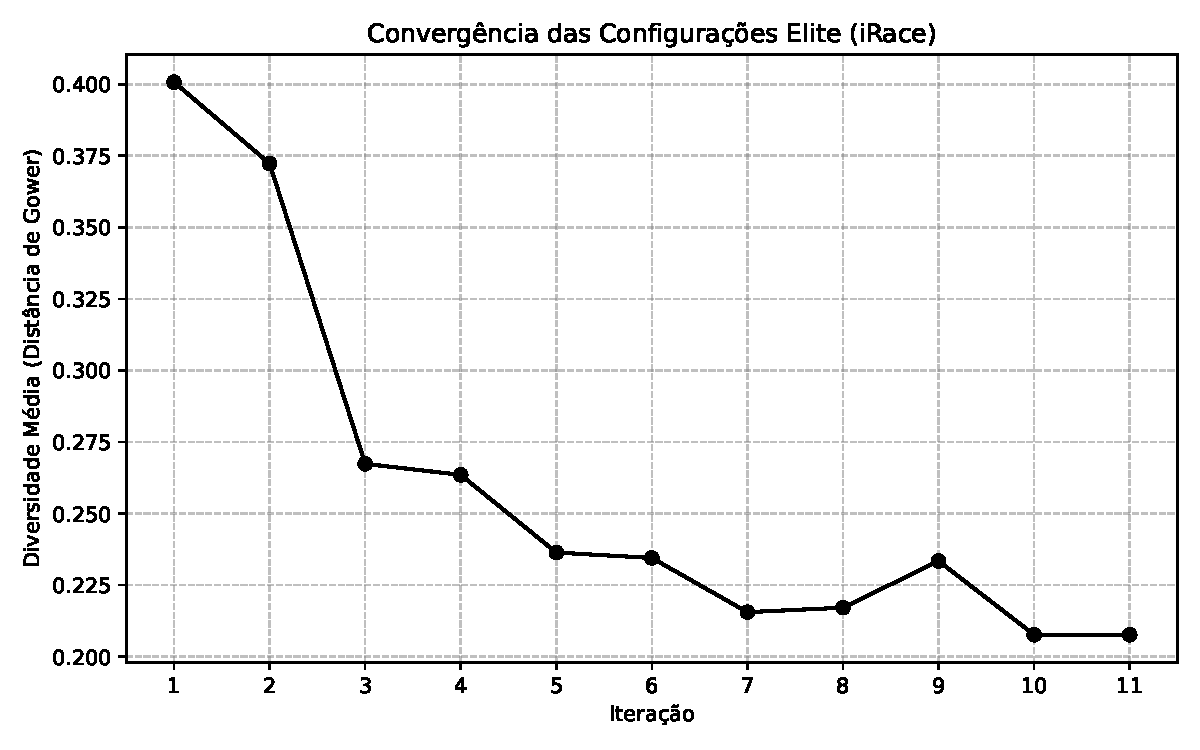
\includegraphics[width=0.9\linewidth]{img/grafico_convergencia.pdf}
    \caption*{\small \textbf{Fonte:} Os Autores.}
\end{figure}

O gráfico da Figura \ref{img:grafico_variancia} demonstra a redução progressiva da variância entre as configurações elite ao longo das iterações. Nesse sentido, a estabilização da variância na segunda metade do processo confirma a convergência do modelo de parâmetros para uma região de consenso, indicando que o processo de exploração atingiu maturidade no espaço de projeto.

Antes mesmo de realizar qualquer teste com as configurações elite, a análise das configurações elite permite a correlação direta com a literatura de \ac{JITJSS}. Por exemplo, a seleção de múltiplas vizinhanças no processo de busca. O processo de configuração pelo \textit{irace} ratifica a eficácia dessa estratégia, corroborando as abordagens de \cite{ahmadian2021meta} e \cite{wang2014variable}. Este cenário fornece um forte indício de que a exploração via vizinhança única é insuficiente diante da dificuldade do problema.

Além disso, diferentemente dos trabalhos citados, o presente trabalho propõe arquiteturas baseadas em uma Busca Tabu Iterada. Ou seja, o processo de configuração identificou que a integração de mecanismos tabu proporciona ganhos de desempenho à busca, mesmo em estruturas de múltiplas vizinhanças.

A predominância da solução inicial via \ac{GT}, associada à regra \texttt{edd}, reafirma a robustez desta combinação para o \ac{JITJSS}.

\subsection{Teste das configurações}

A convergência do processo de configuração para um grupo de algoritmos com características análogas fundamenta a etapa de testes em instâncias da literatura e a posterior comparação com o estado da arte. Para isso, a métrica de qualidade para cada instância consiste no desvio percentual em relação ao melhor valor conhecido da instância, conforme estabelecido pela Equação \ref{eq:desv_percent}. Nela, $S$ corresponde ao nosso resultado e $M$ ao melhor resultado conhecido para a instância. Ou seja, nesta escala, valores positivos indicam desempenho inferior à literatura, enquanto valores negativos apontam a superação dos marcos registrados.

\begin{equation} \label{eq:desv_percent}
     \frac{S-M}{M} * 100
\end{equation}

O procedimento inicial envolve a aplicação das configurações elite sobre o conjunto de teste. Por conta dos componentes estocásticos presentes nos algoritmos, geramos 5 \textit{seeds} aleatórias e realizamos a execução de cada configuração 5 vezes em cada instância, utilizando uma \textit{seed} diferente em cada execução.

% A distinção entre as instâncias de treinamento e de teste implica que a performance superior no primeiro conjunto não garante a liderança absoluta no segundo, fenômeno ilustrado na Tabela \ref{tab:results_confs}.
A Tabela \ref{tab:results_confs} contém um resumo do desempenho de cada configuração elite em comparação com o estado da arte. Cada coluna dessa tabela representa uma das configurações elite e as linhas contém: o número de instâncias nas quais o melhor resultado entre as cinco execuções é igual ou melhor ao estado da arte e o número de instâncias nas quais a mediana entre as cinco execuções é melhor ou igual ao estado da arte.
% Embora a configuração C1 tenha liderado o ranking no conjunto de treinamento, a C5 demonstrou maior capacidade de generalização ao atingir o maior volume de resultados iguais ou superiores ao estado da arte no conjunto de teste (34 instâncias no total).
Com isso, como representado na tabela, a configuração C1 demonstrou maior capacidade de generalização ao atingir o maior volume de resultados melhores ou iguais ao estado da arte no conjunto de teste (52 instâncias no total).

\begin{table}[ht]
\centering
\caption{Resumo dos resultados das configurações elite.}
\label{tab:results_confs}
% Substituímos tabular por tabularx e \resizebox por \textwidth
\begin{tabularx}{\textwidth}{Xcccccc}
\hline
\textbf{Parâmetro} & \textbf{C1} & \textbf{C2} & \textbf{C3} & \textbf{C4} & \textbf{C5} \\ \hline
Número de instâncias nas quais a melhor das soluções geradas pela configuração C1 é melhor ou igual ao estado da arte & 52 & 48 & 47 & 43 & 48  \\ 
Número de instâncias nas quais a mediana das soluções geradas pela configuração C1 é melhor ou igual ao estado da arte & 32 & 26 & 30 & 32 & 28  \\ 
\hline
\end{tabularx}
\caption*{\small \textbf{Fonte:} Os Autores.}
\end{table}

Dada a equivalência de desempenho entre os indivíduos elite, as análises subsequentes concentram-se na configuração C1. As tabelas \ref{tab:results_10}, \ref{tab:results_15} e \ref{tab:results_20} detalham os resultados para instâncias de 10, 15 e 20 tarefas, respectivamente, estabelecendo o comparativo com os resultados da literatura. Essas tabelas identificam as instâncias na primeira coluna e cada uma das colunas subsequentes contém os resultados dos diferentes trabalhos que compõem o estado da arte. Por fim, as duas últimas colunas representam os resultados do presente trabalho de forma que $B$ representa o melhor resultado obtido entre cinco execuções da configuração e a coluna $M$ representa a mediana dos resultados obtidos entre cinco execuções. Os resultados que representam o melhor valor encontrada para a respectiva instância são destacados em negrito nessas tabelas.

\begin{table}
\centering
\caption{Resultados da configuração C1 para as instâncias de teste de 10 tarefas.}
\label{tab:results_10}
\resizebox{\textwidth}{!}{
\begin{tabular}{lcccccccc}
\hline
\textbf{Instância}                & \textbf{Cplex}           & \textbf{[1]}          & \textbf{[2]}            & \textbf{[3]}        & \textbf{[4] }      & \textbf{[5]}        & \textbf{$B$} & \textbf{$M$}  \\
\hline
loose-equal-1-10x2  & \textbf{224,84} & \textbf{224,84} & \textbf{224,84} & \textbf{224,84} & \textbf{224,84} & \textbf{224,84}    & \textbf{224,84}       & \textbf{224,84}         \\
loose-equal-2-10x2  & \textbf{319,37} & 324,43          & \textbf{319,37} & \textbf{319,37} & \textbf{319,37} & \textbf{319,37}    & \textbf{319,37}       & \textbf{319,37}         \\
loose-equal-1-10x5  & 1738,05         & 1733,38         & 1738,05         & \textbf{1719,63} & 1725,16         & \textbf{1719,63}  & \textbf{1719,63}      & 1738,63                \\
loose-equal-2-10x5  & 971,96          & 968,89          & \textbf{967,73} & \textbf{967,73} & 968,05          & \textbf{967,73}    & \textbf{967,63}       & \textbf{967,73}                  \\
loose-equal-1-10x10 & 360,74          & 366,77          & 365,81          & 364,39          & 360,56          & \textbf{360,33}    & 360,74                & 364,59                  \\
loose-equal-2-10x10 & 251,86          & \textbf{249,85} & 252,99          & \textbf{249,85} & \textbf{249,85} & \textbf{249,85}    & \textbf{249,85}       & \textbf{249,85}         \\
loose-tard-1-10x2   & \textbf{416,44} & \textbf{416,44} & \textbf{416,44} & \textbf{416,44} & \textbf{416,44} & \textbf{416,44}    & \textbf{416,44}       & \textbf{416,44}         \\
loose-tard-2-10x2   & \textbf{137,94} & \textbf{137,94} & \textbf{137,94} & \textbf{137,94} & \textbf{137,94} & \textbf{137,94}    & \textbf{137,94}       & \textbf{137,94}         \\
loose-tard-1-10x5   & 176,83          & \textbf{175,08} & \textbf{175,08} & \textbf{175,08} & \textbf{175,08} & \textbf{175,08}    & \textbf{175,08}       & \textbf{175,08}                  \\
loose-tard-2-10x5   & 492,05          & 525,88          & 499,93          & \textbf{485,06} & 488,6           & 486,93             & \textbf{485,06}       & \textbf{485,06}         \\
loose-tard-1-10x10  & 375,71          & 383,84          & 380,26          & \textbf{374,2}  & \textbf{374,2}  & 375,58             & \textbf{374,2}        & 386,4                  \\
loose-tard-2-10x10  & \textbf{144,94} & \textbf{144,94} & 144,99          & \textbf{144,94} & \textbf{144,94} & \textbf{144,94}    & \textbf{144,94}       & \textbf{144,94}         \\
tight-equal-1-10x2  & \textbf{461,96} & \textbf{461,96} & \textbf{461,96} & \textbf{461,96} & \textbf{461,96} & \textbf{461,96}    & \textbf{461,96}       & \textbf{461,96}         \\
tight-equal-2-10x2  & \textbf{448,32} & \textbf{448,32} & \textbf{448,32} & \textbf{448,32} & \textbf{448,32} & \textbf{448,32}    & \textbf{448,32}       & \textbf{448,32}         \\
tight-equal-1-10x5  & \textbf{689,11} & \textbf{689,11} & \textbf{689,11} & \textbf{689,11} & \textbf{689,11} & \textbf{689,11}    & \textbf{689,11}       & 690,29                  \\
tight-equal-2-10x5  & \textbf{763,24} & 770,49          & 764,03          & \textbf{763,24} & \textbf{763,24} & \textbf{763,24}    & \textbf{763,24}       & \textbf{763,24}         \\
tight-equal-1-10x10 & 1281,66         & \textbf{1276,23} & 1277,44         & \textbf{1276,23} & \textbf{1276,23} & 1279,82         & 1281,66      & 1301,46                 \\
tight-equal-2-10x10 & 1885,25         & 1885,25         & 1871,23         & 1866,92         & 1865,94 & 1886,93                    & \textbf{1865,93}      & 1873,64                 \\
tight-tard-1-10x2   & \textbf{179,46} & \textbf{179,46} & \textbf{179,46} & \textbf{179,46} & \textbf{179,46} & \textbf{179,46}    & \textbf{179,46}       & \textbf{179,46}         \\
tight-tard-2-10x2   & \textbf{145,37} & \textbf{145,37} & \textbf{145,37} & \textbf{145,37} & \textbf{145,37} & \textbf{145,37}    & \textbf{145,37}       & \textbf{145,37}         \\
tight-tard-1-10x5   & \textbf{379,19} & 380,82          & 380             & \textbf{379,19} & \textbf{379,19} & \textbf{379,19}    & 386,57                & 389,43                  \\
tight-tard-2-10x5   & 635,93          & \textbf{627,45} & 628,68          & \textbf{627,45} & 628,02          & \textbf{627,45}    & \textbf{627,45}       & \textbf{627,45}         \\
tight-tard-1-10x10  & 687,65          & 717,85          & 746,03          & 668,14          & \textbf{667,97} & 669,15             & 669,93                & 687,65                  \\
tight-tard-2-10x10  & 779,17          & 780,82          & 785,79          & \textbf{777,85} & 778,32          & 780,74             & 780,66                & 804,23                  \\
\hline
\end{tabular}
}
\caption*{\small \textbf{Fonte:} A coluna Cplex foi retirada de \cite{ahmadian2021meta} e cada coluna numerada representa os resultados de um trabalho: \textbf{[1]} \cite{dos2010combination}, \textbf{[2]} \cite{wang2014variable}, \textbf{[3]} \cite{ahmadian2021meta}, \textbf{[4]} \cite{abderrazzak2022adaptive} e \textbf{[5]} \cite{sabri2023reinforcement}.}
\end{table}


\begin{table}
\centering
\caption{Resultados da configuração C1 para as instâncias de teste de 15 tarefas.}
\label{tab:results_15}
\resizebox{\textwidth}{!}{
\begin{tabular}{lcccccccc}
\hline
\textbf{Instância}                & \textbf{Cplex}           & \textbf{[1]}          & \textbf{[2]}            & \textbf{[3]}        & \textbf{[4] }      & \textbf{[5]}        & \textbf{$B$} & \textbf{$M$}   \\
\hline
loose-equal-1-15x2  & \textbf{1041,33} & \textbf{1041,33} & \textbf{1041,33} & \textbf{1041,33} & \textbf{1041,33} & \textbf{1041,33} & \textbf{1041,33}    & \textbf{1041,33}  \\
loose-equal-2-15x2  & \textbf{497,97}  & \textbf{497,97}  & 514,72          & 512,54          & \textbf{497,97}  & \textbf{497,97}    & \textbf{497,97}     & 505,16           \\
loose-equal-1-15x5  & 3457,57         & 3220,16         & 3321,54         & 3272,46         & 3258,72         & 3229,16               & \textbf{3196,85}    & 3247,89  \\
loose-equal-2-15x5  & 3437,32         & 3328,86         & 3310,27         & 3260,81         & 3255,13         & \textbf{3251,84}      & 3274,38             & 3290,70                 \\
loose-equal-1-15x10 & \textbf{875,74}  & 1008,28         & 977,43          & 906,49          & 897,51          & 913,26               & 898,99              & 938,80                \\
loose-equal-2-15x10 & 1587,09         & 1720,18         & 1584,44         & \textbf{1487,33} & 1538,27         & 1492,11              & 1554,18             & 1594,60                \\
loose-tard-1-15x2   & \textbf{654,84}  & \textbf{654,84}  & \textbf{654,84}  & \textbf{654,84}  & \textbf{654,84}  & \textbf{654,84}  & \textbf{654,84}     & \textbf{654,84}   \\
loose-tard-2-15x2   & 293,17          & \textbf{279,71}  & 297,54          & 285,16          & 289,36          & \textbf{279,71}      & \textbf{279,71}     & 290,88           \\
loose-tard-1-15x5   & 1281,87         & 1320,93         & 1315,47         & 1281    & 1292,28         & 1317,56                       & \textbf{1280,74}    & 1281,41          \\
loose-tard-2-15x5   & 335,55          & 329,47          & 335,55          & 328,26  & 330,14          & 332,25                        & \textbf{327,60}     & 328,88           \\
loose-tard-1-15x10  & \textbf{277}     & 297,19          & 296,6           & \textbf{277}     & \textbf{277}     & \textbf{277}       & 281,45              & 287,03              \\
loose-tard-2-15x10  & 597,93  & 713,97          & 664,13          & 601,24          & 627,81          & 603,67                        & \textbf{587,24}     & \textbf{592,31}         \\
tight-equal-1-15x2  & 3366,66         & \textbf{3344,54} & \textbf{3344,54} & \textbf{3344,54} & \textbf{3344,54} & \textbf{3344,54}  & \textbf{3344,54}    & \textbf{3344,54}   \\
tight-equal-2-15x2  & \textbf{1479,76} & \textbf{1479,76} & \textbf{1479,76} & \textbf{1479,76} & \textbf{1479,76} & \textbf{1479,76} & \textbf{1479,76}    & \textbf{1479,76}   \\
tight-equal-1-15x5  & 1412,71         & 1369,06         & 1345,21         & 1342,3          & 1343,08         & 1345,18               & \textbf{1318,68}    & \textbf{1318,68}   \\
tight-equal-2-15x5  & 2782,17         & 2630,06         & 2709,13         & 2641,28         & \textbf{2563,16} & 2602,99               & 2626,67             & 2651,16           \\
tight-equal-1-15x10 & 7167,59         & 7380,76         & 8120,43         & 6820,87         & 6811,54 & 7115,63                       & \textbf{6610,44}    & \textbf{6748,88}           \\
tight-equal-2-15x10 & 5407,42         & 4893,44         & 4966,34         & 4760,48         & 4801,47         & 4757,06                & \textbf{4652,41}    & \textbf{4730,08}    \\
tight-tard-1-15x2   & 806,92          & \textbf{790,5}   & 790,66          & \textbf{790,5}   & \textbf{790,5}   & \textbf{790,5}     & \textbf{790,5}      & \textbf{790,5}       \\
tight-tard-2-15x2   & \textbf{905,37}  & \textbf{905,37}  & \textbf{905,37}  & \textbf{905,37}  & \textbf{905,37}  & \textbf{905,37}   & \textbf{905,37}     & \textbf{905,37}      \\
tight-tard-1-15x5   & 1371,29         & 1371,37         & 1426,97         & 1359,18         & 1366,45         & \textbf{1341,69}       & 1358,21             & 1359,18            \\
tight-tard-2-15x5   & 721,46          & 691,1           & 725,72          & 681,27          & 677,8           & 695,08                 & \textbf{677,57}     & 681,62     \\
tight-tard-1-15x10  & 815,03          & 800,87          & 832,08          & 767,26  & 770,91          & 775,4                          & \textbf{757,83}     & 785,75        \\
tight-tard-2-15x10  & 1267,53         & 1310,04         & 1452,9          & 1224,82         & 1243,52         & 1226,23                & \textbf{1170,94}    & \textbf{1172,30}     \\
\hline
\end{tabular}
}
\caption*{\small \textbf{Fonte:} A coluna Cplex foi retirada de \cite{ahmadian2021meta} e cada coluna numerada representa os resultados de um trabalho: \textbf{[1]} \cite{dos2010combination}, \textbf{[2]} \cite{wang2014variable}, \textbf{[3]} \cite{ahmadian2021meta}, \textbf{[4]} \cite{abderrazzak2022adaptive} e \textbf{[5]} \cite{sabri2023reinforcement}.}
\end{table}

\begin{table}
\centering
\caption{Resultados da configuração C1 para as instâncias de teste de 20 tarefas.}
\label{tab:results_20}
\resizebox{\textwidth}{!}{
\begin{tabular}{lcccccccc}
\hline
\textbf{Instância}                & \textbf{Cplex}           & \textbf{[1]}          & \textbf{[2]}            & \textbf{[3]}        & \textbf{$B$} & \textbf{$M$}   \\
\hline
loose-equal-1-20x2  & 2565,51 & \textbf{2548,95} & 2551,22 & \textbf{2548,95}                   & \textbf{2548,95}     & 2549,19               \\
loose-equal-2-20x2  & 3105,34 & \textbf{3069,13} & 3070,16 & \textbf{3069,13} & \textbf{3069,13}     & \textbf{3069,13}               \\
loose-equal-1-20x5  & 8271,34 & 7545,44 & 7758,02 & 7524,13                   & \textbf{7487,77}     & 7666,29              \\
loose-equal-2-20x5  & 7793,45 & 7252,81 & 7302,01 & 7059,38                   & \textbf{7022,53}     & 7128,87               \\
loose-equal-1-20x10 & 5597,4  & 5260,48 & 5476,47 & 4651,31                   & \textbf{4592,02}     & 4687,60               \\
loose-equal-2-20x10 & 1862,41 & 1987,65 & 1718,08 & \textbf{1597,89}          & 1608,61              & 1701,42                        \\
loose-tard-1-20x2   & 1265,36 & 1206,97 & 1205,59 & 1206,4                     & \textbf{1203,88}     & 1206,97               \\
loose-tard-2-20x2   & 772,89  & \textbf{769,35}  & 790,12 & \textbf{769,35}   & 771,06               & 776,01                          \\
loose-tard-1-20x5   & 3548,14 & 2938,24 & 3517,2  & \textbf{2931,11}          & 2936,63              & 3068,78                         \\
loose-tard-2-20x5   & 4048,77 & 3722,61 & 3684,67 & 3627,51                   & \textbf{3617,49}     & 3646,58               \\
loose-tard-1-20x10  & 6494,34 & 5093,89 & 5478,21 & 4817,32                   & \textbf{4789,13}     & 5114,72               \\
loose-tard-2-20x10  & 1545,95 & 1570,64 & 1599,55 & \textbf{1401,28}          & 1516,95              & 1531,54                         \\
tight-equal-1-20x2  & 1940,06 & 1937,49 & 1939,11 & 1936,45                   & \textbf{1933,72}     & \textbf{1933,72}               \\
tight-equal-2-20x2  & 961,44  & \textbf{941,69}  & 959,65  & 943,7            & 944,93               & 948,01                          \\
tight-equal-1-20x5  & 3013,79 & 2866,94 & 2935,95 & 2865,95                   & \textbf{2821,02}     & \textbf{2865,45}               \\
tight-equal-2-20x5  & 7233,35 & 6741,16 & 6964,91 & 6613,62                   & \textbf{6581,72}     & 6626,55               \\
tight-equal-1-20x10 & 11561,7 & 10607,2 & 11073,1 & \textbf{10378,8}          & 10534,50             & 10831,90                          \\
tight-equal-2-20x10 & 8501,42 & 7310,32 & 7317,74 & \textbf{6839,3}           & 6892,16              & 7047,16                          \\
tight-tard-1-20x2   & 1675,37 & \textbf{1671,87} & 1682,94 & 1674,6           & \textbf{1671,87}     & 1672,03               \\
tight-tard-2-20x2   & 1489,65 & \textbf{1448,66} & 1459,57 & 1451,61          & \textbf{1448,66}     & \textbf{1448,66}               \\
tight-tard-1-20x5   & 3821,29 & 3672,18 & 3669,09 & 3620,61                   & \textbf{3598,12}     & \textbf{3618,13}               \\
tight-tard-2-20x5   & 1881,02 & 1858,19 & 1976,11 & \textbf{1792,78}          & 1802,78              & 1808,36                         \\
tight-tard-1-20x10  & 4984,31 & 4853,81 & 5536,64 & 4445,59                   & \textbf{4406,01}     & \textbf{4434,02}               \\
tight-tard-2-20x10  & 4057,01 & 3358,61 & 3245,9  & \textbf{3085,54}          & 3207,33              & 3242,14                         \\
\hline
\end{tabular}
}
\caption*{\small \textbf{Fonte:} A coluna Cplex foi retirada de \cite{ahmadian2021meta} e cada coluna numerada representa os resultados de um trabalho: \textbf{[1]} \cite{dos2010combination}, \textbf{[2]} \cite{wang2014variable} e \textbf{[3]} \cite{ahmadian2021meta}.}
\end{table}

A análise dos dados revela que o algoritmo configurado igualou ou superou o estado da arte em aproximadamente 72,2\% das 72 instâncias de teste. Essa eficácia concentra-se predominantemente nas instâncias de 10 tarefas, nas quais o algoritmo atingiu o marco de 83\% de sucesso em relação aos melhores valores da literatura. Além disso, a análise das medianas corrobora a robustez da configuração C1, a qual igualou ou superou os marcos bibliográficos em 44,4\% das instâncias.
% a configuração C5 obteve melhorias incrementais em casos específicos. Nesse sentido, a hipótese central reside na proximidade desses resultados em relação ao limite inferior de otimalidade, especialmente nos cenários de menor escala, o que restringe o potencial de ganho de novas heurísticas..

Os dados expostos indicam uma redução gradual na eficácia da mediana conforme a escala das instâncias aumenta. Contudo, o desvio médio das medianas em relação às melhores soluções individuais é de apenas 1,06\%, evidenciando a estabilidade do método estocástico frente a variações de sementes aleatórias.

Embora os marcos de desempenho demonstrem competitividade, a análise prévia baseia-se no melhor valor conhecido para cada instância. Esta métrica representa um limite superior composto pelos melhores resultados de todos os trabalhos da literatura combinados. Dessa forma, a comparação individual apresentada na Tabela \ref{tab:comparacao_estado} isola o desempenho da proposta frente a cada método do estado da arte de maneira independente. As colunas organizam os resultados por autor, enquanto as linhas quantificam o número de instâncias nas quais a configuração C1 obteve desempenho igual ou superior ao de cada método de referência. Com isso, os resultados evidenciam que a configuração gerada por este estudo apresenta qualidade superior em comparações diretas com cada trabalho da literatura.

\begin{table}[ht]
\centering
\caption{Comparação individual entre este trabalho e algoritmos da literatura.}
\label{tab:comparacao_estado}
\begin{tabularx}{\textwidth}{Xcccccc}
\hline
\textbf{}                 & \textbf{[1]}          & \textbf{[2]}            & \textbf{[3]}        & \textbf{[4] }      & \textbf{[5]}   \\ \hline
Porcentagem das instâncias nas quais a melhor das soluções geradas pela configuração C1 é melhor ou igual aos resultados de um trabalho & 94,44 & 97,22 & 77,77 & 79,16 & 81,25  \\ 
Porcentagem das instâncias nas quais a mediana das soluções geradas pela configuração C1 é melhor ou igual aos resultados de um trabalho & 75 & 88,88 & 50 & 62,5 & 62,5  \\ 
\hline
\end{tabularx}
\caption*{\small \textbf{Fonte:} cada coluna numerada representa os resultados de um trabalho: \textbf{[1]} \cite{dos2010combination}, \textbf{[2]} \cite{wang2014variable}, \textbf{[3]} \cite{ahmadian2021meta}, \textbf{[4]} \cite{abderrazzak2022adaptive} e \textbf{[5]} \cite{sabri2023reinforcement}.}
\end{table}

Como mencionado anteriormente, todas as execuções do algoritmo levam 60 segundos. O algoritmo de \ac{ILS} opera sem mecanismos de detecção de convergência das soluções, gastando o tempo limite de 60 segundos em todas as execuções. Entretanto, a localização da solução final ocorre, em média, aos 21,1 segundos de execução. Em instâncias de 10 tarefas, este marco reduz-se para 9 segundos. Esses indicadores sugerem que a integração de critérios de convergência otimizará a eficiência computacional do algoritmo, permitindo a obtenção de resultados da mesma qualidade em frações do tempo total estabelecido.


\chapter{Conclusão} \label{chapt:conclusao}

Neste trabalho, apresentamos a aplicação das técnicas de \ac{AAC} e \ac{AAD} para a resolução do problema \ac{JITJSS}. A motivação central fundamentou-se na eliminação do viés humano e do esforço mecânico associados ao desenvolvimento manual de heurísticas, propondo, em contrapartida, um espaço de projeto estruturado e explorado de forma sistemática pelo pacote \textit{irace}.

Nossas contribuições incluem a nova vizinhança \texttt{troca\_crit} para o problema \ac{JITJSS}, construída a partir do estudo das componentes da literatura. Com isso, a partir da aplicação das técnicas de \ac{AAD}, constatamos que a inclusão no espaço de projeto dessa vizinhança, focada no caminho crítico individual de operações atrasadas, mostrou-se determinante, sendo integrada pelo configurador em 80\% das soluções de elite.

Além disso, como resultado do processo de \ac{AAD}, propomos um novo algoritmo estado da arte para o \ac{JITJSS}. O algoritmo proposto superou ou igualou o estado da arte da literatura em 72,2\% das 72 instâncias de teste. Adicionalmente, ao analisarmos a eficiência temporal, observamos que, embora o limite de tempo estivesse fixado em 60 segundos, o algoritmo encontrou a solução final, em média, aos 21,1 segundos de execução, evidenciando uma rápida velocidade de convergência.

Dessa forma, concluímos que os experimentos conduzidos validaram a hipótese inicial de que o projeto automático é capaz de derivar algoritmos competitivos. Outrossim, os experimentos demonstraram que as componentes algoritmicas propostas são particularmente efetivas gerando algoritmos que superam o estado da arte na maioria das instâncias. Nessa perspectiva, o processo de configuração utilizando o \textit{irace} convergiu para uma região de alto desempenho, resultando na configuração elite C1, caracterizada como uma Busca Tabu Iterada. 

Como limitações da abordagem atual, apontamos a ausência de um critério de parada antecipada na heurística de busca e a restrição do nível de recursão da gramática para evitar a complexidade excessiva no processo de amostragem do configurador.

Para trabalhos futuros, listamos as seguintes frentes de pesquisa:
\begin{itemize}
    \item \textbf{Ampliação do Espaço de Projeto:} Inclusão de novos operadores de busca de solução única, como Algoritmos Genéticos, Busca em Grandes Vizinhanças ou Recozimento Simulado, diretamente como blocos terminais da gramática;
    \item \textbf{Análise de Instâncias de Larga Escala:} Aplicação do algoritmo gerado sobre novos conjuntos de instâncias com dimensões superiores a 20 tarefas e 10 máquinas para avaliar o comportamento do algoritmo sob estresse computacional.
    \item \textbf{Aplicação sobre novos domínios:} Aplicação do algoritmo gerado em novos problemas com propriedades similares ao \ac{JITJSS}. A exemplo, temos o problema \textit{Just-In-Time Job Shop with Setup Times} que é idêntico ao \ac{JITJSS}, mas adicionando tempos de troca entre operações processadas na mesma máquina.
\end{itemize}

% Aqui vem a parte da bibliografia: use o comando \ppgccbibliography indicando
% apenas o nome do arquivo .bib (sem a extensão).
\ppgccbibliography{bibfile}


% Este comando encapsula o conjunto de apêndices. A sua função é fazer com que
% a numeração dos apêndices seja feita com letras maiúsculas (A, B, C, etc.) e
% a palavra "Apêndice" anteceda as entradas no Sumário.
% \begin{appendices}
% \input{ApendiceA}
% \input{ApendiceB}
% \end{appendices} % Fim dos apêndices (usar apenas depois do último apêndice)


% % Este comando encapsula o conjunto de anexos. A sua função é fazer com que a
% % numeração dos anexos seja feita com letras maiúsculas (A, B, C, etc.) e a
% % palavra "Anexo" anteceda as entradas no Sumário.
% \begin{attachments}
% % Para cada anexo, um \chapter
\chapter{Um anexo}

\dummytxta
\dummytxtb
\dummytxtc
\dummytxta
\dummytxtb
% \chapter{Outro anexo}

\dummytxta
\dummytxtb
\dummytxtc
\dummytxta
\dummytxtb
% \end{attachments} % Fim dos anexos (usar apenas depois do último anexo)


\end{document}
